%% Twoside is needed for openright, which puts chapters beginning on odd pages.
\documentclass[a4paper, 11pt, twoside, openright]{report}
\usepackage[utf8]{inputenc}
\usepackage[english]{babel}

%% Font encoding (how chars are represented in output file).
%% http://tex.stackexchange.com/questions/664/
%% http://tex.stackexchange.com/questions/44694/
\usepackage[T1]{fontenc}

%% Some T1 fonts to use ("ae" package is an alternative).
\usepackage{lmodern}

%% Better monospace font, needs to appear after lmodern.
%% incosolata is also nice but does not have single quotes or backtick
%%  chars to work with the upquote package.
\usepackage[scaled=0.82]{beramono}

%% In verbatim environments, prints the console single quote and backtick
%% characters.
\usepackage{upquote}

\usepackage{amsmath,amsthm,amssymb}
\usepackage{amsfonts}
\usepackage{fancyhdr}
\usepackage{graphicx}
\usepackage{lscape}
\usepackage{color}

%% Like verbatim, but with commands.
\usepackage{alltt}

%% \FloatBarrier
\usepackage{placeins}

%% Appendices as chapters in the {appendices} environment.
\usepackage[toc,page]{appendix}

%% Necessary to be able to put newlines in short captions.
%% Add option [justification=centering] to center multiline captions,
%% or use the string inside \captionsetup{} for individual figures.
\usepackage{caption}

%% Prevent some (not all) huge spaces around some section titles.
\usepackage[raggedright,compact]{titlesec}

%% Horizontal line below captions.
\DeclareCaptionFormat{myformat}{#1#2#3\hrulefill}
\captionsetup[figure]{format=myformat}
\captionsetup[table]{format=myformat}

%% For nice abstracts (on one page)
\usepackage{abstract}
\renewcommand{\abstractnamefont}{\normalfont\Large\bfseries}
\renewcommand{\abstracttextfont}{\normalfont}

%% Align left rather than justify text.
% \raggedright

%% A few colors.
\definecolor{blue}{rgb}{0,0,1}
\definecolor{black}{rgb}{0,0,0}
\definecolor{flashyBlue}{rgb}{0,0.5,1}
\definecolor{brownishRed}{rgb}{0.6,0.1,0.1}

%% Environement to display source code listings.
\usepackage{listings}

%% Listings defaults. To change them for a single listing, use
%% \begin{lstlisting}[<args>] where args are like the arguments to \lstset.
\lstset{
  aboveskip=0.5cm,
  % small text, monospace font
  basicstyle=\ttfamily,
  % syntax highlighting
  identifierstyle=\color{black},
  keywordstyle=\color{blue},
  stringstyle=\color{brownishRed},
  commentstyle=\color{flashyBlue}
}

\lstdefinelanguage[]{caxap}[]{Java}{
  deletestring=[b]{'}
}

%% To get line numbers every 5 lines, starting at line 1 (then 5, then 10, ...).
\newcommand{\commentsfive}{\lstset{numbers = left, stepnumber = 5, firstnumber =
    1, numberfirstline = true}}

%% Also source code highlights. Better than listings? Need to investigate.
% \usepackage{minted}

%% No left space at start of paragraph + set inter-paragraph space.
\usepackage{parskip}
\setlength{\parskip}{0.5cm}

%% Allows to use literal underscore in text and other places. The strings
%% argument allows underscore to be used in certain command that work with file
%% names, such as \input{}.
\usepackage[strings]{underscore}

%% To use links, both internal and external. Make all links blue (normally red),
%% including the links to the bibliography, which are normally green.
\usepackage[colorlinks, allcolors=blue]{hyperref}

%% A kind of box that allow verbatim text inside.
\usepackage{framed}
\setlength{\OuterFrameSep}{3mm}

\usepackage{enumitem}
	\setitemize{itemsep=-1mm}
	\setenumerate{itemsep=0mm,partopsep=0mm}
\usepackage{microtype}

\pagestyle{fancy}
\renewcommand{\sectionmark}[1]{\markright{#1}}
\renewcommand{\footrulewidth}{0.4pt}
\fancyhf{}

%% Sets the distance between a figure included in the text using the "h" option,
%% and the text. The "plus" and "minus" parts allow Latex to expand/shrink the
%% space.
\setlength{\intextsep}{20.0pt plus 2.0pt minus 2.0pt}

%% Chapter name in left page header, section name in right.
\fancyhead[LE]{\leftmark}
\fancyhead[RO]{\rightmark}

%% Footer page numbering.
\fancyfoot[LE]{\thepage}
\fancyfoot[RO]{\thepage}
\pagenumbering{arabic}

%% Makes the lines separating header & footer light grey instead of black.
\renewcommand{\headrulewidth}{0.1pt}
\renewcommand{\footrulewidth}{0.1pt}

\addtolength{\textwidth}{3cm}       % text width
\addtolength{\headwidth}{3cm}       % width of heading on each page
\addtolength{\textheight}{4cm}      % self explaining (spread by voffset)
\addtolength{\voffset}{-2cm}        % distance between top and text

\uchyph=0 % forbids splitting words that start with a capital letter
\linespread{1.1}                    % interline 1.1

\addtolength{\hoffset}{-0.6cm}      % left margin
%% Lefthand margin on even/odd numbered pages.
\setlength{\evensidemargin}{\oddsidemargin}


\DeclareGraphicsExtensions{.png,.jpg,.bmp,.msp,.pdf,.fig}

\title{
  \begin{center}
    \begin{tabular}{lp{2cm}r}
      
\includegraphics[height=4cm]{logo_ucl.png} & &
      
\includegraphics[height=4cm]{logo_epl.png}\\
    \end{tabular} \\
    \vspace{\fill}
    Université Catholique de Louvain \\
    Ecole Polytechnique de Louvain \\
    INGI Department \\
    \vspace{\fill}
    \textbf{A PEG-Based Macro System for Java}
    \vspace{\fill}
    \normalsize \\
    A thesis submitted to the Université Catholique de Louvain in accordance
    with the requirements of the degree of Master in Computer Science (120
    credits).
    \vspace{\fill}
  \end{center}
}

\date{Louvain-la-Neuve, academic year 2012 - 2013}
 \author{
   \begin{tabular}{rl}
     Author         & Nicolas \textsc{Laurent}      \\
     Supervisor     & Pr. Peter \textsc{Van Roy}    \\
     Readers        & Pr. Kim \textsc{Mens}         \\
     and            & Yves \textsc{Jaradin}
   \end{tabular}
  }

\begin{document}
\maketitle
\cleardoublepage

%%%%%%%%%%%%%%%%%%%%%%%%%%%%%%%%%%%%%%%%%%%%%%%%%%%%%%%%%%%%%%%%%%%%%%%%%%%%%%%%
\label{abstract}

\begin{abstract}

  Programming is abstracting. As such, programming languages supply us with
  abstraction facilities such as functions and classes. One such facility is the
  macro. A macro defines new language constructs, to be translated at
  compile-time into existing constructs. Macros permit the abstraction of
  patterns that cannot be abstracted by the usual abstraction facilities.

  We introduce caxap, a framework that adds a Lisp-like macro system on top of
  Java, a programming language with a complex grammar and lacking the property
  of homoiconicity. Our aim is to be as general as possible, allowing arbitrary
  syntax to be added to the language, and arbitrary computation to be done to
  translate the new syntax to the old. To that end, we use parsing expression
  grammars (PEGs) as tools to reason about and manipulate syntax.

\end{abstract}

%%%%%%%%%%%%%%%%%%%%%%%%%%%%%%%%%%%%%%%%%%%%%%%%%%%%%%%%%%%%%%%%%%%%%%%%%%%%%%%%

\cleardoublepage
\renewcommand{\abstractname}{Acknowledgements}
\begin{abstract}
  I would first like to thank my friends, which have helped me keep my sanity
  and my motivation during all these months. I'm thinking of Arnaud Beelen,
  Adrien Bibal, Etienne Martel, Anthony Popolo Cagnisi, Renaud Proye, Valentin
  Vansteenberghe and Romain Van Vooren. My thanks extend to my family, which has
  always supported me.

  I would like to thank my promoter, Peter Van Roy, for the freedom with which
  he has entrusted me. I hope I used it well. Likewise, I am grateful to Kim
  Mens and Yves Jaradin for accepting the task of being my readers. I also
  extend my thanks towards Darius Blasband for his judicious remarks. Finally,
  I'm grateful to all the professors and teaching assistants which imparted
  their knowledge to me during these five years.
\end{abstract}

%%%%%%%%%%%%%%%%%%%%%%%%%%%%%%%%%%%%%%%%%%%%%%%%%%%%%%%%%%%%%%%%%%%%%%%%%%%%%%%%

\cleardoublepage
\thispagestyle{empty}
\null\vfill

\newlength\longest
\setlength{\longest}{15cm}
\centering
\parbox{\longest}{\Large \raggedright{It is impossible to dissociate language
    from science or science from language, because every natural science always
    involves three things: the sequence of phenomena on which the science is
    based, the abstract concepts which call these phenomena to mind, and the
    words in which the concepts are expressed. To call forth a concept, a word
    is needed; to portray a phenomenon, a concept is needed.  All three mirror
    one and the same reality.}

  \raggedleft{—Antoine Lavoisier, 1789}
}

\vfill\vfill
\cleardoublepage
\raggedright

%%%%%%%%%%%%%%%%%%%%%%%%%%%%%%%%%%%%%%%%%%%%%%%%%%%%%%%%%%%%%%%%%%%%%%%%%%%%%%%%

\setcounter{tocdepth}{2}
\tableofcontents

\chapter{Macros}
\label{intro_macros}

In this chapter, we introduce the notion of \emph{macro} in all generality. We
highlight a few characteristics of macros and explain how they usually work.

%%%%%%%%%%%%%%%%%%%%%%%%%%%%%%%%%%%%%%%%%%%%%%%%%%%%%%%%%%%%%%%%%%%%%%%%%%%%%%%%
\section{Generalities}

Generally speaking, a macro is a way to convert a sequence of items into another
sequence, meant to replace the original sequence. The input and output sequences
of a macro contain the same kind of items. The macro system must define exactly
how a sequence will be converted to its replacement.

An example of macro mechanism is an application that intercepts sequences of
keystrokes and replaces them with another sequence of keystrokes, according to
rules defined by the user.

In the context of programming languages, input and output sequences contain
characters or lexical tokens.

Let us examine how programming language macros - henceforth simply \emph{macros}
- work. Three mechanisms are needed to define a macro. First, a mechanism to
define the set of input sequences matched by the macro. Second, a mechanism to
map the matched sequence to a replacement sequence. Third, a mechanism to
specify the context in which the macro can be applied: the \emph{macro
  application context}.

To support our analysis of those mechanisms, we look at caxap, and at the macro
systems from the languages C and Lisp.

%%%%%%%%%%%%%%%%%%%%%%%%%%%%%%%%%%%%%%%%%%%%%%%%%%%%%%%%%%%%%%%%%%%%%%%%%%%%%%%%
\section{Examples}

Figure \ref{macro_example} shows the definition and usage of the \texttt{unless}
construct as a macro in Java, C and Common Lisp.

\texttt{unless} is an inverted \texttt{if} construct: it executes a statement
only if a condition evaluates to \texttt{false}.

In all three languages, a macro definition ensures all three mechanisms
mentioned above are fully defined. In some cases, a mechanism may be implicit,
for instance if it is independent of any individual macro definition. The
mechanisms were: the definition of matched input sequences, the mapping from
input to output, and the specification of the macro application context.

\begin{figure}[here]
\small
\begin{lstlisting}[frame=single,language=caxap]
// caxap
macro Unless as Statement : "unless" cond:expression :body
{
  return `statement[if (!(#cond)) #body]`;
}

unless myPredicate() { myMethod(); }
// --> if (!(myPredicate()) { myMethod(); }
\end{lstlisting}

\begin{lstlisting}[frame=single,language=C]
// C
#define UNLESS(CONDITION, STATEMENT) if (!(CONDITION)) STATEMENT

UNLESS(myPredicate(), { myFunction(); })
// --> if (!(myPredicate()) { myFunction(); }
\end{lstlisting}

\begin{lstlisting}[frame=single,language=Lisp]
; Lisp
(defmacro unless (condition statement)
  `(if (not ,condition) ,statement))

(unless (myPredicate) (myFunction))
; --> (if (not (myPredicate)) (myFunction))
\end{lstlisting}
\caption{Definition and usage of the \texttt{unless} construct as a macro in
  caxap, C and Common Lisp.}
\label{macro_example}
\end{figure}

%%%%%%%%%%%%%%%%%%%%%%%%%%%%%%%%%%%%%%%%%%%%%%%%%%%%%%%%%%%%%%%%%%%%%%%%%%%%%%%%
\section{Matching Input and Defining Context}

%%%%%%%%%%%%%%%%%%%%%%%%%%%%%%%%%%%%%%%%%%%%%%%%%%%%%%%%%%%%%%%%%%%%%%%%%%%%%%%%
\subsubsection{Using Formal Grammars}

A way to describe input sequences is to use formal grammars. A formal grammar
describes a set of productions - such as the admissible input sequences - by
using rules. Each rule defines a set of production by defining how primitive
elements are composed to make up the productions. Rules may reference the set of
productions generated by other rules.

In chapter \ref{peg_intro} we describe Parsing Expression Grammars (PEG), a
particular way to define formal grammars. caxap uses PEGs to specify admissible
input sequences. Figure \ref{matching_input_example} includes a small PEG
grammar.

We can also use grammars to define the macro application context. We simply
equate the application context to an existing grammar rule. Since we introduce a
new grammar rule to describe the admissible input sequences, we position this
new rule as an alternative to the existing rule. The new rule will only be
applicable in places where the existing rule is also applicable.

Figure \ref{matching_input_example} shows how we can define \texttt{unless} in a
small imaginary language.

\begin{figure}[here]
\small
\begin{lstlisting}[frame=single]
Identifier ::= [a-z]+
Literal    ::= "true" | "false" | [0-9]+
Operator   ::= ">" | "<" | "+" | "-" | "*" | "/"
Expression ::= Identifier | Literal | Literal Operator Expression
Statement  ::= Identifier "=" Expression | "if" Expression "{" Statement* "}"
File       ::= "module" "{" Statement* "}"

macro Unless as Statement : "unless" Expression "{" Statement* "}"
\end{lstlisting}
\caption{An example containing a PEG and a macro declaration. The PEG shows how
  to match input sequences using grammar rules. The macro declaration shows how
  to define the macro application context using an existing grammar rule name.}
\label{matching_input_example}
\end{figure}

Look at the \texttt{File} rule, which is the root of the grammar. From the
content of the rule, we can see that \texttt{Unless} couldn't be matched at the
beginning of a file. It can only be matched where \texttt{Statement} can, for
instance after the input sequence \texttt{"module \{"} has been encountered. The
state \emph{after matching \texttt{"module \{"}} is a context where the
\texttt{Unless} macro could possibly be applied.

caxap uses grammar rules to define input sequences and application context.

%%%%%%%%%%%%%%%%%%%%%%%%%%%%%%%%%%%%%%%%%%%%%%%%%%%%%%%%%%%%%%%%%%%%%%%%%%%%%%%%
\subsubsection{Alternative Approaches}

Most macro-enabled languages do not allow macros to match arbitrary syntax. For
instance, Lisp and C impose that macro calls look like function calls. This
means that each macro possesses a unique name, and a number of formal
parameters. Defining a macro's input sequence then comes down to defining its
name and the expected parameters.

In Lisp and C, a macro's application context is implicit. C has actually no
application context: a macro can appear anywhere in a file. In Lisp, a macro can
appear anywhere a function could; which is almost everywhere, as long as
parentheses remain properly balanced.

%%%%%%%%%%%%%%%%%%%%%%%%%%%%%%%%%%%%%%%%%%%%%%%%%%%%%%%%%%%%%%%%%%%%%%%%%%%%%%%%
\subsubsection{Syntactic and Lexical Macros}

Macros working at the level of the syntax tree are said to be \emph{syntactic},
whereas macros working with characters or lexical tokens are said to be
\emph{lexical}.

A syntax tree is the result of a successful input parse according to a
grammar. It maps parts of the input to the grammar rules they match.

caxap and Lisp macros are syntactic. C macros are lexical. Lexical macros can
often be recognized by the fact that they do not specify macro application
contexts.

%%%%%%%%%%%%%%%%%%%%%%%%%%%%%%%%%%%%%%%%%%%%%%%%%%%%%%%%%%%%%%%%%%%%%%%%%%%%%%%%
\section{Mapping an Input Sequence to its Replacement}

There are two popular mechanisms used to map an input sequence to its
replacement.

The most general mechanism is to allow any arbitrary computation to determine
the replacement. This is what caxap does, by allowing arbitrary Java code to run
at compile-time. Lisp also works this way. Macros that allow arbitrary code to
run are called \emph{procedural macros}.

The other mechanism is to form the output sequence by injecting macro parameters
into a fixed sequence of characters or tokens. We call macros defined this way
\emph{transformative macros}. C macros are transformative: the output sequence
is created by replacing all macro parameters appearing in the macro definition
by the values supplied in the macro call. In figure \ref{macro_example}, this
means that \texttt{myPredicate()} will be substituted for \texttt{CONDITION}.

Transformative macros, however restricted, are simple. Procedural macro systems
usually provide a facility to inject input parameters into a sequence of
characters. This facility is traditionally called \emph{quasiquotation}. Figure
\ref{macro_example} features uses of quasiquotation in caxap and Lisp. We
describe caxap's quasiquotations in section \ref{quotation_manual}.

\chapter{Motivation}
\label{motivation_chapter}

Now that we have seen what macros were, I can offer some motivation for the work
presented in this thesis. In this chapter, I explain why I built a macro system
on top of Java, and describe what makes this undertaking worthwhile.

%%%%%%%%%%%%%%%%%%%%%%%%%%%%%%%%%%%%%%%%%%%%%%%%%%%%%%%%%%%%%%%%%%%%%%%%%%%%%%%%
\section{Macros in the Wild}

Macros have existed for a long time. The first trace of macros I could find is a
paper dating back to 1960. \cite{macro_assem} In that paper, professor Douglas
McIlroy proposes a macro system for an imaginary assembly language. More famous
is the 1963 paper by Timothy Hart \cite{macrodef} that introduces macros for the
Lisp language.

Macros have a long history, but tied to languages deemed old and/or obscure by
most current-day programmers. The history of macros is inextricably linked to
the history of the Lisp family of languages. Nowadays, Lisp still has its users
and its proponents, but its market share is negligible.

The highly-debatable - and highly-debated - TIOBE index \cite{tiobe}, which
ranks programming language by popularity, says that - in July 2013 - Lisp is the
15th most popular language, with less than 1\% market share. Among the languages
preceding it in the ranking, none feature procedural or syntactic macros. C,
along with the derived languages C++ and Objective-C, do however feature
function-like lexical transformative macros, as described in chapter
\ref{intro_macros}.

Yet, macros are starting to get back in style. People such as Paul Graham have
argued for them. Whole books \cite{on_lisp} \cite{let_over_lambda} have been
written about macro programming. New macro-enabled programming languages are
starting to emerge, such as Nemerle \cite{nemerle_paper} and Elixir.
\cite{elixir_macros}

This last point - new languages - is particularly important because the two
languages I mentioned are not \emph{Lisps}. By ``\emph{Lisps}'' I mean languages
whose syntax is based on S-expressions. S-expressions are made of nested
parentheses, identifiers and literals, with no operator precedence to contend
with. Many people have expressed a dislike of such minimalist syntax. Lisps also
usually share other characteristics such as dynamic typing and an orientation
towards functional programming. Those traits do not cater to all tastes.

Yet, if programming language history is any indication, it will take those
languages ten years to reach the mainstream, assuming they get there at all. The
odds are not in their favor.

Programming languages take a long time to mature, mostly because the ecosystem
needs to build up. Libraries have to be written and tooling must be improved.

But couldn't we take another approach? Instead of writing a new programming
language, we could add macros to an existing programming language. This is the
approach I have picked, and I hope to demonstrate that it is indeed viable.

Building upon a language is an approach that has worked in the past, albeit not
yet in the context of macros. The C++ and Objective-C languages both debuted as
extensions to the C language. The Scala language, while a programming language
on its own right, has used its full compatibility with Java to jumpstart its
ecosystem.

%%%%%%%%%%%%%%%%%%%%%%%%%%%%%%%%%%%%%%%%%%%%%%%%%%%%%%%%%%%%%%%%%%%%%%%%%%%%%%%%
\section{The Expressiveness of Macros}

Strictly speaking, any language is as powerful as any other, as long as it is
Turing-complete. But who in his right mind would program using a Turing machine?
What is it that makes high-level languages preferable to assembly?

I think the answer to this last question is \emph{expressiveness}. A language is
more expressive than another if there are more ideas or concepts it can express
tersely.

Macros are valuable because they enable new ideas to be expressed tersely, by
defining their meaning in terms of old ideas (the macro expansion). Macros are
fundamentally about manipulating language and increasing expressiveness. Let us
now see how exactly macros increase expressiveness.

%%%%%%%%%%%%%%%%%%%%%%%%%%%%%%%%%%%%%%%%%%%%%%%%%%%%%%%%%%%%%%%%%%%%%%%%%%%%%%%%
\section{Abstracting More}

If I were to choose two verbs to represent the activity of programming, they
would be \emph{formalize} and \emph{abstract}.

The job of a programmer is to capture fuzzy requirements and turn them into
precise unambiguous instructions that can be understood by a computer. Hence,
formalization has to do with the objective we try to achieve when programming.

Abstracting, on the other hand, is a property of the programming process. Humans
are very apt at pattern-matching: identifying the common aspects shared by
different situations, and this ability extends to programming. Programming
languages give us tools - such as functions and classes - to abstract common
patterns. The strong focus on abstraction in programming is embodied by the
acronym \emph{DRY}: Don't Repeat Yourself.

But - and here comes my point - there is a wide range of patterns that
traditional programming languages are incapable of abstracting.

This is a problem: the more patterns a language can abstract, the more
expressive it is, since the abstracted pattern is an idea that can be tersely
reused. By being unable to abstract many usual patterns, some programming
languages severely restrict their expressiveness.

Figure \ref{pattern_example} illustrates the accessor pattern. This pattern
consists of providing methods to retrieve and modify an object's attribute,
which is declared private. The idea is to make the code more maintainable. If
the representation of the attribute change, or if some code has to be run each
time the attribute is accessed; that can be done easily by modifying the
accessor's implementation, without breaking the clients' code. This pattern is
pervasive in the Java world. Every serious Java program uses it. And yet,
shockingly, there is no way to abstract it.

\begin{figure}[here]
\small
\begin{lstlisting}[frame=single,language=Java]
private int thing;

public int getThing() {
  return thing;
}

public void setThing(int thing) {
  this.thing = thing;
}
\end{lstlisting}
\caption{Java code illustrating the accessor pattern.}
\label{pattern_example}
\end{figure}

The reason why the accessor pattern can't be abstracted is simple: it deals with
declarations. In Java, declarations are not first-class, meaning they cannot be
manipulated by the program.

The solution is then to make declarations first-class. There are essentially two
ways of doing this. The first one is called meta-programming. A language with
meta-programming capabilities is able to know and modify the way it behaves at
run time. For instance, in the Ruby language, you can add attributes and methods
to a class at run time.

The second approach is to manipulate declarations at compile-time
exclusively. Macros are an example of this, but, more broadly, I call this
approach \emph{source rewriting}. With source rewriting, you don't have to
explicitly make some concepts available as first-class values. You get
everything the language can do as syntax. You can then manipulate this syntax to
transform the program as you please.

The file \texttt{examples/src/pkg/Accessor.javam} in the caxap source tree has
macros abstracting accessors. The file
\texttt{examples/src/pkg/UseAccessor.java} shows how to use the macros.

%%%%%%%%%%%%%%%%%%%%%%%%%%%%%%%%%%%%%%%%%%%%%%%%%%%%%%%%%%%%%%%%%%%%%%%%%%%%%%%%
\section{Meta-Programming and Source Rewriting}

While both meta-programming and source rewriting can be used to abstract some
patterns, they are very different beasts.

First, they involve different trade-offs. Meta-programming makes it hard to
write very performant programs, as allowing some concepts to be manipulated at
run time generally means introducing an additional level of indirection. Source
rewriting, on the other hand, does not hurt run-time performance, but adds to
the compilation time.

Their capabilities also differ. In a meta-programmable language, what you can do
is always limited by what the language designer has explicitly made
meta-programmable. In source rewriting, however, they are no explicit
limitations: you just generate the code you want. You may however be limited by
the primitives offered by your target language.

On the flip side, meta-programming is generally much more pleasant to use,
because it has been designed explicitly for manipulation by the user, which
might not be the case of a programming language's syntax. It was especially not
on the mind of Java's designers, trust me.

The astute reader might have noticed that, the way we described it, source
rewriting sounds a lot like writing your own compiler. That's a correct
observation, and also the reason why source rewriting is not practical in
general. Writing compilers is hard. The next section explains how caxap makes
source rewriting practical.

%%%%%%%%%%%%%%%%%%%%%%%%%%%%%%%%%%%%%%%%%%%%%%%%%%%%%%%%%%%%%%%%%%%%%%%%%%%%%%%%
\section{caxap: Source Rewriting Made Practical}

caxap could be seen as a compiler from the caxap language to the Java
language. The caxap language consists of three things: the Java language, a few
hard-coded additions that allow us to define and use macros, and all the
user-defined extensions.

The value of caxap is that it abstracts away much of the hard work done by a
compiler and leaves the user with a very simple way to write compiler extensions
(macros). The main design objective is to do this while staying as general as
possible, meaning we try to impose as few constraints on the macros as possible.

But caxap aims to go further than that, and to help the user write his
macros. In particular, caxap provides utilities to work with syntax
trees. Notably match finding (described in section \ref{match_api}) and
quasiquotation (described in section \ref{quotation_manual}).

But let's not hide our head in the sand: macros do have a few pitfalls. For
instance, one must be careful when designing his macros' syntax, to ensure it
does not clash with the base Java grammar. The point is that macros are a very
powerful feature, but this power comes at a cost: complexity. caxap aims to
reduce the power to cost ratio significantly, making a large class of new
abstractions available with minimal effort.

%%%%%%%%%%%%%%%%%%%%%%%%%%%%%%%%%%%%%%%%%%%%%%%%%%%%%%%%%%%%%%%%%%%%%%%%%%%%%%%%
\section{Targeting the Java Programming Language}

As said earlier, one of my goals with this thesis was to prove that building a
macro system on top of an existing language was practical.

There were some criteria I wanted the target language to satisfy. First, it
should be mainstream, i.e. widely used. Second, it shouldn't use S-expressions
or any other form of simplified syntax. Much of the difficulty of writing a
macro system for a mainstream language comes from dealing with its complex
grammar. Third, it should be a language to which macros bring a significant
improvement. The less expressive the language, the more helpful macros are going
to be.

In the end, it came down to C vs Java. There were a few reasons that led me to
choose Java. C has transformative macros which can help in simple cases. While C
is still widely used on its own, it has derived languages such as C++ which
improve its expressiveness a lot. C is harder to parse, because some constructs
are ambiguous until we know which identifiers designate types and which
designate variables.

You may have noticed that caxap is itself implemented in Java. I expect this
choice to be questioned, so here is the rationale behind the decision.

First, I wanted a JVM language, because that would allow me to interface with
the Java compiler API. I wanted something performant, because parsing is quite
cpu-intensive. This left me with Java and Scala. I picked Java first and
foremost for the audience. caxap is a tool for Java programmers, and I reasoned
they were more likely to accept a tool written in a language they are familiar
with. I also wanted to get a feel of how caxap could be useful in large scale
Java projects. Finally, it left the possibility of a bootstrapped
implementation: using caxap in its own implementation. This is not yet the case,
but it is still something I want to do when the implementation becomes mature
enough.

%%%%%%%%%%%%%%%%%%%%%%%%%%%%%%%%%%%%%%%%%%%%%%%%%%%%%%%%%%%%%%%%%%%%%%%%%%%%%%%%
\section{Meta-Abstraction}

In computer science, there are two main types of abstraction: control
abstraction and data abstraction. \cite{wiki_abstraction}

Control abstraction involves making new operations - such as functions - that
bundle multiple operations together. Data abstraction means making disparate
bits of data manipulable as a single meaningful entity. It can also mean
separating the representation of the data from the operations that can be
performed on it.

In both forms of abstraction, the programming language's syntax is used to
define new entities: data structures, functions, ... These entities are
precisely defined by the language's semantics. The syntax is simply used to
define and refer to these entities.

I posit that macros are a third meaningful form of abstraction. Macros perform
\emph{meta-abstraction}: with macros, a programming language's syntax is used to
define and refer to other syntactic constructs. Macros cannot manipulate
run-time semantic entities. Instead, they manipulate syntactic entities which
may themselves manipulate run-time semantic entities.

To put it simply, where usual programs manipulate regular values, macros
manipulate syntax, which is the language used to describe the manipulation of
values. Said otherwise, macro programming is higher-order programming.

This ability to second guess the language design is, in my humble opinion, very
valuable. Nobody is cocky enough to claim having found the perfect programming
language. At any rate, nobody ever made that claim about Java. Inevitably, users
will wish the language to behave somewhat differently or for it to include more
features. A powerful macro system may grant some of those wishes.

Let us also note that it is highly doubtful that a single programming language
could perfectly cater to all needs. The ability to grow a language in any given
direction allows us to attack particular problems with adapted tools.

%%%%%%%%%%%%%%%%%%%%%%%%%%%%%%%%%%%%%%%%%%%%%%%%%%%%%%%%%%%%%%%%%%%%%%%%%%%%%%%%
\section{Examples}

The \texttt{examples} directory of the source tree has a few examples of what
can be achieved with caxap. You'll probably understand these examples better
after perusing the user manual from chapter \ref{manual}.

We reproduce here an interesting example: a macro that introduces \emph{list
  comprehensions} in Java. List comprehensions are a terse way to build lists
based on the contents of other iterable sequences. Our implementation imitates
list comprehensions as featured in the Python programming
language. \cite{listcomp} They do however take into account the strongly-typed
nature of Java.

Figure \ref{list_comprehension_def} shows how we define list comprehensions as a
macro. Figure \ref{list_comprehension_use} shows how the macro is used in
practice.

\begin{figure}[here]
\small
\begin{lstlisting}[language=caxap, frame=single]
package pkg;

require my_util.ListComprehension;

macro ListCompForClause called
: "for" var:formalParameter "in" iter:expression ("if" cond:expression)? ;

macro ListComprehension as primaryExpression
: "[" type:referenceType :expression (forClauses:ListCompForClause)+ "]"
{
  Match accum = `statement[ list.add(#expression[0]); ]`;

  for (Match clause : forClauses)
  {
    Match[] cond = clause.getCaptures("cond");

    if (cond.length > 0) {
      accum = `statement[ if (#cond[0]) { #accum } ]`;
    }

    accum = `statement[
  	  for (#clause.getCaptures("var")[0] : #clause.getCaptures("iter")[0]) {
  	    #accum
  	  }
    ]`;
  }

  return `primaryExpression[ (new my_util.ListComprehension<#type[0]>() {
      @Override public java.util.List<#type[0]> getList() {
        java.util.List<#type[0]> list = new java.util.ArrayList<>();
        #accum
        return list;
      }
    }.getList())
  ]`;
}
\end{lstlisting}
\caption{caxap code defining a list comprehension macro.}
\label{list_comprehension_def}
\end{figure}

\begin{figure}[here]
\small
\begin{lstlisting}[language=Java, frame=single]
package pkg;

import java.util.List;

require macro pkg.ListComprehension:*;

public class UseListComprehension
{
  public static void main(String[] args)
  {
    // [ "a", "b", "c" ]
    System.out.println([String x
      for String x in new String[]{ "a", "b", "c" } ]);

    // [ "a", "b", "c" ]
    System.out.println([String x
      for String x in new String[]{ "a", "", "b", "c", "" } if !x.isEmpty() ]);

    // [ad, bd, cd, ae, be, ce, af, bf, cf]
    System.out.println([String x + y
      for String x in new String[]{ "a", "b", "c"}
      for String y in new String[]{ "d", "e", "f"} ]);

    // [ad, bd, cd, ae, be, ce, af, bf, cf]
    System.out.println([String x + y
      for String x in new String[]{ "a", "", "b", "c", "" } if !x.isEmpty()
      for String y in new String[]{ "d", "", "e", "f", "" } if !y.isEmpty() ]);
  }
}
\end{lstlisting}
\caption{Java code showcasing the use of the list comprehension macro.}
\label{list_comprehension_use}
\end{figure}
\chapter{Parsing Expression Grammars}
\label{peg_intro}

Parsing expression grammars (PEGs for short) are a variety of formal grammar
used to specify recursive-descent parsers. They were introduced by Bryan Ford in
2004. \cite{ford2004}

In caxap, PEGs are used to define the Java syntax, as well as the syntax matched
by user-defined macros.

We introduce PEGs by exploring how they differ from context-free grammars
(CFGs), as most computer scientists are familiar with CFGs, but not necessarily
with PEGs. Both formalisms have a lot in common.

The first section briefly reviews CFGs and important concepts related to
formal grammars. Afterward we explain how to transition from CFGs to PEGs
(section \ref{cfg_extension}) and explore the practical consequences of the
differences between both formalisms (sections \ref{peg_implications} and
\ref{further_comp}).

Finally, we precisely define a minimal version of the PEG formalism (section
\ref{peg_formalism}), then extend it to a richer notation
(\ref{extended_notation}). We end with a look at PEG parsing (section
\ref{parsing_peg}).

We sometimes use the singular term \emph{PEG} to refer to the formalism
specifying how PEGs work.

%%%%%%%%%%%%%%%%%%%%%%%%%%%%%%%%%%%%%%%%%%%%%%%%%%%%%%%%%%%%%%%%%%%%%%%%%%%%%%%%
%%%%%%%%%%%%%%%%%%%%%%%%%%%%%%%%%%%%%%%%%%%%%%%%%%%%%%%%%%%%%%%%%%%%%%%%%%%%%%%%
\section{Context Free Grammars (CFGs)}
\label{cfgs}

This section briefly presents context-free grammars (CFGs), as well as some key
ideas about formal grammars and parsing.

%%%%%%%%%%%%%%%%%%%%%%%%%%%%%%%%%%%%%%%%%%%%%%%%%%%%%%%%%%%%%%%%%%%%%%%%%%%%%%%%
\subsection{CFG Basics}
\label{cfg_basics}

CFGs work with symbols. There are two kinds of symbols: terminals and
nonterminals. The input - usually some text - is a sequence of terminals.
Nonterminals, on the other hand, match a set of terminal sequences.

The set of terminals is usually some well-known set of values such as the set of
ASCII or UTF-8 characters, or a set of lexical tokens. In programming languages,
lexical tokens are things like kewyords (\texttt{if}, \texttt{while}),
identifiers (\texttt{my_variable}, \texttt{MyClass}), numbers ($3$, $3.14$) and
punctuation (\texttt{[}, \texttt{]}, \texttt{;}).

Nonterminals are defined by production rules. The left-hand side of a production
rule is the nonterminal being defined; the right-hand side is a sequence of
symbols (terminals and nonterminals both). We sometimes use \emph{rule name}
instead of \emph{nonterminal}. For instance, \lstinline{A ::= xyz} is a rule
saying that the nonterminal \texttt{A} matches a sequence of three terminals
\texttt{x}, \texttt{y} and \texttt{z}. The empty sequence is a valid right-hand
side.

A nonterminal can match multiple sequences of symbols. There are two ways to
express this: either you allow multiple rules to have the same nonterminal on
the left; or you introduce a disjunction (choice) operator. Disjunction is often
represented by the pipe character (\texttt{|}).
For instance: [\lstinline{A ::= abc | xyz}] means \texttt{A} matches the
\texttt{abc} sequence or the \texttt{xyz} sequence.

Figure \ref{cfg_example} shows a CFG generating a simple algebraic language,
using the disjunction operator.

\begin{figure}
\small
\begin{lstlisting}[frame=single]
S ::= A
A ::= M * M | M / M | M
M ::= ( S ) | x | y | z
\end{lstlisting}
\caption{Example context-free grammar (CFG). This grammar describes all
  algebraic expressions using the variables $x$, $y$ and $z$. The starting
  symbol is $S$.}
\label{cfg_example}
\end{figure}

The symbol sequences matched by a nonterminal are not ordered. In other words,
the choice operator is commutative. This means that when parsing, the order in
which alternatives are tried does not matter. Consequently, it is possible for
an input to be matched by a nonterminal in multiple ways. This is called
\emph{ambiguity}. For instance, the rule \lstinline{A ::= a | Aa | aA} is
ambiguous for the input \texttt{aa}, as it could be obtained by picking the
second or third alternative. In fact, that rule is ambiguous for all the inputs
it matches, except \texttt{a}.

%%%%%%%%%%%%%%%%%%%%%%%%%%%%%%%%%%%%%%%%%%%%%%%%%%%%%%%%%%%%%%%%%%%%%%%%%%%%%%%%
\subsection{Extended Notations}

We have now defined the minimal set of elements needed to write a context-free
grammar. In practice, this minimal formalism is often extended to produce more
expressive notations. The notations add new operators that can be reduced to the
simple formalism. There are two main families of notations for CFGs. The first
consists of the extended Backus-Naur Form \cite{iso14977} and derived
notations. The second consists of notations derived from the traditional regular
expression syntax. \cite{iso9945}

%%%%%%%%%%%%%%%%%%%%%%%%%%%%%%%%%%%%%%%%%%%%%%%%%%%%%%%%%%%%%%%%%%%%%%%%%%%%%%%%
\subsection{Generated Language \& Nonterminal Expansion}

A production is said to \emph{generate} all possible terminal sequences matching
its left-hand side. When a right-hand side contains nonterminals, they need to
be \emph{expanded}. We do so by replacing each nonterminal by the sequence on
the right-hand side of the rule defining it. If there is a choice, we pick a
single alternative. After recursively expanding all nonterminals, we end up with
a sequence of terminals matching the original nonterminal. Because of choices,
there can be many such sequences. The set of all these sequences is the language
generated by the nonterminal.

A CFG includes a special nonterminal called \emph{starting symbol} or
\emph{root}. A CFG is said to generate the language generated by its starting
symbol.

It is possible for the expansion of a nonterminal not to finish. This happens
because the grammar contains an infinite loop (a recursion with no base
case). The grammar is then said to be malformed.

%%%%%%%%%%%%%%%%%%%%%%%%%%%%%%%%%%%%%%%%%%%%%%%%%%%%%%%%%%%%%%%%%%%%%%%%%%%%%%%%
\subsection{Parsing CFGs}
\label{cfg_parsing}

There are two main families of CFG parsers: top-down parsers and bottom-up
parsers.

Top-down parsers recursively traverse the grammar rules, from the starting
symbol towards the terminals. Figure \ref{cfg_parse_pseudo} shows pseudo-code
for a simple top-down parser. Famous top-down CFG parsing algorithms include
LL(1), LL(k) and Earley.

Bottom-up parsers, on the other hand, try to combine the terminals into rules,
then to combine those rules into other rules, until the starting symbol is
reached. Famous CFG bottom-up parsing algorithms include LR, LALR and GLR.

\begin{figure}[here]
\small
\begin{lstlisting}[language=C,frame=single]
parse(symbols, input)
{
  if (symbols is empty) {
    if (input is empty) {
      return accept;
    }
    else {
      return refuse;
    }
  }
  else if (symbols.head is a terminal)
    if (input is empty || input.head != symbols.head) {
      return refuse;
    }
    else {
      return parse(symbols.tail, input.tail);
    }
  }
  else if (symbols.head is a nonterminal) {
    for each alternative (symbols.head -> rhs) {
      result = parse(rhs + symbols.tail, input);
      if (result == accept) {
        return accept;
      }
    }
    return refuse;
  }
}
parse(list(starting symbol), input);
\end{lstlisting}
\caption{Pseudo-code for a top-down recursive CFG parser. The algorithm parses
  the input (a list of terminals) against a list of symbols (initially a list
  containing only the starting symbol of the CFG). This algorithm was adapted
  from a textbook written by Baudouin Le Charlier. \cite{lecharlier2012}}
\label{cfg_parse_pseudo}
\end{figure}

Let's highlight two problems with the recursive top-down algorithm. First, a
top-down recursive parser can't handle left-recursion in the grammar, which is
however allowed by the CFG formalism. Left-recursion would cause our algorithm
to recurse indefinitely without consuming any input.

Second, we might have, at worse, to try every alternative of each
nonterminal. This can lead to worse-case exponential running times for grammars
with recursion.

When a rule fails in a CFG parser, the algorithm tries the next alternative of
the last rule encountered. If there are no more alternatives, then that rule
fails itself. This process of going back to the previous rule and try out its
next alternative is called \emph{backtracking}.

Most practical CFG parsing algorithms restrict the grammars they are able to
handle, in order to guarantee a certain worse-case complexity. The LL(1), LL(k),
LR and LALR algorithms impose such restrictions, but are therefore able to parse
the grammars they handle in linear time. The imposed restrictions are - in my
own experience - highly unintuitive, and make constructing and debugging such
CFGs a perilous exercise.

The Earley and GLR algorithms can parse all CFGs in $O(n^3)$ and all unambiguous
CFGs in $O(n^2)$.

%%%%%%%%%%%%%%%%%%%%%%%%%%%%%%%%%%%%%%%%%%%%%%%%%%%%%%%%%%%%%%%%%%%%%%%%%%%%%%%%
%%%%%%%%%%%%%%%%%%%%%%%%%%%%%%%%%%%%%%%%%%%%%%%%%%%%%%%%%%%%%%%%%%%%%%%%%%%%%%%%
\section{PEG as a CFG Extension}
\label{cfg_extension}

PEGs are very close to CFGs, to the point where we can pinpoint two fundamental
modifications to apply to the CFG formalism in order to obtain a minimal - but
complete - version of the PEG formalism.

This section explains these modifications, whereas the next section explores
their consequences.

%%%%%%%%%%%%%%%%%%%%%%%%%%%%%%%%%%%%%%%%%%%%%%%%%%%%%%%%%%%%%%%%%%%%%%%%%%%%%%%%
\subsection{Ordered Choice and Single Parse Rule}
\label{single_parse_rule}

The first difference is that PEG's choice operator is ordered. A PEG parser will
first try the first alternative of a PEG rule. If it succeeds, no other
alternatives for the same rule will ever be tried at the same input
position. For instance, assuming the rule [\texttt{A ::= a | aa}], the rule
[\texttt{B ::= Ab}] will succeed for the input \texttt{aab} in a CFG, but fail
in a PEG. Since the first alternative succeeds, the second one is never even
tried.

This entails what I call the \emph{single parse rule}: there is at most a single
parse for a given nonterminal at a given input position.

Contrast this with CFGs, where the result of parsing a given rule at a given
position is a set of parses. Parses in the set can vary in the length of the
matched input, or in expanded alternatives.

%%%%%%%%%%%%%%%%%%%%%%%%%%%%%%%%%%%%%%%%%%%%%%%%%%%%%%%%%%%%%%%%%%%%%%%%%%%%%%%%
\subsection{Lookahead Operators}
\label{lookahead_operators}

The second difference is that PEG has \emph{lookahead operators}, or
\emph{syntactic predicates}. These operators allow us to peek ahead in the input
without actually consuming any of it. There are two such predicates: the
and-predicate and the not predicate.

The rule [\texttt{A ::= \&a a}] features the and-predicate. It succeeds for
input \texttt{a}. The predicate looks ahead to see if the terminal \texttt{a} is
present and succeeds. Next, the \texttt{a} terminal on the right-hand side
consumes the terminal from the input.

The rule [\texttt{A ::= \&b ab}] features the not-predicate. It succeeds for
input \texttt{ab}. The predicate looks ahead to make sure the terminal
\texttt{b} is not present. It finds the terminal \texttt{a} instead and
therefore succeeds. The two next terminals on the right-hand side consume the
rest of the input.

The and-predicate is actually the same as a double application of the not
predicate: \texttt{!!a} is equivalent to \texttt{\&a}.

%%%%%%%%%%%%%%%%%%%%%%%%%%%%%%%%%%%%%%%%%%%%%%%%%%%%%%%%%%%%%%%%%%%%%%%%%%%%%%%%
\subsection{Philosophical Differences}

Despite the fact PEG can be derived from CFG with a two modification, the
formalisms have deeper philosophical differences. PEGs are not generative: you
can't expand all the nonterminals and get the set of matching sequences, because
some of the alternatives might never be taken. Computing the generated language
is also made more complex by the presence of lookahead operators. The original
PEG paper \cite{ford2004} states ``A PEG may be viewed as a formal description
of a top-down parser''. CFGs are centered on language generation, whereas PEGs
are centered on language recognition.

%%%%%%%%%%%%%%%%%%%%%%%%%%%%%%%%%%%%%%%%%%%%%%%%%%%%%%%%%%%%%%%%%%%%%%%%%%%%%%%%
%%%%%%%%%%%%%%%%%%%%%%%%%%%%%%%%%%%%%%%%%%%%%%%%%%%%%%%%%%%%%%%%%%%%%%%%%%%%%%%%
\section{Practical Implication of PEGs' Specificities}
\label{peg_implications}

The previous section presented the fundamental differences between CFGs and
PEGs. This section examines the consequences of those differences, and how they
translate into practical usage.

%%%%%%%%%%%%%%%%%%%%%%%%%%%%%%%%%%%%%%%%%%%%%%%%%%%%%%%%%%%%%%%%%%%%%%%%%%%%%%%%
\subsection{Ambiguity \& Language Hiding}
\label{ambiguity}

Because of ordered choice, PEGs cannot be ambiguous: the correct way to parse an
input is always the first one that succeeds when trying alternatives from left
to right.

While PEGs eliminate ambiguity, ordering alternatives to express the desired
language is not always easy.

When building a PEG rule, we must be careful to order the alternatives such that
no alternative A which can be a prefix of alternative B ends up before
alternative B. If that happens, an input that matches alternative B will be
parsed as alternative A instead, which is usually not what we want. I call this
the \emph{language hiding problem}, an expression coined by Roman
R. Redziejowski. \cite{redziejowski2009}.

The canonical example of language hiding is the following PEG, with starting
symbol \texttt{B}:

\begin{lstlisting}
A ::= a | aa
B ::= Ab
\end{lstlisting}

%%%%%%%%%%%%%%%%%%%%%%%%%%%%%%%%%%%%%%%%%%%%%%%%%%%%%%%%%%%%%%%%%%%%%%%%%%%%%%%%
\subsection{Left-Recursion}
\label{peg_left_recur}

The single parse rule forbids left-recursion: with left-recursion you have more
than a single parse for the same nonterminal at the same input position. This is
consistent with the fact that PEGs were conceived as formal descriptions of
top-down parsers, which do not allow left-recursion.

%%%%%%%%%%%%%%%%%%%%%%%%%%%%%%%%%%%%%%%%%%%%%%%%%%%%%%%%%%%%%%%%%%%%%%%%%%%%%%%%
\subsection{Backtracking \& Greed}

Section \ref{cfg_parsing} defines \emph{backtracking} in the context of CFG
parsing. PEG parsers also backtrack, but less than their CFG counterpart. To
understand the difference, we must distinguish between horizontal and vertical
backtracking.

%%%%%%%%%%%%%%%%%%%%%%%%%%%%%%%%%%%%%%%%
\subsubsection{Horizontal \& Vertical Backtracking}

In a CFG, horizontal backtracking occurs when the last rule was triggered by a
nonterminal on the left of the failing symbol. Consider the CFG below, with
input \texttt{aab} and starting symbol \texttt{B}. Assuming the first
alternative is chosen for \texttt{A}, \texttt{B} will fail on the terminal
\texttt{b}. This means that the next alternative of \texttt{A} will be
tried. Because \texttt{A} appear to the left of \texttt{b}, this is an instance
of horizontal backtracking.

\begin{lstlisting}
A ::= a | aa
B ::= Ab | c
\end{lstlisting}

Vertical backtracking, on the other hand, occurs when the last rule is one of
those through which the failing symbol was reaching. If you consider the
previous grammar with input \texttt{c} and starting symbol \texttt{B}, then both
alternatives of \texttt{A} will fail. Vertical backtracking will then be
performed to try the second alternative of \texttt{B}.

PEG forbids horizontal backtracking. It is a simple consequence of the single
parse rule: if the symbol already has a valid parse, it cannot have another.

%%%%%%%%%%%%%%%%%%%%%%%%%%%%%%%%%%%%%%%%
\subsubsection{Greed}

One particular consequence of the absence of horizontal backtracking is that
PEGs are said to match greedily. If we have the rule \texttt{A ::= aA | a}, then
the rule \texttt{B ::= Aa} will never succeed, because the nonterminal
\texttt{A} will consume all available \texttt{a} terminals. With a sequence of
\texttt{a} as input, the parsing algorithm will always pick the first
alternative of the \texttt{A} rule, until the end of the input, where it will
select the second alternative for the second to last expansion of
\texttt{A}. Once \texttt{A} has been matched, the absence of horizontal
backtracking means we cannot go back and \texttt{B} must fail because there is
no more input to consume.

Using a richer notation, the rule can be written as \texttt{B ::= a* a}, where
the star (\texttt{*}) means ``zero or more of the thing preceding the
star''. The star is the repetition operator. PEG is greedy because repetitions
consume as much input as possible, even if consuming less might lead to a
successful parse.

%%%%%%%%%%%%%%%%%%%%%%%%%%%%%%%%%%%%%%%%%%%%%%%%%%%%%%%%%%%%%%%%%%%%%%%%%%%%%%%%
\subsection{Scannerless Parsing}

When parsing text, PEGs are usually used with characters as terminals.

CFGs, on the other hand, are often used with lexical tokens. Those tokens are
issued by a first pass on the input, called tokenization or lexical analysis
(lexing for short). Tokenization converts the stream of characters into a stream
of tokens, which usually correspond to sequences of characters.

PEGs can do away with tokens because greeedy matching and the presence of
lookahead operator make it easy to express tokens as grammar rules.

In CFGs, tokens are usually defined using regular expressions. A tokenizer at a
given input position emits the token whose regular expression gives the longest
match at that position, then consumes the input corresponding to the token.

A parser that does not operate on tokens but directly on characters is called a
\emph{scannerless parser}. The term \emph{scanner} refers to the code that
performing tokenization.

%%%%%%%%%%%%%%%%%%%%%%%%%%%%%%%%%%%%%%%%%%%%%%%%%%%%%%%%%%%%%%%%%%%%%%%%%%%%%%%%
\subsection{Memoization}
\label{peg_memoization}

The single parse rule enables easy memoization for PEGs. Since there can be at
most a valid parse for each rule per input position, it is trivial to memoize
the result of trying a given rule at a given input position.

The number of rules in a PEG is constant w.r.t. the input size. When parsing,
the overhead a rule adds to the parsing time of the nonterminal on its
right-hand side is also constant. This means that a top-down recursive PEG
parser with memoization can parse any input in linear time. PEG parsers using
memoization are called \emph{packrat parsers} (\emph{packrat} is a term used to
designate a compulsive hoarder).

We give more information about packrat parsing in section
\ref{packrat_parsing}.

%%%%%%%%%%%%%%%%%%%%%%%%%%%%%%%%%%%%%%%%%%%%%%%%%%%%%%%%%%%%%%%%%%%%%%%%%%%%%%%%
%%%%%%%%%%%%%%%%%%%%%%%%%%%%%%%%%%%%%%%%%%%%%%%%%%%%%%%%%%%%%%%%%%%%%%%%%%%%%%%%
\section{Further Comparison of PEGs and CFGs}
\label{further_comp}

This section takes the comparison between PEGs and CFGs a bit further, by
examining topics of particular relevance to our situation. The superiority of
PEGs in the examined topics was a major factor in the decision to use PEGs in
caxap.

%%%%%%%%%%%%%%%%%%%%%%%%%%%%%%%%%%%%%%%%%%%%%%%%%%%%%%%%%%%%%%%%%%%%%%%%%%%%%%%%
\subsection{Reasoning about Grammars}

This section presents an opinion rather than a hard fact, namely that PEGs are
easier to reason about than CFGs.

The key property of PEG that makes to reason with is the absence of horizontal
backtracking. It means that if you determine that a nonterminal matches some
prefix of the remaining input, no later failure of another symbol can change the
matched input.

In the case of repetition, we only have to consider a single case — greedy
matching — instead of as many cases as the number of repeated item in the
greedily matched sequence

Put otherwise, since PEG parsers backtrack less than CFG parsers, parsing PEGs
by hand has a smaller cognitive overhead.

Greedy matching also resolves some unwanted ambiguities arising in CFGs. The
most famous of which is the \emph{dangling else problem}. This problem occurs
with rules such as [\lstinline{A ::= if (E) S else S | if (E) S}], where
\texttt{E} is a nonterminal representing expressions and \texttt{S} a
nonterminal representing statements, including ``\texttt{if}'' statements.

Figure \ref{dangling_else} shows an ambiguous input for the \texttt{A} rule
when used in a CFG, and the two possible interpretations. When the rule appears
in a PEG, there is only one possible interpretation: the first one. This is due
to greedy matching: the parse would try the first alternative, but the first
\texttt{S} would consume the rest of the output. So the second alternative would
be picked, with \texttt{S} matching the second \texttt{if} and the
\texttt{else}.

\begin{figure}[here]
\small
\begin{lstlisting}[frame=single,language=C]
// ambiguous input
if (true) if (true) print "yes" else print "no"

// first interpretation
if (true) {
  if (true) print "yes"
  else print "no"
}

// second interpretation
if (true) {
  if (true) print "yes"
} else {
  print "no"
}
\end{lstlisting}
\caption{Ambiguous input for the CFG rule [\texttt{A <- if (E) S else S | if E
    S}], along with the two potential interpretations for the input.}
\label{dangling_else}
\end{figure}

%%%%%%%%%%%%%%%%%%%%%%%%%%%%%%%%%%%%%%%%%%%%%%%%%%%%%%%%%%%%%%%%%%%%%%%%%%%%%%%%
\subsection{Expressivity}
\label{cfg_peg_expressivity}

The PEG formalism wouldn't be very useful if it only allowed to express a much
smaller class of languages than the CFG formalism. Fortunately this is not the
case.

There are known languages that can be parsed by PEGs but not by CFGs. The
typical example is the $a^n b^n c^n$ language \cite{ford2002thesis}, which can
be parsed thanks to the and-predicate.

Whether or not the languages generated by CFGs are a subset of the languages
recognized by PEGs is an open problem. However the fact that this problem is not
solved indicates that it is quite hard to find a language generated by a CFG but
not recognized by a PEG, so it is unlikely to pose problems in practice. It has
also been shown \cite{ford2002thesis} that a PEG parser can recognize any LL(k)
or LR(k) language.

But the set of recognized languages is not the whole story. The structure of the
parse tree resulting from the parse also matters. For instance, the arithmetic
expression $1 + 1 + 1$ could be matched left-associatively as $(1 + 1) + 1$ or
right-associatively as $1 + (1 + 1)$.

As mentioned earlier, PEGs don't support left-recursion, which is used to yield
left-associative parse trees. We contend with this issue in section
\ref{peg_left_recursion}.

We must also point out that, in most cases, the complexity of a PEG is similar
to that of the CFG generating language recognized by the PEG. Empirically, this
is true of common programming language idioms.

%%%%%%%%%%%%%%%%%%%%%%%%%%%%%%%%%%%%%%%%%%%%%%%%%%%%%%%%%%%%%%%%%%%%%%%%%%%%%%%%
\subsection{Grammar Composition}
\label{grammar_composition}

Both PEGs and CFGs are closed under composition. Composing two grammars is done
by merging the rules of the two grammars (after renaming the nonterminals, to
avoid name clashes) and inserting the starting symbol of one of the grammars
(the slave grammar) into the other (the master grammar): one or more rules of
the master grammar's rules must be modified to include the starting symbol of
the slave grammar. New rules can be added if needed. The whole process is
sometimes referred as \emph{gluing} the grammars. The starting symbol of the new
grammar is the starting symbol of the master grammar. Composition yields a new
grammar that is still a PEG or a CFG.

There are unfortunately a few pitfalls. Two unambiguous CFGs can be composed
into an ambiguous CFG. This cannot happen with PEGs which are inherently
unambiguous. However, combining two PEG grammars can lead to cases of language
hiding (see section \ref{ambiguity}).

Combining two CFGs is also difficult because of tokenization, since the two
grammars might have been designed to work with a different set of lexical
tokens. Practical CFG parsers often work around this limitation by switching
context during the tokenization step. An example of this is the Scala
programming language, which supports inline XML. \cite{scala_spec} This limits
the places were the starting symbol of the slave grammar might appear.

Linear time CFG parsers (LL(1), LL(k), LR, LALR) parse only a subset of CFG
grammars. Said subsets are not closed under composition.

%%%%%%%%%%%%%%%%%%%%%%%%%%%%%%%%%%%%%%%%%%%%%%%%%%%%%%%%%%%%%%%%%%%%%%%%%%%%%%%%
%%%%%%%%%%%%%%%%%%%%%%%%%%%%%%%%%%%%%%%%%%%%%%%%%%%%%%%%%%%%%%%%%%%%%%%%%%%%%%%%
\section{Definition of the PEG Formalism}
\label{peg_formalism}

This section presents a simple, yet precise definition of a minimal version of
the PEG formalism. The PEG paper \cite{ford2004} has a much more formal
definition of PEGs.

A Parsing Expression Grammar (PEG) consists of four elements. A set of
nonterminal symbols, a set of terminal symbols, a set of rules and a starting
nonterminal. All the sets must be finite. Each rule takes the form
[\texttt{<nonterminal> ::= <expression>}]. For each nonterminal, there should be
one and only one rule with that terminal on the left-hand side.

On the right-hand side of each rule is a parsing expression. A parsing
expression can be a single terminal, a single nonterminal, or an operation
taking one or more sub-expressions as parameter. We also allow the right-hand
side to be empty, in which case we say that the right-hand side contains the
\emph{empty expression}.

There are three operations in our minimal formalism: sequence, choice, and the
not-predicate. In the next section, we add other operations and explain how they
can be converted to the minimal formalism.

In the context of our formalism, we define \texttt{parsing} as the evaluation of
a parsing expression against a certain position of the input. We then check if
the expression is successful, and if it is, we skip to our next input
position. Parsing an input means evaluating the grammar's starting nonterminal
against the position 0 of the input.

In practice, parsers are not mere recognizers. They also capture the match
between an expression and the part of the input it consumes, as well as the
relationship between the match for an expression and the matches for its
sub-expressions.

Each expression has two important characteristics: the condition that has to be
met for the expression to succeed, and how it manipulates the input position. A
failing expression always resets the input position to the position at which it
was evaluated.

We know specify the behavior of each of the six basic forms of expressions. The
operations (choice, sequence and not-predicate) are given in increasing order of
associativity.

\begin{itemize}
\item The Empty Expression

  The empty expression always succeeds and does not move the input position.

\item A Terminal

  Succeeds if the terminal at the current input position is the same as the
  given terminal. Moves the input position forward by one if successful.

\item A Nonterminal

  Parses the expression on the right-hand side of the rule which has the
  nonterminal on the left-hand side. Succeeds if the expression succeeds.

\item \lstinline{<expr1> | ... | <exprN>}

  Choice: parses the sub-expressions from left to right, until one of them
  succeeds. The input position is reset when one of the sub-expressions fails,
  so that each sub-expression is evaluated at the same position as the
  choice. Succeeds if one of the sub-expression succeeds.

\item \lstinline{<expr1> ... <exprN>}

  Sequence: parses the sub-expressions from left to right, as long as they
  succeed. The input position is not reset between expressions. Succeeds if all
  sub-expressions succeed.

\item \lstinline{!<expr>}

  Not-predicate: parses the sub-expression, but resets the input position
  regardless of outcome. Succeeds if the sub-expression fails.

\end{itemize}

%%%%%%%%%%%%%%%%%%%%%%%%%%%%%%%%%%%%%%%%%%%%%%%%%%%%%%%%%%%%%%%%%%%%%%%%%%%%%%%%
%%%%%%%%%%%%%%%%%%%%%%%%%%%%%%%%%%%%%%%%%%%%%%%%%%%%%%%%%%%%%%%%%%%%%%%%%%%%%%%%
\section{Extended Notation}
\label{extended_notation}

This section presents an enriched version of the minimal PEG formalism presented
in the previous section. This notation is the one used by caxap. It differs
slightly from the notation introduced in the PEG paper. \cite{ford2004}

We introduce new way to match terminals, as well as new PEG operations. For each
such addition, we specify its behavior, and explain how to map it to the minimal
formalism. The layout of this section is heavily inspired by the manual of the
Mouse parser generator. \cite{mouse_man}

%%%%%%%%%%%%%%%%%%%%%%%%%%%%%%%%%%%%%%%%%%%%%%%%%%%%%%%%%%%%%%%%%%%%%%%%%%%%%%%%
\subsection{Matching Characters}

The extended notation assumes that terminals are characters. The notation
supplies many ways to match characters, under the form of \emph{character
  specifiers}, which we now describe.

\begin{itemize}

\item \verb|"string"|

  Literal string: matches a sequence of characters. The string can be empty in
  which case it represents the empty expression. That is the only way to
  represent the empty expression in the full notation.

\item \verb|_|

  Wildcard: matches any single character.

\item \verb|[abcd]|

  Character class: matches one of the characters inside the brackets.

\item \verb|^[abcd]|

  Negated character class: matches any character which is not inside the
  brackets. Equivalent to [\lstinline{![abcd] _}].

\item \verb|[a-z]|

  Character range: matches a character between the first and last one, using the
  integral representation of characters in whatever character set you are using.

\item \verb|^[a-z]|

  Negated character range: matches any character not between the first and last
  one. Equivalent to [\lstinline{![a-z] _}].

\end{itemize}

Of the presented specifiers, only the first three appear in the PEG
paper. Translating them into the minimal formalism is straightforward. A literal
string translates a sequence of characters. Wildcards, character classes and
character ranges are converted to choices. Note that the wildcard specifier is
made possible by the fact that we specified the set of terminals to be finite.

%%%%%%%%%%%%%%%%%%%%%%%%%%%%%%%%%%%%%%%%%%%%%%%%%%%%%%%%%%%%%%%%%%%%%%%%%%%%%%%%
\subsection{New Operators}

The extended notation introduces quite a few new operators. Here are their
descriptions.

\begin{itemize}

\item \lstinline{<expr>?}

  Optional expression: try to parse the sub-expression, if it fails then reset
  the input to the initial position. Always succeeds.

  Equivalent to [\lstinline{<expr> | ""}].

\item \lstinline{<expr>*}

  Zero or more (aka Star): parses the sub-expression as long as it keeps
  succeeding. Always succeeds.

  Equivalent to [\lstinline{(<expr>+)?}].

\item \lstinline{<expr>+}

  One or more (aka Plus): parses the expression as long as it keeps
  succeeding. Succeeds if the expression succeeds at least once.

\item \lstinline{&<expr>}

  And-predicate: parses the sub-expression, but resets the input position
  regardless of outcome. Succeeds if the sub-expression succeeds.

  Equivalent to [\lstinline{!(!<expr>)}].

\item \lstinline{<expr1> *+ <expr2>}

  Parses \texttt{<expr1>} until \texttt{<expr2>}: syntactic sugar for
  \texttt{(!<expr2> <expr1>)* <expr2>}. Parses \texttt{<expr1>} until
  \texttt{<expr2>} is encountered. Succeeds if \texttt{<expr2>} succeeds.

\item \lstinline{<expr1> ++ <expr2>}

  Parses \texttt{<expr1>} at least once until \texttt{<expr2>}: parses
  \texttt{<expr1>} until \texttt{<expr2>} is encountered. Succeeds if
  \texttt{<expr1>} succeeds at least once and \texttt{<expr2>} succeeds.

  Equivalent to [\lstinline{(!<expr2> <expr1>)+ <expr2>}].

\item \lstinline{<expr1> +/ <expr2>}

  List: syntactic sugar for \lstinline{<expr1> (<expr2> <expr1>)*}. Parses a
  list of \texttt{<expr1>} using \texttt{<expr2>} as a separator. Succeeds if
  \texttt{<expr1>} succeeds at least once.

  Equivalent to [\lstinline{<expr1> (<expr2> <expr1>)*}].

\end{itemize}

The last three operators don't appear in the original PEG paper. The first two
of those come from the Mouse manual. \cite{mouse_man} They embody patterns that
occur frequently when writing practical grammars.

Plus is the only operator that can't be immediately translated to the minimal
formalism. It can only be converted by adding a new rule to the grammar. Namely,
[\lstinline{<expr>+}] is equivalent to the nonterminal \lstinline{A} defined as
[\lstinline{A ::= <expr> A | <expr>}].

We could also have reduced Plus to Star instead, and converted Star into the
minimal formalism in the same way.

%%%%%%%%%%%%%%%%%%%%%%%%%%%%%%%%%%%%%%%%%%%%%%%%%%%%%%%%%%%%%%%%%%%%%%%%%%%%%%%%
\subsection{Recapitulation \& Precedence}

Table \ref{parsing_exprs} presents a recap of all specifiers ands operators. It
also gives their precedence, where an higher precedence means that the operator
is more tightly binding (more prioritary). Specifiers are most prioritary. You
can defeat the usual operator priority by using parentheses.

\begin{table}[here]
\begin{tabular}{|l|l|l|}
\hline
expression & name & operator precedence \\
\hline
\verb|my_nonterminal|             & Nonterminal               & 6 \\
\verb|(<expr>)|                   & Parentheses               & 6 \\
\verb|"string"|                   & Literal String            & 6 \\
\verb|[abcd]|                     & Character Class           & 6 \\
\verb|^[abcd]|                    & Negated Character Class   & 6 \\
\verb|[a-z]|                      & Character Range           & 6 \\
\verb|^[a-z]|                     & Negated Character Range   & 6 \\
\verb|_|                          & Wildcard                  & 6 \\
\verb|<expr>?|                    & Optional                  & 5 \\
\verb|<expr>*|                    & Zero or More              & 5 \\
\verb|<expr>+|                    & One or More               & 5 \\
\verb|&<expr>|                    & Lookahead                 & 4 \\
\verb|!<expr>|                    & Forbid                    & 4 \\
\verb|<expr1> *+ <expr2>|         & Zero or More Until        & 3 \\
\verb|<expr1> ++ <expr2>|         & One or More Until         & 3 \\
\verb|<expr1> +/ <expr2>|         & List Separated by         & 3 \\
\verb|<expr1> ... <exprN>|        & Sequence                  & 2 \\
\verb/<expr1> | ... | <exprN>/    & Ordered Choice            & 1 \\
\hline
\end{tabular}
\caption{  Recap of the different kinds of parsing expression along with their
  precedence.}
\label{parsing_exprs}
\end{table}

Nonterminals names may contain letters (both lower- and upper-case), digits and
underscores, but must start with a letter or underscore.

In the table, \texttt{<expr>}, \texttt{<expr>1}, etc. refer to any entry in the
table with higher precedence.

This means sequences of prefix or suffix operators are not allowed, as they are
meaningless. Repetition of the same suffix operator (\texttt{*}, \texttt{+} and
\texttt{?}) yields the same behavior as a single occurrence of the
operator. Mixing different suffix operators is equivalent to using a single
\texttt{*} operator. Similarly, \texttt{!!} is equivalent to \texttt{\&};
\texttt{\&!} and \texttt{!\&} are equivalent to \texttt{!}.

Binary operators have no associativity, meaning you can't write something like
\texttt{<expr1> *+ <expr2> *+ <expr3>}. You have to pick \texttt{(<expr1> *+
  <expr2>) *+ <expr3>} or \texttt{<expr1> *+ (<expr2> *+ <expr3>)} explicitly.

Also note that we don't need any special form of escaping for characters that
match operators: it is perfectly fine to write \verb|"*+"| or \verb|[*-+]|.

%%%%%%%%%%%%%%%%%%%%%%%%%%%%%%%%%%%%%%%%%%%%%%%%%%%%%%%%%%%%%%%%%%%%%%%%%%%%%%%%
%%%%%%%%%%%%%%%%%%%%%%%%%%%%%%%%%%%%%%%%%%%%%%%%%%%%%%%%%%%%%%%%%%%%%%%%%%%%%%%%
\section{Parsing PEGs}
\label{parsing_peg}

%%%%%%%%%%%%%%%%%%%%%%%%%%%%%%%%%%%%%%%%%%%%%%%%%%%%%%%%%%%%%%%%%%%%%%%%%%%%%%%%
\subsection{Naive Parser}

Let's adapt our top-down CFG parser from figure \ref{cfg_parse_pseudo} to
parse PEGs instead. The result is shown in figure \ref{peg_parse_pseudo}.
Significant differences between both version are indicated by asterisks
(\texttt{*}). Not highlighted is the fact that every return statement has been
modified to return a \lstinline{(result, input_left)} pair.

The new algorithm adds a clause to the \texttt{if}-statement to deal with the
not-predicate. But the most significant changes are on lines 30 and 32: instead
of recursing on the rest of the symbols, we only recurse on the expansion of the
first symbol (a nonterminal). If that succeeds, only then do we recurse on the
rest of the input. This basically enforces the single parse rule: the
nonterminal is matched to an alternative, and backtracking won't be able to
change it like it could in the CFG parser.

\begin{figure}
\small
\commentsfive
\begin{lstlisting}[frame=single,language=C]
parse(symbols, input)
{
  if (symbols is empty) {
    if (input is empty) {
      return accept, empty;
    }
    else {
      return refuse, symbols.tail;
    }
  }
  else if (symbols.head is a terminal)
    if (symbols is empty || input.head != symbols.head) {
      return refuse, input;
    }
    else {
      return parse(symbols.tail, input.tail);
    }
  }
* else if (symbols.head is a not-predicate) {
*   result, _ = parse(predicate operand, input);
*   if (result == accept) {
*     return refuse, input;
*   }
*   else {
*     return accept, input;
*   }
* }
  else if (symbols.head is a nonterminal) {
    for each alternative (symbols.head -> rhs) {
*     result, input_left = parse(rhs, input);
      if (result == accept) {
*       return parse(symbols.tail, input_left);
      }
    }
    return refuse, input;
  }
}
parse(list(starting symbol), input);
\end{lstlisting}
\caption{Pseudo-code for a PEG top-down recursive parser, using the minimal PEG
  formalism. Notable difference with the algorithm from figure
  \ref{cfg_parse_pseudo} have been indicated with asterisks (\texttt{*}).}
\label{peg_parse_pseudo}
\end{figure}

%%%%%%%%%%%%%%%%%%%%%%%%%%%%%%%%%%%%%%%%%%%%%%%%%%%%%%%%%%%%%%%%%%%%%%%%%%%%%%%%
\subsection{Packrat Parsing}
\label{packrat_parsing}

The naive parser from previous section can have exponential running time for
some grammars. To solve this problem, we use a memoizing parser called
\emph{packrat parser}.

Packrat parsers are an important reason why PEG are interesting. Section
\ref{peg_memoization} explained why PEGs' features made it easy to add
memoization to a PEG parser in order to guarantee a linear parse time.

A packrat parser is not limited in any way and can parse all PEGs in linear
time. This is a big deal, since the PEG formalism seems to be as expressive as
CFGs (see section \ref{cfg_peg_expressivity}).

Packrat parsing was introduced by Bryan Ford in 2002, based on work by Aho,
Birman and Ullman in the 70s. \cite{ford2002} That's before the PEG paper
\cite{ford2004}; and indeed, the original packrat parsing algorithm was
initially designed to work with the TLDP formalism, which has been proven
equivalent to the PEG formalim. \cite{ford2004}

Packrat parsing is not perfect however. Naive packrat parsing consumes a lot of
memory. Storing and retrieving the memoized matches has a high overhead, which
makes packrat parsing less attractive than its theoretical properties would
suggest.

In particular, packrat parsing performs poorly compared with linear-time CFG
parsers and naive CFG or PEG parsers, when using a grammar designed specifically
for those parsers. Those grammars are designed to limit backtracking, and as
such benefit very little from memoization.

This result is shown notably in a paper title ``DCGs + Memoing = packrat
parsing; But is it worth it?''. \cite{becket2008} We however believe that the
authors of this paper overgeneralize their conclusions, as they state the belief
that packrat parsing is inefficient to parse most programming languages. I tend
to agree, but only if the grammars for the programming languages are written in
a way that minimizes backtracking, not in the way that would be most natural or
elegant. While optimizing grammars is commonly done these days, it is an
activity most people would rather eschew. As we explain in section
\ref{our_java_grammar}, memoization was definitely needed in our case.

The original packrat paper \cite{ford2002} discusses the implementation of the
scheme in the functional language Haskell. In \cite{grimm2006}, Robert Grimm
discusses the implementation of packrat parsing in Java, and in particular the
many optimizations that can be applied to make packrat parsing more efficient.

Another pitfall of packrat parsing is that parsing should be stateless. What
this means is that the result of a nonterminal parse at a given position cannot
depend on some mutable state. Depending on mutable state would mean discarding
all memoized matches at each state change, since a new parse might yield a
result differing from the memoized match. This precludes PEG parsers to use
user-defined predicates depending on mutable state.

%%%%%%%%%%%%%%%%%%%%%%%%%%%%%%%%%%%%%%%%%%%%%%%%%%%%%%%%%%%%%%%%%%%%%%%%%%%%%%%%
\subsection{Left-Recursion}
\label{peg_left_recursion}

As noted in section \ref{peg_left_recur}, PEGs don't support
left-recursion. Accepting left-recursion would mean having multiple parse of the
same nonterminal at the same input position, thus violating the single parse
rule. Moreover, all PEG parsers currently in use are implemented as top-down
recursive parsers, since the PEG formalism is explicitly designed to work with
those kinds of parsers.

Nevertheless, solutions have been offered; notably by Alessandro Warth in
\cite{warth2008}, with packrat parsers in mind. In \cite{tratt2010}, Laurence
Tratt first makes the point that Warth’s method works for any kind of PEG
parser, and then goes on to argue that the behavior exhibited by that method is
undesirable in presence of rules that are both left and right recursive.

To understand the problem, consider the two grammars in figure
\ref{left_recur_grammars}, describing the addition and the subtraction of
naturals.

\begin{figure}[here]
\small
\begin{lstlisting}[frame=single]
expr ::= expr "-" num / expr "+" num / num
num  ::= [0-9]+

expr ::= expr "-" expr / expr "+" expr / num
num  ::= [0-9]+
\end{lstlisting}
\caption{Two PEGs describing the addition and substraction of natural numbers.}
\label{left_recur_grammars}
\end{figure}

With Warth’s method, using the first grammar leads to a left-associative parse:
$1 + 1 + 1$ becomes $(((1) + 1) + 1)$; whereas using the second grammar leads to
right-associative parse: $1 + 1 + 1$ becomes $1 + ( 1 + (1)))$. While this parse
may seem reasonable, it violates the greedy nature of PEGs. The left-recursive
nonterminal should match as much input as possible.

Tratt then proposes a method that can parse grammar rules with direct left and
right recursion and give them a left-associative parse. The problem is that he
did not generalize his method to indirect recursion, and that his method does
not work with potential left or right recursion: i.e. when a rule can be
recursive or not, depending on an optional element. For instance, the rule
[\lstinline{A ::= a A c?}] may or may not be right-recursive, depending on the
presence of the terminal \texttt{c}.

There is also another way to go about direct left recursion. It is used notably
in the packrat parser \emph{Rats!}. \cite{grimm2006} The method converts a rule
such as [\lstinline{A ::= a | A b}] into something like
[\lstinline{A ::= a b*}]. When the parse is complete, the resulting parse tree
is modified in order to yield the left-associative parse tree that would be
expected from the first rule.

caxap does not currently support left-recursion. It is considered for the
future, however. Not supporting left-recursion does cause some problems which
are explained in section \ref{our_java_grammar}.

%%%%%%%%%%%%%%%%%%%%%%%%%%%%%%%%%%%%%%%%%%%%%%%%%%%%%%%%%%%%%%%%%%%%%%%%%%%%%%%%
%%%%%%%%%%%%%%%%%%%%%%%%%%%%%%%%%%%%%%%%%%%%%%%%%%%%%%%%%%%%%%%%%%%%%%%%%%%%%%%%
\section{Why PEGs}

Section \ref{further_comp} gives the most important reasons why we chose to use
PEGs in caxap: PEGs are easier to reason about than CFGs, they seem to be as
expressive, and can be easily composed.

This last point is particularly important. With CFGs, some syntax couldn't have
been used in macros, as they would have led to ambiguities. With PEGs, however,
such ambiguities are eliminated by the ordering of rules. caxap allows the user
to insert expressions as first or last alternative to a rule. A user needs to be
careful not to introduce language hiding when inserting an expression as first
alternative.

PEGs can be parsed in linear time with a packrat parser, although the constant
factor for the linear bound is large. It has been shown that a heavily optimized
packrat parser can outperform GLR parsers on practical grammars.
\cite{grimm2006} This should at least convince us that picking packrat parsing
is not an inherently wrong choice.

The fact that PEGs use scannerless parsing is another advantage. We don't have
to restrict the tokens that the user can use in its syntactical extensions. This
means that the user can easily define new operators, for instance.

\chapter{User Manual}
\label{manual}

This is the user manual for caxap, a macro system layered on top of
Java. Although there are references to other parts of this thesis, the manual is
designed to stand on his own as much as possible. The manual specifically
targets would-be users of our macro system.

This manual assumes that you, the user, are familiar with the notion of
\emph{tree} in computer science. This means you should be able to understand
concepts such as \emph{node}, \emph{leaf}, \emph{root}, \emph{child},
\emph{parent}, \emph{depth} and \emph{depth-first walk} in the context of
trees. If you are not, you can learn about trees on wikipedia (*) or elsewhere.

(*) \url{http://en.wikipedia.org/wiki/Tree_(data_structure)}

We also assume that you are familiar with the PEG formalism, which is described
in chapter \ref{peg_intro} of this thesis. Sections \ref{peg_formalism} and
\ref{extended_notation} form a self-contained definition of the PEG notation
used in caxap.

\emph{caxap} means \emph{sugar} in russian. It should be pronounced ``katchap''.
(This is not the correct russian pronunciation, which sounds more like
``zehrer''.) The name was chosen because caxap adds syntactic sugar on top of
Java.

%%%%%%%%%%%%%%%%%%%%%%%%%%%%%%%%%%%%%%%%%%%%%%%%%%%%%%%%%%%%%%%%%%%%%%%%%%%%%%%%
\section{Introduction}

This section introduces caxap's fundamentals. Do not skip over it, as it
contains crucial information not repeated later on.

%%%%%%%%%%%%%%%%%%%%%%%%%%%%%%%%%%%%%%%%%%%%%%%%%%%%%%%%%%%%%%%%%%%%%%%%%%%%%%%%
\subsection{What is \emph{caxap} ?}

caxap is a macro system for the Java language. More accurately, it is a Java
source preprocessor that expands user-defined macros. caxap is unique in that it
allows macros to have arbitrary user-defined syntax.

%%%%%%%%%%%%%%%%%%%%%%%%%%%%%%%%%%%%%%%%%%%%%%%%%%%%%%%%%%%%%%%%%%%%%%%%%%%%%%%%
\subsection{What is a macro?}

In caxap, a macro is a new syntactic construct you add to the language. When you
define a macro, you have to supply three pieces of information.

First, what the syntax will look like. We call this \emph{the syntactic
  specification}.

Second you need to specify how this new syntax will be translated into old
syntax. This is done in the \emph{the macro body}. The macro body contains the
\emph{expansion code}. Old syntax comprises the base Java language, and any
macros that might have been defined beforehand.

Third, you need to specify where the macro can appear. You do this by giving the
name of a grammar rule. The macro's syntactic specification will be added as an
alternative for that rule.

%%%%%%%%%%%%%%%%%%%%%%%%%%%%%%%%%%%%%%%%%%%%%%%%%%%%%%%%%%%%%%%%%%%%%%%%%%%%%%%%
\subsection{How does caxap deal with files?}

This is a simplified overview of the whole process. We fill in the details later
on. We use the term \emph{source file} to designate both \emph{regular source
  files} (\texttt{.java}) and \emph{macro files} (\texttt{.javam}).

The first thing caxap does is examine the source directories and find all macro
files that live (directly or indirectly) under those directories. Each source
file may depend on other source files. caxap traces these dependencies and
ensures that the resulting graph does not contain any loop, else the process
cannot continue. caxap then proceeds to compile the macros and all classes they
depend on, expanding the macro calls in them as needed. Once this is done, caxap
is equipped with the knowledge required to expand all remaining macro calls it
could encounter. caxap now considers all regular sources files that have not yet
been processed, and proceeds to expand their macro calls. The expansions of all
regular source files are then placed under the output directory, in a way that
mimics the original source directory trees. If a file contains no macro calls,
it is nevertheless copied to the output directory.

The next step is to use your usual Java compiler to compile the expanded
sources. caxap is not involved in that step.

%%%%%%%%%%%%%%%%%%%%%%%%%%%%%%%%%%%%%%%%%%%%%%%%%%%%%%%%%%%%%%%%%%%%%%%%%%%%%%%%
\subsection{How does caxap recognize macros?}

This section explains succinctly how caxap is able to recognize macros with
arbitrary syntax.

To parse source files, caxap relies on parsing expression grammars (PEGs). A
grammar is a precise definition of language's syntax. If you are not familiar
with formal grammars, you might want to read chapter \ref{peg_intro} before
proceeding.

In caxap, all rules are implicitly also choices. This allows us to enable or
disable macros without changing the structure of the grammar each time; simply
by adding or removing an \emph{alternative} to a rule.

When you define a new macro, you need to specify the syntax using the PEG
notation. This forms the macro's syntactic specification. The specification is
used to make a new PEG rule. This rule is added to the grammar as an alternative
to an existing rule. You can choose the rule that your macro's own rule should
be an alternative of.

Macro definitions are encountered while parsing. After parsing a macro
definition, this definition is processed. As a result, a rule corresponding to
the syntactic specification is added to the grammar; before parsing the rest of
the file. This means that the grammar does actually change while we are parsing!

When parsing a file, the base grammar is the Java grammar, with some additions
that enables importing and defining macros. This grammar is reproduced in
appendix \ref{grammar}. Macros can be \emph{required} (imported) within
files. Requiring a macro causes its rule to be added to the grammar used to
parse the file.

%%%%%%%%%%%%%%%%%%%%%%%%%%%%%%%%%%%%%%%%%%%%%%%%%%%%%%%%%%%%%%%%%%%%%%%%%%%%%%%%
\subsection{How does caxap expand macros?}
\label{macro_expansion_intro}

After recognizing a macro call, caxap is in possession of its syntax tree, based
on the macro's syntatic specification. caxap then invokes the expansion code
from the macro's body, passing it the syntax tree. The expansion code returns a
replacement syntax tree. This syntax tree is itself checked for macro
calls. Found calls are expanded, and this process continues until the
replacement is free of macro calls. Note that if the user is not careful, he can
cause an infinite loop by writing a macro that expands to itself.

Said otherwise, macros are recursively expanded up to the obtention of a fixed
point: the point where there are no more macros to expand.

We say that macros are \emph{recursively expanded} to describe this expansion
mechanism. Note that macros are also recursive in the sense that a macro body
can contain macro calls which are expanded before compiling the macro. However,
A macro cannot, directly or indirectly use itself in its expansion code.

%%%%%%%%%%%%%%%%%%%%%%%%%%%%%%%%%%%%%%%%%%%%%%%%%%%%%%%%%%%%%%%%%%%%%%%%%%%%%%%%
\subsection{Where can macro calls appear?}

Macro calls may not appear among, or directly after \texttt{import} and
\texttt{require} statements. A known construct needs to be encountered following
those statements before macro can be processed. Other than that, macro calls can
appear anywhere.

\texttt{require} statements are described in section \ref{require_manual} of
this manual.

In macro files, macros whose definition is the result of a macro expansion are
not available for use in the same file.

%%%%%%%%%%%%%%%%%%%%%%%%%%%%%%%%%%%%%%%%%%%%%%%%%%%%%%%%%%%%%%%%%%%%%%%%%%%%%%%%
\section{Installation}

Running caxap requires the Java Development Kit (JDK) version 7.

You can obtain caxap online at \url{https://github.com/norswap/caxap}. This page
explains how to compile caxap and how to obtain a precompiled JAR
file. Compilation uses the Apache Maven build system.

Once you have a caxap's JAR file handy, you can use it as described in the next
section.

%%%%%%%%%%%%%%%%%%%%%%%%%%%%%%%%%%%%%%%%%%%%%%%%%%%%%%%%%%%%%%%%%%%%%%%%%%%%%%%%
\section{Invocation}

\texttt{java [<java_options>] -jar <caxap_jar> [<options>]}

For instance, \texttt{<caxap_jar>} could be \texttt{caxap-1.0.jar}. No option is
mandatory. Here is a listing of valid options:

\begin{itemize}

\item \texttt{-charset <charset>} : Changes the charset used to parse the source
  files. A list of valid charset names can be found in the Javadoc for the
  standard library \texttt{Charset} class
  (\url{http://docs.oracle.com/javase/7/docs/api/java/nio/charset/Charset.html})
  . Defaults to UTF-8.

\item \texttt{-source <directory>} : Indicates the the given directory contains
  source files. Multiple such options can be provided. If none are, defaults to
  \texttt{src}.

\item \texttt{-output <directory>} : Indicates the directory under which caxap
  should write the macro-expanded code. This will be the source directory for
  the compiler run after caxap. Defaults to \texttt{generated}.

\item \texttt{-cache <boolean>} : If \texttt{true}, caxap will output the
  bytecode for source files it compiles itself (including macros) under the
  binary directory. In the future, this will also control whether caxap should
  recompile source files which haven't changed (much like how the \emph{make}
  program works). Defaults to \texttt{true}.

\item \texttt{-binary <directory>} : Indicates the directory under which caxap
  should write the \texttt{.class} files if the cache option is set to
  \texttt{true}. Defaults to \texttt{target/classes}.

\item \texttt{-dump <boolean>} : If \texttt{true}, caxap will output
  macro-expanded version of macro files under the output directory. Defaults to
  \texttt{true}.

\end{itemize}

In the options description, when we say that a directory contains source files,
or that source files will be written under a directory; we assume that the
package structure is respected. The relative path of a class containing the
definition of the public class \texttt{something.stuff.MyClass} should be
\texttt{something/stuff/MyClass.java}.

%%%%%%%%%%%%%%%%%%%%%%%%%%%%%%%%%%%%%%%%%%%%%%%%%%%%%%%%%%%%%%%%%%%%%%%%%%%%%%%%
\section{A Simple Example}
\label{simple_example}

Figure \ref{simple_macro_example} show a very simple macro, how it can be used,
and the resulting expansion. The defined construct is an \emph{unless}
statement. It takes an expression and a statement, and executes the statement
only if the supplied expression evaluates to false.

You can find the sources for this example - as well as others - under the
\texttt{examples} directory in the caxap source repository. The
\texttt{examples/README.md} file indicates how to run the examples for
yourself. The syntax has been slightly reformatted to fit the printed page,
especially the expanded source, since that is not currently pretty-printed by
caxap.

\begin{figure}[here]
\small
\begin{lstlisting}[language=Java, frame=single]
// src/pkg/Use.java

package pkg;
require macro pkg.Unless;

class Use {
  public static void main(String[] args) {
    unless false {
      System.out.println("Hopla boum!");
    }
  }
}

// src/pkg/Unless.javam

package pkg;

macro Unless as statement
: "unless" expr:expression :block {
  return `statement[ if (!(#expr[0])) #block[0] ]`;
}

// generated/pkg/Use.java

package pkg;

class Use {
  public static void main(String[] args) {
    if (!(false)) {
      System.out.println("Hopla boum!");
    }
  }
}

\end{lstlisting}
\caption{caxap code showing how to use and define a simple \emph{unless}
  construct, as well as the Java code resulting from macro expansion.}
\label{simple_macro_example}
\end{figure}

This simple example showcases most important concepts in caxap. Let's examine
the macro definition.

\texttt{Unless} is the macro name. This is the name which is referenced to make
use of the macro in a source file, as shown in the line [\texttt{require macro
  pkg.Unless;}] from \texttt{pkg/Unless.javam}. The macro name is also the name
of the grammar rule associated to the macro.

The [\texttt{as statement}] part tells us two things. The first is that the
macro's grammar rule will be inserted in the grammar as the last alternative for
the rule \texttt{statement}. The second indication is given by the \texttt{as}
keyword. It means that the macro will expand to a \texttt{statement} syntax tree
node, and that this node should replace the \texttt{statement} node matched by
the macro. There are other kinds of expansion strategies, which we describe in
section \ref{expansion_strategies}.

The part between the colon and the opening brace is the macro's syntactic
specification, namely [\lstinline{"unless" expr:expression :block}].

It defines the syntax of our macro, using the PEG notation as described in
sections \ref{peg_formalism} and \ref{extended_notation}. The rules
\texttt{expression} and \texttt{statement} are defined in the base grammar (see
appendix \ref{grammar}).

To the PEG syntax as described previously, we add the \emph{capture} operator:
[\texttt{<name>:<expression>}]. We cover captures in detail in section
\ref{captures_manual}. For now it suffices to know they allow us to capture
parts of the matched syntax tree and easily reference those parts in the macro
body.

The statements between the two braces form the macro body:
[\lstinline|return `statement[ if (!(#expr[0])) { #stmt[0] } ]`;|]

The whole expression between backquotes (\texttt{\`{}}) is called a
quasiquotation. We use it to produce a \texttt{statement} syntax tree node. The
source code for the node is the code between square brackets. The expressions
preceded by a hash sign (\texttt{\#}) reference the captures we made in the
syntactic specification.

This shows that we can easily match some syntax, capture its relevant parts and
inject them in replacement code. caxap does not however limit you to such
schemes. The macro body can indeed contain arbitrary Java code. caxap also comes
with facilities to ease the manipulation of syntax trees. Those facilities are
described in section \ref{match_api}.

Finally, notice that we wrapped our expression is parentheses in
\lstinline{!(#expr[0])}. This is necessary because the \texttt{!} operator
expects an operand that does not contain binary operators. Yet the syntactic
specification references the \texttt{expression} rule. This means that an
expression such as \texttt{myVariable == null} would lead to the interpretation
\texttt{(!myVariable) == null} and break our macro. There are two possible
fixes: use parentheses in the expansion like we did; or reference the
\texttt{prefixOperator} rule to explicitly disallow binary operators. In that
last case, the user can still use binary operators but has to wrap them within
parentheses himself. In practice, caxap's quasiquotation mechanism is able to
detect and warn you about the misinterpretation.

%%%%%%%%%%%%%%%%%%%%%%%%%%%%%%%%%%%%%%%%%%%%%%%%%%%%%%%%%%%%%%%%%%%%%%%%%%%%%%%%
\section{The \texttt{require} Statement: Importing Macros and Specifying
  Dependencies}
\label{require_manual}

Section \ref{simple_example} introduced how macros are used in source files: you
indicate which macros you are going to use with \texttt{require} statements, and
then simply use the required macros' syntax in your sources.

The scope of the \texttt{require} statement is in fact larger. It is used to
specify dependencies between source files - both regular and macro files - at
compile time.

The reason we want to specify dependencies between source files at compile time
is to determine the order in which the files should be compiled. If a regular
source file uses a macro, then the macro's expansion code needs to be compiled
before we are able to compile the source file. Conversely, if a macro's
expansion code contains calls to other macros, or if the expansion code uses
other classes, those should be compiled beforehand. We also need to specify
dependencies between regular source files, in order to obtain the transitive
dependencies on macro files.

When working with files which have to be ordered, the challenge is to avoid
dependencies loops. Section \ref{why_source_deps} explains exactly why
dependency loops are not manageable in caxap.

Macros cannot appear among or directly after \texttt{import} and
\texttt{require} statements. caxap does indeed resolve all source dependencies
before starting to compile macros, and it needs to parse a known construct to be
sure that all \texttt{require} statements have been read.

%%%%%%%%%%%%%%%%%%%%%%%%%%%%%%%%%%%%%%%%%%%%%%%%%%%%%%%%%%%%%%%%%%%%%%%%%%%%%%%%
\subsection{\texttt{import} and \texttt{require}}

Also notice we don't use regular \texttt{import} statements to specify
dependencies between sources files. \texttt{import} statement work on classes,
and there isn't a one-to-one mapping between classes and source files. Section
\ref{import_problems} highlights more issues that prevent us from using
\texttt{import} statement for our purpose.

Yet, managing \texttt{require} and \texttt{import} statements separately would
be tedious. This is why the \texttt{require} statements are designed to also
cover the functionality of \texttt{import} statements. In fact, \texttt{require}
statements are replaced by \texttt{import} statements in the expanded source
files, when requiring regular source files.

To do this, the require statement needs to have two bits of information: what we
import, and where we import it from. The next few sections show how
\texttt{require} statements convey that information.

Macros and classes living in the same package as the file are not implicitly
required, whereas classes in the same package are implicitly imported.

%%%%%%%%%%%%%%%%%%%%%%%%%%%%%%%%%%%%%%%%%%%%%%%%%%%%%%%%%%%%%%%%%%%%%%%%%%%%%%%%
\subsection{General Form}

In its general form, a require statement consists of two qualified identifiers
separated by a colon. A qualified identifier is a dot-separated list of
identifiers. For instance:

\texttt{require com.company.project.Class:Class.Nested;}

The identifier immediately preceding the colon (\texttt{Class}) is the stem of a
filename; that of the file depended upon (\texttt{Class.java}). The identifiers
that precede this identifier form the package name
(\texttt{com.company.project}). This gives us the file position:
\texttt{com/company/project/Class.java}.

From that file, we want to import the item designed by the second qualified
identifier (\texttt{Class.Nested}). We want the nested class \texttt{Nested}
which lives under the top-level class \texttt{Class}.

Just like with \texttt{import} statements, you can't import things from the
default package.

The next few sections detail variants of the general form. A formal
specification of the full syntax of \texttt{require} statements can be found in
section \ref{requires_grammar} of the appendices.

%%%%%%%%%%%%%%%%%%%%%%%%%%%%%%%%%%%%%%%%%%%%%%%%%%%%%%%%%%%%%%%%%%%%%%%%%%%%%%%%
\subsection{Package-Wide and Class-Wide Requires}

Package-wide requires look just like package-wide imports:

\texttt{require com.company.project.*;}

All files in the \texttt{com/company/project} directory are depended upon, and
all top-level classes in the package are imported.

Class-wide requires import all static nested classes from another class.

\texttt{require com.company.project.Class:Class.*;}

%%%%%%%%%%%%%%%%%%%%%%%%%%%%%%%%%%%%%%%%%%%%%%%%%%%%%%%%%%%%%%%%%%%%%%%%%%%%%%%%
\subsection{Syntactic Sugars}

Most of the time, we want to import (from) a class after which a file is
named. This leads to the duplication of the name of the class. Just like in our
first example, where we have ``\texttt{Class:Class}'' awkwardly sitting in the
middle of the statement.

Instead, we can use a double colon (\texttt{::}) to avoid repeating this
name. The following require statement is equivalent to the first example.

\texttt{require com.company.project.Class::Nested;}

This is also allowed:

\texttt{require com.company.project.Class::*;}

Oftentimes we don't want to import a nested class, but a top-level class. In
those cases, we can drop the colon altogether. The three next statements are
equivalent:

\begin{itemize}
\item \texttt{require com.company.project.Class:Class;}
\item \texttt{require com.company.project.Class::;}
\item \texttt{require com.company.project.Class;}
\end{itemize}

%%%%%%%%%%%%%%%%%%%%%%%%%%%%%%%%%%%%%%%%%%%%%%%%%%%%%%%%%%%%%%%%%%%%%%%%%%%%%%%%
\subsection{Static Requires}

Just like \texttt{import} statements, you can import static members and classes.

\begin{itemize}
\item \texttt{require static com.company.project.Class::staticMethod;}
\item \texttt{require static com.company.project.Class::*;}
\end{itemize}

Note that the second qualified identifier needs to have at least two items
(after the expansion of syntactic sugars): the name of the class we import from,
and the name of the imported item (or a star).

%%%%%%%%%%%%%%%%%%%%%%%%%%%%%%%%%%%%%%%%%%%%%%%%%%%%%%%%%%%%%%%%%%%%%%%%%%%%%%%%
\subsection{Macro Requires}

Macro requires are the mechanism through which macros can be used in a file.
Below are a few examples of macro requires. The principle are the same as for
other kinds of requires (no-colon syntactic sugar, package-wide require).

\begin{itemize}
\item \texttt{require macro com.company.project.Macros:Macro;}
\item \texttt{require macro com.company.project.Macro;}
\item \texttt{require macro com.company.project.*;}
\item \texttt{require macro com.company.project.Macros:*;}
\end{itemize}

The last item, however, is new. It is a file-wide require, meaning it imports
all the macros in the indicated file (in this case
\texttt{com/company/project/Macros.javam}).

Note that the second qualified identifier must consist of a single identifier or
star (after the expansion of syntactic sugars), excepted for package-wide
requires (where it is empty). Indeed, it makes no sense to import something from
within a macro.

%%%%%%%%%%%%%%%%%%%%%%%%%%%%%%%%%%%%%%%%%%%%%%%%%%%%%%%%%%%%%%%%%%%%%%%%%%%%%%%%
\subsection{When to use \texttt{import} or \texttt{require}?}

You should always use \texttt{require} if you are relying on a file compiled
from source. \texttt{require} statements will expand to the corresponding import
statement(s).

Files which are not used at compile-time do not necessarily need
\texttt{require}, but it is good practice to use it nonetheless. This way, any
file can be easily used at compile-time if needed. \texttt{require} is also not
much more verbose or less flexible than \texttt{import}.

Use \texttt{import} statements when you rely on classes which are not compiled
from source. This includes all classes from the Java standard library, as well
as any libraries you might use which comes distributed as a \texttt{jar} file or
as \texttt{.class} files.

%%%%%%%%%%%%%%%%%%%%%%%%%%%%%%%%%%%%%%%%%%%%%%%%%%%%%%%%%%%%%%%%%%%%%%%%%%%%%%%%
\section{The \texttt{Match} Class: Representing the Syntax Tree}
\label{match_class}

Up to now, we spoke of \emph{syntax tree}. A syntax tree is the result of a
successful input parse according to a grammar. It maps parts of the input to the
matched parsing expression.

Each node of the syntax tree is represented by an instance of the immutable
\texttt{Match} class. We most often use the term \emph{match tree} to refer to
the syntax tree. The name \emph{match} was chosen because each node represents a
match between a subset of the input and a parsing expression. We say that the
match \emph{conforms} to the matched parsing expression.

The nodes naturally organize themselves in a tree-like structure. For instance,
consider the following rule:

\begin{lstlisting}
ifStatement ::= "if" "(" expression ")" statement ("else" statement)?
\end{lstlisting}

Clearly, a match for this rule should have five or six children, depending on
whether the optional expression matches. Concatenating the input matched by each
of the children yields the input matched by the parent.

As a user of caxap, you will deal with \texttt{Match} object first hand. In the
macro body, the identifier \texttt{input} is bound to the match generated from
matching the input for your macro's syntactic specification. Additionally,
captures (see section \ref{captures_manual}) generate bindings with type
\texttt{Match[]}. The expansion code in the macro body has to return a match.

There are three ways to produce matches. The simplest way is to return a match
supplied to you by caxap (\texttt{input} or a capture), or one of the child of
those matches, using the API described in section \ref{match_api}. This is not
what you usually want to do. Most often, you will use quotations to generate new
matches. Quotations are explained in detail in section \ref{quotation_basics}.

The third way to generate matches is to use one of the static methods from class
\texttt{compiler.util.MatchCreator}: \texttt{new_match(String, Match...)}  and
\texttt{new_match(Expression, List<Match>)}.

The first method takes a rule name and some matches as parameters, and returns a
\texttt{Match} for the given rule with the given children. The rule name does not
necessarily need to reference an existing rule.

The second method takes an expression (which you can obtain from a match with
\lstinline{Match#expression()}) and a list of matches as parameters, and returns
a match for the same expression with the given children. It is as slightly more
general version of the first method.

While the two first ways to generate matches are guaranteed to yield valid
matches, it is not so when using \texttt{new_match()}. You can pass children
which cannot possibly work with the rule or expression that you supply. Those
methods reconstruct a new separate source by concatenating the children's code,
and it is not guaranteed that parsing that source with the given expression
would result in the same match tree. This behavior is sometimes desirable, but
you should think carefully before resorting to \texttt{new_match()}.

The \texttt{Match} class is automatically imported in macro files.

%%%%%%%%%%%%%%%%%%%%%%%%%%%%%%%%%%%%%%%%%%%%%%%%%%%%%%%%%%%%%%%%%%%%%%%%%%%%%%%%
\section{Macro Definition}

Below is the syntax for macro definitions, in the PEG notation. It reads as a
single logical line.

\begin{lstlisting}
"raw"? "prioritary"? "macro" identifier ("as" | "under" | "replaces" | "called")
    identifier ":" parsingExpression (block | ";")
\end{lstlisting}

Note that the order of the \emph{raw} and \emph{prioritary} keywords matters.

We introduced most of the elements already, but we now give more details and
introduce the remaining concepts.

%%%%%%%%%%%%%%%%%%%%%%%%%%%%%%%%%%%%%%%%%%%%%%%%%%%%%%%%%%%%%%%%%%%%%%%%%%%%%%%%
\subsection{Spacing}

% TODO reference grammar

Spacing permeates programming languages syntax. Since terminals are characters
in PEG, we need to specify spacing explicitly. We haven't done so until now,
because there are two ways in which whitespace is implicitly inserted into the
syntactic specification.

The first way is not really implicit. Most rules in the grammar allow trailing
whitespace. There are a few exceptions, but only among rules used to construct
primitive tokens such as identifier and keywords.

The second way is the automatic insertion of optional spacing after a string
literal. The string literal is actually replaced with a sequence of two
expressions: the string literal and the \texttt{spacing} rule. This rule allows
for any number (0 or more) of whitespace characters (space, newline, tab, form
feed) and comments to be present.

This behavior can be inhibited by suffixing the literal string with a dash:
[\lstinline{"some_string"-}].

You can of course reference the \texttt{spacing} rule directly. There is also a
rule called \texttt{fspacing} (\emph{forced} spacing) which requires at least a
whitespace character or a comment to be present. When using \texttt{fspacing}
after a string literal, you need to use the dash suffix. Otherwise the implicit
spacing will consume all available spacing, leaving \texttt{fspacing} to fail.

Some languages, such as Python, have significant whitespace. Grammars alone are
not well suited to parse those languages. In Python, leading whitespace is
significant: there is a relationship between the indentation levels of different
lines. Grammars cannot encode this relationship, unless you are willing to make
a copy of each rule for each possible indentation level (the number of
indentation level then being necessarily limited).

If you insist on using such syntax, my suggestion would be to parse line per
line. At each line you consult some global context to know if what was parsed
was allowed, then modify this context to specify what is expected. You will
probably need to build an alternative AST.

%%%%%%%%%%%%%%%%%%%%%%%%%%%%%%%%%%%%%%%%%%%%%%%%%%%%%%%%%%%%%%%%%%%%%%%%%%%%%%%%
\subsection{Compile-Time Environment}

A macro's expansion code is compiled by caxap, using the tools provide by the
Java Development Kit (JDK) \texttt{javax.tools} package. The expansion code
compiles to a class whose name is
\texttt{compiler.macros.<macro_name>Macro}. The class is then loaded into
caxap's Java Virtal Machine (JVM); and caxap will call into it.

Hence, a macro body can reference:

\begin{itemize}
\item Any class in the Java library.
\item Any public class in the caxap implementation. However, except what is
  detailed in this manual, all such classes should be regarded as implementation
  details susceptible to change.
\item Any class that can be found on the caxap classpath. The user can set the
  classpath when invocating caxap, by using the JVM \texttt{-cp} parameter.
\item Any class whose source can be found in the source directories.
\end{itemize}

Class which are already compiled when caxap runs can be designed by their fully
qualified names; else an appropriate \texttt{import} statement should be present
at the top of the macro file. For classes not compiled yet (cf. the last point
in the above list), the appropriate \texttt{require} statement must be present
at the top of the file.

Regular source files required, directly or indirectly, from macro files will
also be compiled and loaded in the same fashion. The original package and class
name is kept.

It is customary for Java programs and library to prefix the package name by the
reverse of a domain name the author controls, such as
\texttt{org.apache.commons}. caxap currently does not follow this convention,
albeit it is planned for the future. As a result, there is a small chance that
the full name of one of your own class clashes with the name of a caxap class.

%%%%%%%%%%%%%%%%%%%%%%%%%%%%%%%%%%%%%%%%%%%%%%%%%%%%%%%%%%%%%%%%%%%%%%%%%%%%%%%%
\subsection{Captures}
\label{captures_manual}

Captures are an addition to the PEG notation described in section
\ref{peg_formalism} and \ref{extended_notation}. Captures are expressions of the
form \texttt{<name>:<expression>}, where \texttt{<name>} is an identifier and
\texttt{<expression>} is a PEG expression of precedence 4 or more. Capture has
the same precedence as other prefix operators, namely 4.

In the case where the expression is a rule name, and the capture name should be
the same as the rule name, you can use the form \texttt{:<rule_name>}.

No spaces are allowed between the colon and the name or expression, in both
forms.

A capture expression behaves exactly like its sub-expression. In addition, it
indicate that a variable with the given name and type \texttt{Match[]} will
appear inside the macro body.

There may be multiple captures with the same name within a macro's syntactic
specification. A variable introduced because of captures is initialized to hold
all matches for the captured expression(s). A single capture can cause multiple
matches to be captured, if it appears within a plus or star expression. It can
also happen that nothing is captured. In that case, the variable is still
accessible, but simply holds an empty array.

Captures do not cross rule boundaries. This means that if you reference another
macro's rule, you won't be getting its captures. You also won't get captures for
a recursive use of the macro's own rule.

%%%%%%%%%%%%%%%%%%%%%%%%%%%%%%%%%%%%%%%%%%%%%%%%%%%%%%%%%%%%%%%%%%%%%%%%%%%%%%%%
\subsection{Expansion Strategies}
\label{expansion_strategies}

So far, we know that the expansion code takes a match as input and returns a
match.  The input conforms to the macro's syntactic specification.

This leaves us with
two questions:

\begin{enumerate}
\item Which parsing expression should the returned match conform to?
\item How should the returned match be inserted in the match tree?
\end{enumerate}

There are multiple valid answers to those questions, and each expansion strategy
gives its own set of answer.

There are four expansion strategies: \texttt{as}, \texttt{under},
\texttt{replaces} and \texttt{called}. The name of the strategy should appear
right after the macro name in a macro definition. All strategy names except
\texttt{called} are followed by the name of the \emph{parent rule} of the
macro. The syntactic specification of the macro corresponds to a grammar rule,
and that rule acts as one of the alternative for the parent rule. This means
that the \emph{parent match} of the input match conforms to the parent rule.

Let's now describe each strategy. Figure \ref{img_strats} illustrates the
descriptions that follow.

\begin{description}
\item \texttt{as}

  The returned match should conform to the parent rule. The post-expansion tree
  is the original tree with the parent match replaced by the returned match.

  This is probably what you want to use most of the time.

\item \texttt{replaces}

  The returned match can conform to any rule. The post-expansion tree is the
  original tree with the parent match replaced by the returned match.

  Replacing the parent match by something that does not conform to the parent
  rule can be useful. For instance, you may want to replace a macro extending
  member declaration (the rule \texttt{classMemberDeclaration}) by a sequence of
  multiple member declarations.

\item \texttt{under}

  The returned match can conform to any rule. The post-expansion tree is the
  original tree with the input match replaced by the returned match.

  The idea of the \texttt{under} strategy is to keep the parent match as an
  indication that, while the returned match does not conform to the parent
  rule, it should be treated as such.

  Imagine a macro which can contain member declarations. You want the macro to
  expand to a class which has the same member declarations. If you use a macro
  which specifies \texttt{under classMemberDeclaration}, uses of the macro will
  be copied to the generated class along the other member declarations, even if
  it isn't really a member declaration.

\item \texttt{called}

  \texttt{called} behaves like \texttt{under}, but the macro's rule is not
  inserted in the grammar. Instead, the rule should be referred (``called'') in
  another macro's syntactic specification.

  Macro with this strategy can omit their body to become \emph{no-op}
  macros. No-op macros are described in section \ref{noop_macros}.

\end{description}

\begin{figure}[here]
\centerline{
  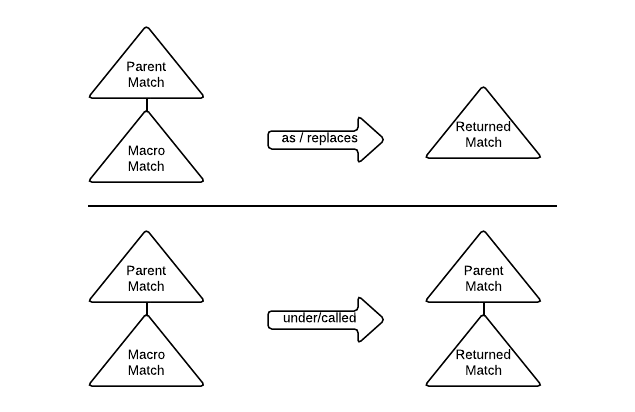
\includegraphics[width=1\textwidth]{img/strats.png}
}
\caption{An illustration of how the different expansion strategies
  work. \texttt{as} differs from \texttt{replaces} by checking that the returned
  match conforms to the parent rule. \texttt{called} differs from \texttt{under}
  by not inserting the macro's rule in the grammar.}
\label{img_strats}
\end{figure}

%%%%%%%%%%%%%%%%%%%%%%%%%%%%%%%%%%%%%%%%%%%%%%%%%%%%%%%%%%%%%%%%%%%%%%%%%%%%%%%%
\subsection{Prioritary Macros}

By default, a macro's rule is inserted as last alternative to its parent
rule. Prioritary macros are instead added as first alternative to their parent
rule. This is sometimes necessary: the only way to write a macro that looks like
a function call is through a prioritary macro.

To make a macro prioritary, add the \texttt{prioritary} keyword right before the
\texttt{macro} keyword, but after the \texttt{raw} keyword, if present.

%%%%%%%%%%%%%%%%%%%%%%%%%%%%%%%%%%%%%%%%%%%%%%%%%%%%%%%%%%%%%%%%%%%%%%%%%%%%%%%%
\section{Working with \texttt{Match}es}
\label{match_api}

This section details the public API of the \texttt{Match} class. Most of the
features relates to finding submatches that fit some criteria.

%%%%%%%%%%%%%%%%%%%%%%%%%%%%%%%%%%%%%%%%%%%%%%%%%%%%%%%%%%%%%%%%%%%%%%%%%%%%%%%%
\subsection{Match Information}

\begin{description}
\item \texttt{originalString()}

  Returns the matched string, exactly like it appeared in the original source.

\item \texttt{string()}

  Returns the matched string, trimmed of leading and trailing
  whitespace. Leading and trailing comments are preserved.

\item \texttt{expression()}

  Returns the \texttt{Expression} this match conforms to.

\item \texttt{children()}

  Returns a \texttt{List<Match>} of the match's children.

\item \texttt{child()}

  Same as \texttt{match.children().get(0)}. Useful when it is known that a match
  has one and only one child.

\item \texttt{empty()}

  Same as \texttt{match.children().isEmpty()}.

\item \texttt{getCaptures(String name)}

  Returns all matches captured with the given name in this match tree, as a
  \texttt{Match[]}. In the body of a macro that has a capture named \texttt{x},
  the variable \texttt{x} is guaranteed to be equivalent to
  \texttt{input.getCaptures("x")}.

  This method is useful to retrieve captures in a rule other than the macro's
  rule.

  If the match this method is called on is itself a capture with the given name,
  it won't be returned.

\end{description}


%%%%%%%%%%%%%%%%%%%%%%%%%%%%%%%%%%%%%%%%%%%%%%%%%%%%%%%%%%%%%%%%%%%%%%%%%%%%%%%%
\subsection{\texttt{MatchSpec}}
\label{matchspec_manual}

A \texttt{MatchSpec} object is a predicate for matches. The
\lstinline{MatchSpec#matches(Match)} method indicates whether the passed match
satisfies the condition expressed by the \texttt{MatchSpec} object.

\texttt{trees.MatchSpec} is actually an abstract class. caxap supplies a few
useful implementation of this class. Each such implementation can be
instantiated either by using its constructor or by using a convenience static
factory method. All implementations are static nested classes of
\texttt{MatchSpec}. All factory methods also belong to \texttt{MatchSpec}.

You can also roll you own implementation of the abstract class.

Here are the supplied implementations. For each we give the signature of its
constructor(s) and the name of the factory method(s). A factory method takes the
same arguments as the associated constructor, and its return type is the
implementing class.

\begin{description}
\item \texttt{StringSpec(String)} / \texttt{rule}

  Matches \texttt{Match} objects for which the result of \texttt{string()}
  equals the supplied string.

\item \texttt{RuleSpec(String)} \& \texttt{RuleSpec(Expression.Rule)} /
  \texttt{rule}

  Matches \texttt{Match} objects for which the result of \texttt{expression()}
  is a rule with the supplied name (\texttt{String} parameter) or with the same
  name as the supplied rule (\texttt{Expression.Rule} parameter).

\item \texttt{ExprSpec(Expression)} / \texttt{expr}

  Matches \texttt{Match} objects for which the result of \texttt{expression()}
  equals the supplied expression.

\item \texttt{OrSpec(MatchSpec...)} / \texttt{or}

  Matches \texttt{Match} object matched by at least one of the supplied specs.

\item \texttt{AndSpec(MatchSpec...)} / \texttt{and}

  Matches \texttt{Match} object matched by all of the supplied specs.

\item \texttt{NotSpec(MatchSpec)} / \texttt{not}

  Matches \texttt{Match} object not matched by the supplied spec.

\item \texttt{HasSpec(MatchSpec)} / \texttt{has}

  Matches \texttt{Match} object which have a descendent that matches the
  supplied spec.

\item \texttt{AnySpec()} / \texttt{anySpec}

  Matches any \texttt{Match} object.

\end{description}

%%%%%%%%%%%%%%%%%%%%%%%%%%%%%%%%%%%%%%%%%%%%%%%%%%%%%%%%%%%%%%%%%%%%%%%%%%%%%%%%
\subsection{Finding Submatches}
\label{finding_submatches}

All methods that search for submatches are passed a \texttt{MatchSpec} as first
parameter. We call it \emph{the main spec}. Only matches fitting this spec can
be returned, although not all fitting matches need to be returned, depending on
the method.

Additionally, one can supply specs for matches that should come to the left or
to the right of the sought matches. We call those specs \emph{left-specs} and
\emph{right-specs}.

We say that a match $A$ is \emph{to the left of} a match $B$ if $A$ is the
descendant of a left-sibling of an ancestor of $B$. A match $A$ comes \emph{to
  the right of} a match $B$ if $A$ is right-sibling of an ancestor of $B$. If
$A$ comes neither to the left or to the right of $B$, meaning one of the two
matches is an ancestor of the other, both matches are said to \emph{overlap}. A
match cannot be at the same time to the left and to the right of another
match. Matches are considered to be ancestors and descendants of themselves.

A depth-first, left-to-right walk of a match tree orders the nodes from left to
right, meaning that no match is visited before all the matches to its left have
been visited, and no match is visited after a match to its right has been
visited. In a depth-first right-to-left walk, nodes are ordered from right to
left. In both cases, all matches are visited, and overlapping matches are
visited in increasing order of depth.

The most general searching methods are \texttt{allBetween(MatchSpec,
  MatchSpec[], MatchSpec[])} and \texttt{allOutside(MatchSpec, MatchSpec[],
  MatchSpec[])}. Those methods return an array of matches. Below we describe the
algorithm used by \texttt{allBetween()}. We then proceed to explain how
\texttt{allOutside()} differs from it, and how all the other searching methods
relate to those two.

\begin{enumerate}

\item Do a depth-first, left-to-right walk of the tree. Test each encountered
  match against the first left-spec. Once a match fits the spec, ignore its
  descendants and test subsequent matches against the second left-spec. Continue
  like this until either all left-specs have been matched, or all the tree nodes
  have been exhausted. In the second case, we stop the algorithm and return the
  empty array. Else we save the location of the match fitting the last left-spec
  (the \emph{left-match}).

\item Do a depth-first, right-to-left walk of the tree. This time we are looking
  for matches fitting the right-specs. Unlike the left-specs, the right-specs
  are iterated from last to first. Like before, if we exhaust the tree nodes, we
  return the empty array, else we save the location of the match fitting the
  first right-spec (the \emph{right-match}).

\item Verify that the right-match comes to the right of the left-match. If not,
  return the empty array.

\item Do a depth-first, left-to-right walk of the tree. Ignore all the matches
  up to the left-match, and all the matches after the right-match. Add all
  encountered matches fitting the main spec to a list of results, and ignore
  their descendants. Return an array containing all the results.

\end{enumerate}

\texttt{allOutside()} works like \texttt{allBetween()}, except that the
left-match is the match fitting the first left-spec and the right-match is the
match fitting the last right-spec (except for the third step). The last step
ignores all nodes between the left-match and the right-match (inclusive). Hence
\emph{outside} instead of \emph{between} in the method name, as that refers to
the parts of the tree where we search for matches fitting the main spec.

The methods \texttt{allAfterFirst(MatchSpec, MatchSpec...)},
\texttt{allBeforeLast(MatchSpec, MatchSpec...)} are like \texttt{allBetween()}
with the second or first array parameter empty, respectively.

Conversely, the methods \texttt{allBeforeFirst(MatchSpec, MatchSpec...)},
\texttt{allAfterLast(MatchSpec, MatchSpec...)} are like \texttt{allOutside()}
with the second or first array parameter empty, respectively.

The method \texttt{all(MatchSpec)} is equivalent to \texttt{allBetween()} with
both array parameters empty. Only the last step is executed, and no matches are
ignored, excepted the descendants of matches fitting the main spec. When both
array parameters to \texttt{allOutside()} are empty, the result is always an
empty array.

All the methods mentioned in this section also have versions in which the words
\texttt{first} or \texttt{last} replace the word \texttt{all} in the method
name. The result of those methods is always equivalent of taking the first or
last item of the array returned by the \texttt{all} version, if not
empty. Otherwise, they returns a value that is recognized by the \texttt{has()}
calls (see next section) as a lack of result.

%%%%%%%%%%%%%%%%%%%%%%%%%%%%%%%%%%%%%%%%%%%%%%%%%%%%%%%%%%%%%%%%%%%%%%%%%%%%%%%%
\subsection{Checking for the Presence of Submatches}

Sometimes, you just want to know whether a match has a submatch fitting a
particular spec. caxap offers three calls towards this end.

\begin{description}

\item \texttt{boolean has(MatchSpec)}

  The simplest one, does as said above.

\item \texttt{boolean has(Match)}

  Takes a \texttt{Match} returned by one of the \texttt{first...()} or
  \texttt{last...()} calls, and checks if the call yielded a result.

\item \texttt{boolean has(Match[])}

  Takes a \texttt{Match} returned by one of the \texttt{all...()} calls, and
  checks if the call yielded some results.

\end{description}

%%%%%%%%%%%%%%%%%%%%%%%%%%%%%%%%%%%%%%%%%%%%%%%%%%%%%%%%%%%%%%%%%%%%%%%%%%%%%%%%
\subsection{Examples}

There are an unlimited amount of ways to combine specs and searching methods to
find matches. Figure \ref{match_finder_examples} shows a few simple examples
extracted from caxap own implementation.

\begin{figure}[here]
\small
\begin{lstlisting}[language=Java, frame=single]
// Get the macro name from its definition.
String ruleName = match.first(rule("identifier")).string();

// Get the macro's parent rule.
String extendedRuleName = match.firstAfterFirst(
    rule("identifier"), rule("strategy")).string();

// Is an unquotation escaped (prefixed by a slash)?
boolean escaped = unquotation.has(
  unquotation.firstBeforeFirst(
    rule("backslash"), or(rule("hash"), rule("hashat"))));
\end{lstlisting}
\caption{Simple examples of submatches finder extracted from caxap
  implementation.}
\label{match_finder_examples}
\end{figure}

%%%%%%%%%%%%%%%%%%%%%%%%%%%%%%%%%%%%%%%%%%%%%%%%%%%%%%%%%%%%%%%%%%%%%%%%%%%%%%%%
\section{(Quasi)quotation}
\label{quotation_manual}

Quotation is one of the basic ways to create new matches in caxap. It is a
process by which we turn some literal source string into a match representing it
as code. Quasiquotation expands on quotation by adding the ability to insert
other fragments of code into our source string.

The design of quasiquotation in caxap follows that of Lisp, with a few
modifications to account for arbitrary syntax. The design of quasiquotation in
Lisp and the evolutions of the concept are thoroughly described in the paper
``Quasiquotation in Lisp''. \cite{quasiquotation}

%%%%%%%%%%%%%%%%%%%%%%%%%%%%%%%%%%%%%%%%%%%%%%%%%%%%%%%%%%%%%%%%%%%%%%%%%%%%%%%%
\subsection{Quotation Basics}
\label{quotation_basics}

\emph{quoting} is the process of turning a character string into a structure
representing code. In our case, this structure is a match tree. Thus quoting is
no different than parsing a source string.

We call \emph{quotation} the application of the \emph{quote} operation. We call
\emph{a quote} the match tree that results from quotation. We use the
\emph{quoted} adjective to refer to the match tree representation of some
code. Quotation takes a source string as input. We call this string \emph{the
  source fragment}.

The example below shows a quoted \texttt{if} statement in caxap. The source
fragment is contained between square brackets. The quotation is delimited by
single quotes. Between the first single quote and square bracket is the name of
the rule used to parse the source fragment (\texttt{expression}).

\begin{lstlisting}
'expression[ if (predicate()) { method(); } ]'
\end{lstlisting}

\emph{Quasiquotation} is similar to quotation, but operates on a source fragment
interspersed with applications of the \emph{unquote} operation
(\emph{unquotation}). The intent of unquotation is to insert some code into a
source fragment. In caxap, said code can be represented by any object, although
we often work with match trees.

The example below shows how to unquote a match for the expression \texttt{42} in
order to obtain a match for the expression \texttt{42 + 52}.

\begin{lstlisting}
Match fortyTwo = 'expression[ 42 ]';
Match sum = `expression[ #fortyTwo + 52 ]`;
\end{lstlisting}

Quasiquotation is delimited by backquotes (\lstinline{`}). The unquotation
operator is the hash symbol (\lstinline{#}). The operator may be followed by any
unary expression, or by another unquotation, which is then said to be nested to
the outer unquotation (see next section). An unary expression is an expression
whose least prioritary operator is not a binary or ternary operator. To use such
operators in conjunction with unquotation, simply wrap the resulting expression
within parentheses. Note that a quotation is a valid unary expression.

The unquotation operand can be any Java object. If it is an instance of
\texttt{Match}, its \texttt{string()} method is used to get the code represented
by the match tree. Otherwise, the \texttt{toString()} method is assumed to
return the represented code.

If the unquotation operand is a match tree, caxap verifies that the unquoted
match tree makes its way to the resulting match tree. This helps avoid scenarios
like this:

\begin{lstlisting}
Match sum = 'expression[ 1 + 1 ]';
Match product = `expression[ #sum * 3 ]`
\end{lstlisting}

\texttt{sum} parses as (1 + 1), whereas \texttt{product} parses as (1 + (1 *
3)), which might not be what we want. The meaning of our code changed because of
the context in which it was inserted.

Admittedly, these checks can be somewhat restrictive. For instance, the
following example won't work because the \texttt{classDeclaration} expected a
\texttt{classBody}, not a \texttt{block}. Normally this is a useful warning: a
class body contains class member declaration and class initializers, whereas a
block contains instructions. Both should not be confused.

\begin{lstlisting}
Match block = 'block [ { int x = 1; } ]';
Match klass = `classDeclaration[ class #block ]`;
\end{lstlisting}

Still, caxap allows you to pull this off very simply should you want it. Simply
convert the match to a string before unquoting it.

\begin{lstlisting}
Match block = 'block [ { int x = 1; } ]';
Match klass = `classDeclaration[ class #block.string() ]`;
\end{lstlisting}

It is also possible to unquote multiple objects at the same time. This is called
splicing and is introduced in section \ref{splicing}.

It may seem that quasiquotation is a generalized form of quotation: quotation is
quasiquotation with no code insertion. Section \ref{non_recur_unquot} shows that
we in fact need both concepts.

We use the terms \emph{quotation}, \emph{quote} and \emph{quoted} to refer to
quotation and quasiquotation both. The context should make clear what is
meant. We sometimes use \emph{simple quotation} to talk about a quotation which
is not a quasiquotation.

Quotations may appear in any source file, not only in macro files. In the
future, I may restrict their use to macro files, unless explicitly requested in
a regular source file.

%%%%%%%%%%%%%%%%%%%%%%%%%%%%%%%%%%%%%%%%%%%%%%%%%%%%%%%%%%%%%%%%%%%%%%%%%%%%%%%%
\subsection{Nested Quotations}
\label{nested_quot}

In addition to being valid operands for unquotations, quotations can also be
quoted. What then should we do in following scenario?

\begin{lstlisting}
`expression[ `expression[ #myExpression ]` ]`
\end{lstlisting}

Assuming \texttt{myExpression} holds a match tree for the code \texttt{1 + 1},
should the returned match tree be for the code \lstinline{`expression[ 1 + 1 ]`}
or for the code \lstinline{`expression[ #myExpression ]`}?

This question shows that we need a way to distinguish unquotations that should
be applied immediately from the ones that should be quoted.

In caxap, the correct answer to the above question is the second one. The
solution to our problem is to use a system of depth. Entering a quasiquotation
(including the top-level one) increases the depth by one, whereas entering an
unquotation decreases it by one. Unquotations entered with a depth of 0 are
applied. Simple quotations do not change the depth, but entering a simple
quotation with depth 0 does prevent the quotations it contains from being
depth-processed.

Figure \ref{quot_ex_one} has an example to help you understand. The arrow
(\texttt{->}) stands for expression evaluation, and \texttt{==} stands for
expression equivalence. The example exhibits the recursive evaluation of an
unquotation's operand: \texttt{y} evaluates to a match tree for \texttt{x},
which itself evaluates to a match tree for \texttt{1}.

\begin{figure}[here]
\small
\begin{lstlisting}[frame=single]
Match x = 'expression[ 1 ]';
Match y = 'expression[ x ]';

   `quotation[ `expression[ ##y ]` ]`
== `quotation[ `expression[ #x ]` ]`
-> `expression[ #x ]`
== `expression[ 1 ]`
-> 1
\end{lstlisting}
\caption{An example that shows the result of recursively evaluating a
  quasiquotation containing nested quotations.}
\label{quot_ex_one}
\end{figure}

While depth-processing a quotation, it is an error if we reach a negative
depth. We always count depth starting at the outermost quotation: nested
quotations are only depth-processed as part of the outermost quotation, never
individually.

Quotations are evaluated within some scope. It is within that scope that the
unquotations with depth 0 are applied. Other unquotations might be applied in
other scopes, if the match tree returned by the quotation gets evaluated in such
a scope. This is typically the case when you compile a match tree to Java code,
then run said Java code. Said otherwise, unquotation operands have a form of
cross-compilation dynamic scope.

%%%%%%%%%%%%%%%%%%%%%%%%%%%%%%%%%%%%%%%%%%%%%%%%%%%%%%%%%%%%%%%%%%%%%%%%%%%%%%%%
\subsection{Non-Recursive Unquotation}
\label{non_recur_unquot}

As you might have noticed, applying a nested unquotation only makes the
innermost unquotation disappear. The unquoted code is still subjected to the
outer unquotations.

Consider then this question. How can obtain a quote for
\lstinline{`expression[ x ]`}, where \texttt{x} is the result of
a method accessible in the current scope?
Consider the following possibilities:

\begin{enumerate}
\item \lstinline{`quotation[ `expression[ ##method() ]` ]`}
\item \lstinline{`quotation[ `expression[ #method() ]` ]`}
\item \lstinline{`quotation[ 'expression[ #method() ]' ]`}
\item \lstinline{`quotation[ 'expression[ #method() ##other() ]' ]`}
\item \lstinline{`quotation[ `expression[ #'expression[ #method() ]' ]` ]`}
\item \lstinline{`quotation[ `expression[ #'expression[x]' ]` ]`}
\end{enumerate}

Item 1 doesn't work: it results in \lstinline{`expression[ #x ]`}. Item 2
doesn't work either: \texttt{method()} is not be evaluated because the
unquotation is entered with depth 1. Item 3 works, but only if the source
fragment does not include other unquotations. This is shown in item 4, which
fails because there is an unquotation with negative depth.

Item 5 is the solution. It is equivalent to item 6. The quotation basically
cancels out the second unquotation by preventing \texttt{x} from being evaluated
later as unquotation operand. After one evaluation, item 4 is therefore
equivalent to \lstinline{`expression[ x ]`}.

This complication is the reason why we need separate notions of quotation and
quasiquotation. The fix exploits the fact that quotation does not increase the
nesting depth.

%%%%%%%%%%%%%%%%%%%%%%%%%%%%%%%%%%%%%%%%%%%%%%%%%%%%%%%%%%%%%%%%%%%%%%%%%%%%%%%%
\subsection{Splicing}
\label{splicing}

Splicing is a variant of unquotation. It allows you to insert an array of
objects in one go. You can specify strings to be inserted before and after the
sequence (unless the sequence is empty), and in-between the items in the
sequence. See the examples in figure \ref{splicing_example}.

\begin{figure}[here]
\small
\begin{lstlisting}[frame=single,language=caxap]
Match[] matches = new Match[] {'expression[ 1 ]', 'expression[ 2 ]'};
Match[] empty   = new Match[] {};

Match args1 = `arguments[ #@ |(|,|)| matches ]`;
Match args2 = `arguments[ ( #@ ||,|| matches ) ]`;

System.out.println(args1.string()); // prints "(1,2)"
System.out.println(args2.string()); // prints "()"
\end{lstlisting}
\caption{caxap code showing example uses of splicing.}
\label{splicing_example}
\end{figure}

The \emph{separators} are enclosed between pipe characters (\texttt{|}). The
first one goes before the sequence, the last one after, and the middle one in
between each item. Any of them can be omitted. If the spliced array is empty,
nothing is inserted.

The spliced object must be an array, but can be any type of array. Each item in
the array is handled as in regular unquotation. This means that even in an
\texttt{Object} array, the code for a \texttt{Match} is obtained by calling its
\texttt{string()} method, and that there are checks to make sure that an
equivalent match makes it to the resulting tree.

If you want to bypass those checks, the static method \texttt{String[]
  Match.strings(Object[])} will convert an array of objects to an array of
\texttt{String} for you. This array can then be spliced with equivalent results
as splicing the original array, except for the checks.

See section \ref{quotation_basics} for all the details about regular
unquotation.

%%%%%%%%%%%%%%%%%%%%%%%%%%%%%%%%%%%%%%%%%%%%%%%%%%%%%%%%%%%%%%%%%%%%%%%%%%%%%%%%
\subsection{Quotation \& Escaped Sequences}

We have now seen all syntaxes for quotation. Those syntaxes are delimited by
some special characters or character sequences. This means there are places
where you can't use those characters or sequences. You can however substitute
them with the escaped sequences described in this section.

In both regular quotations and quasiquotations, the sequences \lstinline{]'} and
\lstinline{]`} cannot appear. They can however appear as part of a unary
expression which is part of an unquotation, and should not be escaped there. To
escape those sequences, simply prefix them with a backslash (\lstinline{\}). If
  you want to end your source fragment by a backslash, you should make sure that
  your rule allows trailing whitespace, and put some whitespace between your
  backslash and the closing square bracket. In the base Java grammar, all rules
  that can end with a backslash allow trailing whitespace.

  The hash character can also be escaped inside quotations by prefixing it with
  a backslash: \lstinline{\#}. To have an unquotation preceded by a backslash,
  use the whitespace trick mentioned above: \lstinline{\ #}.

  Note that those escapes must appear even in unlikely places, such as string
  literals. You however never have to worry about escaping a Match that is
  handed to you from some other source. You only have to worry about escaping
  when writing things inside the brackets of the quotation syntax.

  When using the splice operator, you can escape the pipe character with
  \lstinline{\|}. The backslash character must itself be escaped:
  \lstinline{\\}. We also support some additional escapes for convenience:
  \lstinline{\t} for tabulation, \lstinline{\n} for newline, and \lstinline{\r}
  for carriage return. For implementation reasons, other backslash-prefixed
  escapes might also work, but there is no guarantee that they will remain
  supported. There are not needed anyway.

  Finally, it should be noted that it is not possible to use quasiquotation to
  quote some code with significant leading whitespace: that whitespace gets
  consumed by the \texttt{[} token in the quotation syntax. Note that whitespace
  includes comments. There is a workaround: just output the whitespace to a
  string, and unquote that string at the begin of the quotation (make it a
  quasiquotation if needed). This workaround is demonstrated in the file
  \texttt{examples/src/pkg/Comments.javam}.

%%%%%%%%%%%%%%%%%%%%%%%%%%%%%%%%%%%%%%%%%%%%%%%%%%%%%%%%%%%%%%%%%%%%%%%%%%%%%%%%
\section{Macro Composition}

Up to this point, we have explained how macros work in isolation. This section
examines how macros can interact with each other.

%%%%%%%%%%%%%%%%%%%%%%%%%%%%%%%%%%%%%%%%%%%%%%%%%%%%%%%%%%%%%%%%%%%%%%%%%%%%%%%%
\subsection{Composing Unrelated Macros}

% TODO until

Consider the \texttt{Unless} macro from figure \ref{simple_macro_example} and
the \texttt{Until} macro from figure \ref{until_macro}. Each macro has
\texttt{statement} as parent rule, and can have statements as submatches, via
the \texttt{block} rule. caxap naturally allows an \texttt{Unless} match to be a
submatch of an \texttt{Until} match, and vice-versa. In fact an \texttt{Until}
match can perfectly be a submatch of another \texttt{Until} match. The point is
illustrated in figure \ref{composition_example}.

\begin{figure}[here]
\small
\begin{lstlisting}[frame=single,language=caxap]
macro Until as statement
: "until" expr:expression :block {
  return `statement[ while (!(#expr[0])) #block[0] ]`;
}
\end{lstlisting}
\caption{caxap code defining an \emph{until} construct (a while loop with a
  negated condition) as a macro.}
\label{until_macro}
\end{figure}

\begin{figure}[here]
\small
\begin{lstlisting}[frame=single,language=Java]
int i = 0;
until i == 10 {
  unless i % 2 == 0 {
    System.out.println(i);
  }
}
\end{lstlisting}
\caption{Composing the \texttt{Unless} and \texttt{Until} macros. The code
  prints all odd number between 0 and 10.}
\label{composition_example}
\end{figure}

Because arbitrary code can be run to generate a macro's expansion, it cannot be
guaranteed that all macros can be freely composed. Macro implementers should be
loath to introduce such incompatibilities, and if they really have to, should
clearly document them.

%%%%%%%%%%%%%%%%%%%%%%%%%%%%%%%%%%%%%%%%%%%%%%%%%%%%%%%%%%%%%%%%%%%%%%%%%%%%%%%%
\subsection{Macro Expansion Order \& Raw Macros}
\label{raw_macros}

Macros are expanded bottom-up. This means that in figure
\ref{composition_example}, the \texttt{Unless} macro call will be expanded
before the \texttt{Until} macro call.

In the case of figure \ref{composition_example}, this distinction is irrelevant:
since the statements submatches are copied to the output, the \texttt{Unless}
macro call would have been expanded after the \texttt{Until} call if macros
weren't expanded bottom-up (because of recursive expansion, as explained in
section \ref{macro_expansion_intro}).

Sometimes order matters, or you don't want a macro to expand to all.  In those
cases, you can use \emph{raw macros}. A raw macro is a macro whose macro
submatches are not expanded. You can then pass them on to the output, which will
cause them to expand, or just ignore them. You make a macro raw by prefixing its
definition with the \texttt{raw} keyword.

%%%%%%%%%%%%%%%%%%%%%%%%%%%%%%%%%%%%%%%%%%%%%%%%%%%%%%%%%%%%%%%%%%%%%%%%%%%%%%%%
\subsection{Macros Referencing Macros}
\label{noop_macros}

A macro's syntactic declaration can contain direct references to other macros'
rules - or in fact, to their own rule - as long as those rule use the
\texttt{called} expansion strategy. This is currently not enforced by caxap: the
checks need to be implemented. The macros must have been required - or defined
earlier in the same file - in order to be referencable.

For macro with the \texttt{called} strategy, you can elect to replace the macro
body by a semicolon. The resulting macros are called \emph{no-op macros} and do
not expand: the match is preserved as though it was under a raw macro. This
allows you to define reusable syntactic elements.

A macro's parent rule can also be another macro's rule. Albeit we do not
currently restrict this, extending a macro which is not no-op is fraught with
peril. You risk causing an error in the parent macro's expansion code, which
more than likely references the matched input.

%%%%%%%%%%%%%%%%%%%%%%%%%%%%%%%%%%%%%%%%%%%%%%%%%%%%%%%%%%%%%%%%%%%%%%%%%%%%%%%%
\section{Error Reporting}
\label{error_reporting_manual}

Error reporting in caxap is currently in a poor state. In case of error, you
should in principle get a message describing exactly what went wrong and caused
caxap to abort, but the details may sometimes be vague. You'll also get a nice
Java stack trace for free.

Currently, most errors are implemented as unchecked exception that bubble up to
the top of the call stack. In the future, I plan to consolidate all the
exceptions in a well thought-out hierarchy.

A special note on syntax errors: arbitrary syntax makes them especially
difficult to get right.

Parse errors are normal during PEG parsing: they simply mean that we should try
the next alternative of an ancestor of the failing expression. When all possible
alternatives fail, the whole parse fails and we should report a syntax error.

The current strategy is to keep track of the farthest input position causing an
error. Once there are no more alternatives to try, we report all errors at that
farthest input position.

Surprisingly, there can be quite a few different errors happening at the same
input position, and caxap currently display the ancestry of all of them. This
can make the output of a parse error quite unwieldy.

caxap already has some tricks to lessen the information overload. For instance,
if a rule fails without matching any character, only the name of that rule is
reported, and not all of its alternatives, which by definition also failed.

Error reporting for grammars which are not fixed in advance is known to be a
hard problem, and other generic PEG parsers such as Parboiled \cite{parboiled}
or Mouse \cite{redziejowski2009} don't do better than caxap in this regard.

%%%%%%%%%%%%%%%%%%%%%%%%%%%%%%%%%%%%%%%%%%%%%%%%%%%%%%%%%%%%%%%%%%%%%%%%%%%%%%%%
\section{Miscellaneous Concerns}

If you choose to reference the grammar rule for macro definition
(\texttt{macroDefinition}) from your own macro, you must make sure that if a
macro definition is parsed, it will make it to the final match tree. The reason
for this constraint is explained in section \ref{implem_grammar}.

You can use caxap's API in your regular programs (i.e. outside of macros). But
if you do so, you need to make sure that caxap's jar file appears on the
classpath of your program.

A common pattern in macro development is to factor out some common logic between
macros to an external class. Unfortunately this class will be expanded and
copied to the output directory like the rest. When you try to compile it, Java
will serve you an error if caxap is not on your classpath. This will be fixed in
a future release.

\chapter{Implementation \& Internals}

In this section, we look at what caxap has under the hood. We start with an
overview of the whole implementation, and then linger on a few topics that were
tricky to implement and/or design.

This chapter assumes you have read - and hopefully understood - the user manual
(chapter \ref{manual}).

%%%%%%%%%%%%%%%%%%%%%%%%%%%%%%%%%%%%%%%%%%%%%%%%%%%%%%%%%%%%%%%%%%%%%%%%%%%%%%%%
\section{Overview of the Architecture}

In this section, we briefly describe how caxap is implemented. We do so by
giving a cursory overview of each package in the caxap source tree.

%%%%%%%%%%%%%%%%%%%%%%%%%%%%%%%%%%%%%%%%
\subsection{driver}

The \texttt{EntryPoint} class is - unsurprisingly - caxap's entry point. It
processes command line options and makes them available to other parts of the
program via the singleton \texttt{Config} class. It then finds all source files
and uses the \texttt{DependencyResolver} class to order them. Finally, it passes
control to the class \texttt{CompilationDriver} which will proceed to compile
and/or expand the files in the given order.

The \texttt{CompilationDriver} has ties to the \texttt{compiler.java} package,
in order to compile expanded sources and load them in caxap's JVM.

The class \texttt{SourceFile} models each found source file. Each instance of
\texttt{SourceFile} uniquely identifies a source file. All instances of this
class must be obtained via the \texttt{SourceRepository} class, which enforces
the one-to-one mapping between \texttt{SourceFile} instances and files.

Each \texttt{SourceFile} maintains a list of the macros it defines, as well as a
list of dependencies under the form of a \texttt{Requires} object. Each instance
also has its own \texttt{SourceParseManager} which calls into the
\texttt{parser} package to parse either the file prelude or the whole file. The
file prelude consists of the package declaration and of the
\texttt{import}/\texttt{require} statements. Parsing the prelude is actually
delegated to the \texttt{RequiresParser} class.

The \texttt{Context} class makes some data globally accessible to avoid passing
it over the call stack, or to let callbacks manipulate it.

The \texttt{Hints} class is an early attempt to provide better diagnostics by
providing some context that can be used in error messages.

%%%%%%%%%%%%%%%%%%%%%%%%%%%%%%%%%%%%%%%%
\subsection{files}

Classes in this package model source files on the disk and how they relate with
the package structure. The \texttt{Require} class models as ingle
\texttt{require} statement. These classes are mostly used in the \texttt{driver}
package.

%%%%%%%%%%%%%%%%%%%%%%%%%%%%%%%%%%%%%%%%
\subsection{grammar}
\label{implem_grammar}

\texttt{Expression} is the most important class in this package. It models a PEG
parsing expression. There is one nested class per type of expression.

The base grammar for Java is defined in the \texttt{grammar.java} package, using
a domain specific language (DSL) defined in \texttt{GrammarDSL}.

In PEG, expressions form graphs, not trees, because of recursion. Building a
graph in one step is tricky in Java, since you can't use a uninitialized
variable in its definition. For instance you can't write:

\begin{lstlisting}
Expression arguments = rule_seq(identifier, opt(comma, arguments));
\end{lstlisting}

You have to use an explicit reference instead:

\begin{lstlisting}
Expression arguments = rule_seq(identifier, opt(comma, ref("arguments"));
\end{lstlisting}

Such references then have to be resolved. This is, among other things, the role
of the \texttt{ExpressionTreeCleaner} class. It also computes a textual
representation for the expression, using the notation introduced in sections
\ref{peg_formalism} and \ref{extended_notation}. Finally, it compacts the graph
by merging identical expressions. This serves to make memoization more
efficient.

The \texttt{Grammar} class represents a PEG grammar. Its constructor takes a
class as parameter (such as those in the \texttt{grammar.java} package), and
uses reflection to get the rule names from the field names. A grammar keeps a
map from rule names to the corresponding \texttt{Expression}.

The \texttt{ExpressionVisitor} interface is simply a programming trick that
allows the implementing classes to specialize some behavior depending on the
run-time type of an object with static type \texttt{Expression}. Calling
\texttt{expression.accept(visitor)} will call the appropriate \texttt{visit()}
method depending on the expression type.

The \texttt{MatchCallbacks} class defines a number of methods called on a
\texttt{Match} object at different time during its lifetime: when it is
constructed during the parse, before and after macro expansion.

Callbacks are used to implement some important features, such as compiling and
registering macro definitions. This means that that if a macro definitions is
parsed, it must make it to the final match tree, because there is no way to
unregister a macro if the parser backtracks over the macro definition.

Albeit the feature is not documented, it is possible for users to define their
own callbacks. In the future, I hope to add some new syntax and functionalities
to make the feature more transparent.

The \texttt{Expression} and \texttt{ExpressionVisitor} classes are heavily
inspired by similar classes written by Roman R. Redziejowski for the Mouse PEG
parser generator. \cite{redziejowski2009}

%%%%%%%%%%%%%%%%%%%%%%%%%%%%%%%%%%%%%%%%
\subsection{source}

The \texttt{Source} interface describes a container of source code. The
\texttt{SourceStream} class associates a \texttt{Source} object with position
within that source. Each instance of our parser class is associated to a
\texttt{Source} object, and uses a \texttt{SourceStream} to keep track of its
position in the source.

The package also contains a few implementation of the \texttt{Source}
interface. \texttt{SourceFileText} represents a source file whose contents have
been read into memory. \texttt{SourceString} represents code contained in a Java
string. \texttt{SourceComposed} represents code pieced together to support the
\texttt{MatchCreator.new_match()} methods described in section
\ref{match_class}.

The \texttt{Source} interface and most of the implementing classes were
originally written by Roman R. Redziejowski for the Mouse PEG parser
\cite{redziejowski2009}. I only made minor adaptations to his code.

%%%%%%%%%%%%%%%%%%%%%%%%%%%%%%%%%%%%%%%%
\subsection{grammar.java}

The package comprises five special files starting with the
\texttt{_<uppercase-leter>_} pattern. The fields in those classes represent the
rules of the base Java grammar. The grammar was so large that it was indeed
preferable to split it across multiple files. The lexical ordering hints at the
inheritance hierarchy: E extends D extends C ...

\texttt{JavaGrammar} extends the E class. The base Java grammar is obtained by
passing \texttt{JavaGrammar.class} to the constructor of the
\texttt{grammar.Grammar} class.

The remaining classes are \texttt{grammar.MatchCallbacks} implementations.

\texttt{CallbacksExpression} builds \texttt{Expression} objects from a macro's
syntactic specification. I hesitated to implement the features as a form of
bootstrapped macro instead.

\texttt{CallbacksMacroDefinition} handles the compilation and registration of a
macro right after its definition has been parsed.

\texttt{CallbacksPrelude} expands \texttt{require} statements into
\texttt{import} statements, or swallows them, in the case of macro requires. In
practice, it does not really expand anything but rather replaces all
\texttt{import} and \texttt{require} statements with a list of \texttt{import}
statement that was computed when the file prelude was first parsed.

%%%%%%%%%%%%%%%%%%%%%%%%%%%%%%%%%%%%%%%%
\subsection{parser}

This package holds the implementation of our PEG parser.

The \texttt{Match} class is described in details in sections \ref{match_class}
and \ref{match_api} of the user manual.

The core of the parser is in the \texttt{Matcher} class. Its constructor takes
an instance of \texttt{source.Source} and wraps it in a
\texttt{source.SourceStream}, which can then be used to find a \texttt{Match}
for a given \texttt{Expression} at the current position in the source.

We tried to keep the code clean, but there is nothing particularly fancy about
the implementation: we use the memoized depth-first walk of the expression graph
which is typical of packrat parsers (see section \ref{packrat_parsing} or
\cite{ford2002}). Memoization is handled by the \texttt{Memo} class. For each
rule it has to parse, the parser calls the method \texttt{Memo\#get(int position,
  Expression expr)}. That method either returns a memoized \texttt{ParseData}
object; either calls back into \texttt{Matcher} to get such an object, which is
then memoized and returned.

\texttt{Memo} is actually an interface. We supply three implementations of it,
that each represents a different memoization strategy or implementation. Those
are \texttt{NestedMemo}, \texttt{FlatMemo} and \texttt{LimitedMemo}. They are
described in section \ref{implem_perf}.

\texttt{Matcher} implements \texttt{grammar.ExpressionVisitor} in order to parse
each expression according to its specificities.

Each time the matcher attempts to find an expression match at a given position
in the source file, a \texttt{ParseData} object is created if none have been
memoized. This object records whether the match was successful. If it was, it
holds the corresponding \texttt{Match} object. In all cases, it also holds a
\texttt{ParseErrors} object containing the encountered parse errors. The error
reporting strategy is described in section \ref{error_reporting_manual}.

We need the \texttt{ParseData} class in addition to the \texttt{Match} class,
because \texttt{Match} is not designed to hold temporary information needed
while parsing. In particular, in case of match failure, we need to record the
failure and its cause. This is important, because failing to match an expression
can be explained by failing to match one of its sub-expressions.

Regardless of the result of an expression match, its \texttt{ParseData} is
merged into the \texttt{ParseData} of its parent: this registers a sub-match in
case of success, and merges error information.

%%%%%%%%%%%%%%%%%%%%%%%%%%%%%%%%%%%%%%%%
\subsection{trees}

The \texttt{MatchSpec} class is described in section \ref{matchspec_manual}.

The \texttt{MatchFinder} class is the implementation backbone of the
match-finding methods described in section \ref{finding_submatches}.

\texttt{MatchIterator} and \texttt{BoundedMatchIterator} are two iterator
implementations used in \texttt{MatchFinder}. \texttt{MatchIterator} simply
iterates on a match tree depth-first, either left-to-right or
right-to-left. \texttt{BoundedMatchIterator} encapsulates a
\texttt{MatchIterator} but only returns the nodes between or outside the
\emph{left-match} and \emph{right-match} (as described in section
\ref{finding_submatches}).

%%%%%%%%%%%%%%%%%%%%%%%%%%%%%%%%%%%%%%%%
\subsection{compiler}
\label{compiler_tour}

This package concerns itself with the compilation of macros and the expansion of
macro calls.

The \texttt{Macro} class holds all attributes of a macro, as described in the
user manual.

The \texttt{MacroCompiler} class is responsible for turning a macro into
compiled bytecode. It requires three key pieces of information: the macro name,
the expanded macro body, and the list of \texttt{import} statements that should
be included in the compiled source (derived from the macro file prelude).

The \texttt{compiler.java} package is used to turn the source pieced from these
pieces of information into bytecode.

A match tree is an immutable structure. The \texttt{MatchTreeTransformer}
abstract class holds the logic to apply a recursive transformation on a match
tree, and rebuild only the parts of the tree which have changed. The subtrees
that have not changed are shared between the new and the old tree. Implementing
classes just need to implement a method that transforms a single \texttt{Match}.

There are three classes implementing \texttt{MatchTreeTransformer}. The
\texttt{MacroExpander} class expands encountered macros according to their
expansion strategies, as described in section \ref{expansion_strategies} (see
also sections \ref{macro_expansion_intro} and \ref{raw_macros} on macro
expansion).

The \texttt{PostParseTransformer} and \texttt{PostExpansionTransformer} classes
from the \texttt{CallbacksTransformers.java} file apply the transformations that
result from some of the callbacks specified in \texttt{MatchCallbacks} objects.

The \texttt{PostParser} class simply applies the transformations from
\texttt{PostParseTransformer}, \texttt{MacroExpander} and
\texttt{PostExpansionTransformer}, in that order.

Finally, the \texttt{QuotationMacro} class is a bootstrapped macro that expands
the quotation syntax (see section \ref{quotation_manual}) into calls to Java
methods defined in the \texttt{compiler.util.Quoter} class. We say
\emph{bootstrapped} macro, because, while it acts exactly like a macro, it was
hand-coded and not compiled via \texttt{MacroCompiler}.

%%%%%%%%%%%%%%%%%%%%%%%%%%%%%%%%%%%%%%%%
\subsection{compiler.java}

The classes in this package interface with the \texttt{javax.tools} package from
the JDK libraries. \texttt{DynamicJavaCompiler} defines our own interface to the
compiler, which takes \texttt{javax.tools.JavaFileObject} instances and returns
a list of \texttt{CompiledClass} instances (one per class defined in the file
objects).

The \texttt{javax.tools.JavaFileObject} class represents a Java compilation
unit, meaning a source file. The \texttt{CompiledClass} class represents the
bytecode obtained by compiling a Java class.

The \texttt{StringJavaFileObject} class extends the
\texttt{javax.tools.JavaFileObject} class to allow us to use strings as the
source code of compilation units.

Finally, the \texttt{MemoryClassLoader} is a class loader that can hold the
bytecode of classes in memory. When searching for a class to load, it will first
search among the classes whose bytecode is in memory, then only search for
\texttt{.class} files on the disk.

%%%%%%%%%%%%%%%%%%%%%%%%%%%%%%%%%%%%%%%%
\subsection{compiler.util}

The facilities in \texttt{MatchCreator} are described in section
\ref{match_class}.

The \texttt{StringMatcher} class holds a small helper method that abstracts away
the boilerplate needed to match a source string to a grammar rule.

The class \texttt{PEGCompiler} takes a string representing a macro's syntactic
specification and returns the corresponding \texttt{Expression}. This is
currently unused except in tests.

Last but not least, the \texttt{Quoter} class implements the quotation
primitives. The way this class relates to quotation as described in the manual
is explained in section \ref{implem_quotations}.

%%%%%%%%%%%%%%%%%%%%%%%%%%%%%%%%%%%%%%%%
\subsection{compiler.macros}

This is the package in which compiled macros will be placed. It only contains
the \texttt{MacroInterface} interface, which is the interface that the class
generated for each macro must implement.

%%%%%%%%%%%%%%%%%%%%%%%%%%%%%%%%%%%%%%%%
\subsection{util and util.apache}

The package holds a collection of data structures and utilities that ease some
programming tasks, but are not inherently tied to our program's logic.

\texttt{util.apache} has classes extracted from the Apache Commons library. In
particular, they deal with source code escaping.

%%%%%%%%%%%%%%%%%%%%%%%%%%%%%%%%%%%%%%%%%%%%%%%%%%%%%%%%%%%%%%%%%%%%%%%%%%%%%%%%
\section{The \texttt{require} Statement}

Introduced in section \ref{require_manual} of the user manual, the
\texttt{require} statement extends the functionality of the \texttt{import}
statement by explicitly specifying which source file is being depended upon.

Central to understanding the \texttt{require} statement is the notion of
\emph{dependency}, and the difference between a run-time and compile-time
dependency. We first describe see how Java handles dependencies before
explaining how caxap deals with dependencies at compile time.

%%%%%%%%%%%%%%%%%%%%%%%%%%%%%%%%%%%%%%%%%%%%%%%%%%%%%%%%%%%%%%%%%%%%%%%%%%%%%%%%
\subsection{Dependencies and the Java Compiler}

We describe here how dependencies are handled in Java. This helps explaining why
we needed to introduce \texttt{require} statements instead of hijacking the Java
\texttt{import} statement.

We base our discussion on the Oracle Java compiler (\emph{javac}), but most
things are applicable to all Java compilers targeting the Java Virtual Machine
(JVM).

%%%%%%%%%%%%%%%%%%%%%%%%%%%%%%%%%%%%%%%%%%%%%%%%%%%%%%%%%%%%%%%%%%%%%%%%%%%%%%%%
\subsubsection{Dependencies and \texttt{import} Statements}

The first and foremost thing to understand is that, in Java, the dependencies of
a class are the set of other classes referenced in the class.

As most people will tell you, \texttt{import} statements are related to
dependencies. What most people don't realize however, is that, in Java,
\texttt{import} statement are merely a convenience to avoid using the fully
qualified name of each class (e.g. using \texttt{List} instead of
\texttt{java.util.List}). Every \texttt{import} statement in Java could be
removed at the cost of verbosity. This would not change the class dependencies.

There are two kinds of \texttt{import} statements in Java. Regular
\texttt{import} statements import a class name from another package. Static
imports - denoted by the keyword \texttt{static} - import the name of a static
method, field or class from another class. Both kind can also end with a
wildcard (\lstinline{'*'}) rather than a name. In that case all classes in the
package or static members in the class are imported.

When javac encounters an identifier that could potentially be a class name,
javac will attempt to resolve the identifier as a class in the same package as
the class being compiled. This means that all classes from the same package are
implicitly imported in every class.

%%%%%%%%%%%%%%%%%%%%%%%%%%%%%%%%%%%%%%%%%%%%%%%%%%%%%%%%%%%%%%%%%%%%%%%%%%%%%%%%
\subsubsection{Dependencies at Compile Time and Run Time}

While dependencies are checked by the compiler at compile time, the result of
compilation is a set of \texttt{.class} file containing bytecode. There is one
\texttt{.class} file per class defined in the source file(s). This means that
the JVM must resolve the dependencies at run time, much like how dynamically
linked library work. The JVM does this by looking for the appropriate
\texttt{.class} file on the classpath. The classpath is a list of paths where
the compiler looks for \texttt{.class} files. The user can add paths to the
classpath using the command line options of the JVM.

The compiler, which takes a set of source file as input, checks the dependencies
of those files at compile time. For each import statement, the compiler ensures
that the imported classes or class members are defined. The compiler looks for
those in two places. First, inside \texttt{.class} files which are found on the
classpath. The compiler also looks for definitions in the source files
themselves, since the relevant source file might not have been compiled to
\texttt{.class} files yet.

Since a single source file can contain the definition of multiple classes, there
can be more than one \texttt{.class} file emitted for each source file.

%%%%%%%%%%%%%%%%%%%%%%%%%%%%%%%%%%%%%%%%%%%%%%%%%%%%%%%%%%%%%%%%%%%%%%%%%%%%%%%%
\subsection{Problems with the \texttt{import} Statements}
\label{import_problems}

We can't use \texttt{import} statements to specify dependencies between source
files. First, the aim of \texttt{import} statement is not to specify
dependencies, but to avoid typing out the fully qualified name of each class
each time it is used. Second, \texttt{import} statements reference
classes. There is an asymmetry between classes and source files: a source file
can contain the definition of multiples classes.

The fully qualified class names used in \texttt{import} statements are also
ambiguous with regard to the location of the containing source file. Consider
the statement ``\texttt{import com.company.project.Class;}''. The class
\texttt{Class} could simply be defined in the file
\texttt{com/company/project/Class.java}. The class could also be defined in any
other file in the package, if it isn't public. Worse, it could be defined inside
the file \texttt{com/company/project.java}, if \texttt{Class} is a nested class
of the class \texttt{project}. While convention dictates that class names begin
with an uppercase letter, this is not enforced by the Java compiler.

Even if we were willing to find the file in which a class was defined, it would
prove to be impossible in the presence of macros. Indeed, a macro call could
``hide'' the class definition, and we cannot expand macros before resolving
dependencies.

Clearly, a new syntax was required to deal with source file dependencies.

%%%%%%%%%%%%%%%%%%%%%%%%%%%%%%%%%%%%%%%%%%%%%%%%%%%%%%%%%%%%%%%%%%%%%%%%%%%%%%%%
\subsection{Why do we need compile-time dependencies?}
\label{why_source_deps}

As explained in section \ref{require_manual}, we must know of dependencies
between source files so that we can find a linear ordering of source files. We
then compile the files in that order.

If a source file uses a macro, then the macro's expansion code needs to be
compiled before the source file can be compiled. This automatically precludes
cyclic dependencies between macros: When trying to compile a macro's expansion
code, we would need the compiled expansion code of another macro, the
compilation of which would need the compiled expansion code of the macro we were
trying to compile in the first place.

But wouldn't it still be possible to have cyclic dependencies between macro
files, as long as there are no cyclic dependencies between macros? The problem
is that since a macro body can contain macro calls, we can only know where the
macro body ends after having seen the syntactic specification of the macros it
calls. But we can't know in advance which macros the body calls; hence we need
to see all required macros syntactic specification, and thus parse all required
macros' bodies.

There are a few ways around this. We could specify the macro depended upon at
the macro definition level. We could move all syntactic specifications to the
top of the file. Or we could reserve a token to indicate the end of a macro's
body, which could not be used in user-defined syntax. All those fixes seem to be
more bothersome than they are worth.

If a macro file uses a class in its expansion code, then this class needs to be
located by the Java compiler. This means that the compiler must have access to a
\texttt{.class} for the macro, or to a source file containing its definition. In
the second case, we still need to fully pre-process the defining source file;
hence there is still a dependency link.

Dependencies between two regular source files need to be specified for two
reasons. The first is that they can lead to a transitive dependency on a
macro. Let A, B be regular source files, and C a macro file. If a A depends on B
and B depends on C, then C must be compiled before A can be compiled.

Second, caxap compiles files only if they are somehow required for macro
expansion. If we did not specify a dependency on another source file, we would
not know we need to compile it.

Currently, files are compiled one at a time. This forbids some well-behaved
cases such as the following example. Let A, B be regular source files containing
no macro calls, and C a macro file. C depends on A, A depends on B and B depends
on A. There is a cyclic dependency between A and B that will be rejected by
caxap. Yet, this dependency could be encoded using \texttt{import} statement and
would compile just fine if we supplied both A and B to the Java compiler.

In the future, we might try to produce some kind partial ordering that would
allow us to compile multiple files together, instead of a total ordering.

%%%%%%%%%%%%%%%%%%%%%%%%%%%%%%%%%%%%%%%%%%%%%%%%%%%%%%%%%%%%%%%%%%%%%%%%%%%%%%%%
\section{Finding Submatches}

The design of the match finding API described in section \ref{match_api} is
pretty interesting. I wanted to make an API that would make it easy to retrieve
submatches in a match tree, without needing to refer back to the grammar
constantly.

The goal of the API is to be able to express the position of a match in the
exact same way as people think about it. It turns out that if you want to
describe the location of a match, you'll probably anchor your description to
some element that precedes or follows that match. You'll use words such as
\emph{after}, \emph{before} or \emph{between}. If multiple matches satisfy the
requirements, these prepositions will typically be complemented by words such as
\emph{first} or \emph{last}.

This explains the overall structure of the API, particularly its
\emph{first}/\emph{last}/\emph{all} and
\emph{after}/\emph{before}/\emph{between}/\emph{outside} distinctions.

Moreover, the variety of available \texttt{MachSpec} (see section
\ref{matchspec_manual}) allows specifying matches even if the exact name of the
grammar rule is not known. You can express conjunction and disjunction of specs
with \texttt{AndSpec} and or \texttt{OrSpec}. And of course, if something is
missing, you can always roll your own \texttt{MatchSpec} implementation.

In our experience - which is at present somewhat limited - the system succeeds
at making most request terse and intuitive. The approach does have a drawback in
that it is not overly efficient, since it is basically a tree search.

The idea of finding data in an annotated tree is not a new idea. In fact, it is
rather pervasive: the cascading stylesheet language (CSS) \cite{css_page} used
on almost every website is constructed around this idea. CSS tries to match HTML
tags to apply styling on them. CSS uses the term \emph{selector} instead of
\emph{specification}.

There are differences however. First, CSS is skewed toward matching potentially
large set of scattered items, whereas we tend to more stringent in our
requirements. Unique HTML tags in a page layout are given a unique \emph{id},
which further simplifies CSS' task. Another difference is that CSS match items
recursively, which makes sense in its context.

There are other query languages operating on trees that work somewhat
similarly. One example is the XPath query language \cite{xpath}, which is part
of the XSLT (Extensible Stylesheet Language Transformations) language.

%%%%%%%%%%%%%%%%%%%%%%%%%%%%%%%%%%%%%%%%%%%%%%%%%%%%%%%%%%%%%%%%%%%%%%%%%%%%%%%%
\section{Quotations}
\label{implem_quotations}

The most difficult thing about quotations is understanding how they work. After
that, implementing them is not all that hard, if you get the right ideas.

As mentioned in section \ref{compiler_tour}, the quotation syntax acts like a
macro, implemented in \texttt{compiler.QuotationMacro}.

Simple quotations expand to the \texttt{compiler.util.Quoter.primitiveQuote()}
method. For instance, \lstinline{'expression[ 42 ]'} expands to
\texttt{primitiveQuote("expression", "42")}. The first parameter is a rule name,
and the second is the source fragment, escaped so as to form a valid Java
string.

\texttt{primitiveQuote()}, which is overloaded, can also take a list of
\texttt{MatchSpec} objects as a list or as a variadic parameter. The method
checks if the match resulting from the quotation satisfies all passed
specs. This parameter is not used for simple quotations.

Quasiquotations expand to the \texttt{compiler.util.Quoter.dynamicQuote()}
method. For instance, \lstinline{`expression[ 1337 + #method() ]`} expands to
\lstinline{dynamicQuote("expression", "1337 + #1", method())}. The reformulation
is necessary in order to evaluate unquoted expression in Java. The
\texttt{dynamicQuote()} method inserts the result of all unquoted expressions
into the source fragment, before passing it to \texttt{primitiveQuote()}. If the
unquoted expression is a \texttt{Match}, \texttt{dynamicQuote()} also constructs
a special \texttt{MatchSpec} instance that ensures that the match appears as a
submatch in the quotation's result, and passes this spec to
\texttt{primitiveQuote()}.

%%%%%%%%%%%%%%%%%%%%%%%%%%%%%%%%%%%%%%%%%%%%%%%%%%%%%%%%%%%%%%%%%%%%%%%%%%%%%%%%
\section{The Java Grammar}
\label{our_java_grammar}

The PEG grammar used to parse the Java language is entirely hand crafted. There
are a few PEG grammars for Java to be found online, namely as part of the
Parboiled \cite{parboiled}, Mouse \cite{redziejowski2009} and Rats!
\cite{grimm2006} PEG parsers. None truly satisfied me: The Parboiled grammar was
for Java 6; the Rats! grammar used a copious amount of Rats! specific extensions
and both the Mouse and Parboiled grammars was based upon the CFG grammar from
the Java Language Specification \cite{jls} which is explicitly designed to
minimize lookahead. I also found a few errors in the Mouse grammar, which is the
only grammar I thoroughly scrutinized.

My idea for the perfect Java grammar was that it should reflect how one thinks
about the language. In other words, the grammar should map cleanly to our
intuitions about the language. It should also be highly granular: since each
rule is a potential macro insertion point, there should be enough rules to
capture all the places where a user might want to insert a macro, and the rules
should represent meaningful Java entities. There should not be too large a
divide between the syntactic and semantic view of the language.

Unfortunately, grammars designed to minimize lookahead violate those principles,
notably by \emph{factoring out} common prefixes of rules. This means that we are
left with very grave gaps: there are for instance no rule that designate array
access or method invocation directly. Instead, we have a rule with an identifier
as prefix, which is followed by any number of suffixes such as array access or
method invocations. In the context of our macro system, that does constitute a
problem.

Yet, my grammar is not devoid of problems. First, it ended up picking some of
the gaps highlighted above because the PEG formalism does not support left
recursion. While we can emulate left-recursion using the ``prefix followed by a
repetition of suffixes'' pattern, left-recursion produces a nesting of rules
that properly associates each array access / method invocation with its prefix
operand. As explained in section \ref{peg_left_recursion}, there are ways to
introduce left recursion, but I chose to move on with the implementation
instead.

The example from \texttt{examples/src/pkg/ArraySlice.javam} shows the hoops one
has to jump through in the absence of left-recursion. It's not quite
insurmountable (the whole macro definition is less than 30 lines), but it
requires some careful thinking.

Second, it made my grammar too specific. Each programming languages has
constraints on valid programs that cannot be expressed by a grammar, such as
typing constraints. There are other constraints which can be expressed by
grammars, but are best left out. Consider for instance modifier keywords such as
\texttt{private}, \texttt{abstract}, etc. Not all keywords are allowed for all
constructs, the keywords can appear in any order, but each keyword cannot appear
more than once per construct. This is a distinctively non-trivial set of
constraints to embed in a grammar, yet I tried nonetheless. It was a bad idea,
as that made the grammar much more complicated than it should have been. On the
bright side, my grammar is the most precise computer-readable specification of
Java 7 syntax that I am aware of.

The grammar probably still contains a few problems I failed to discover.
However, the fact that we succeed in parsing the whole OpenJDK source tree at
least gives us some confidence in the grammar's correctness (see section
\ref{testing} for details).

Because the source also includes test files containing incorrect syntax on
purpose, I had to manually exclude about 150 source files from the test. I only
checked about 15 of them manually to see if they indeed contained syntax error,
which was the case. All those files appear in test folders, and many of them
have names that indicate quite explicitly they shouldn't parse. The excluded
files are listed in the file \texttt{src/test/main/OpenJDKExcludes.java}.

Finally, it is quite clear that the design of the grammar impacts performance
negatively. First, because the grammar tries to map to semantic constructs and
does not factor out common prefixes, it makes memoization absolutely
essential. Without it, exponential behavior kicks in and yields absolutely
preposterous parse times. Contrast this with the Mouse \cite{redziejowski2009}
parser generator, whose author says performs best with a very limited amount of
memoization. With Mouse, doing no memoization at all consistently outperforms
full memoization. We expand on our performance problems in section \ref{perf}.

\chapter{Evaluation}

In this chapter, I explain how caxap was tested, and I give an idea of the
performances that can be expected, along with measurements to back my claims.

To fully assess caxap, we would need to evaluate the user experience it
provides. Since the software has only now been released, such evaluation will
have to wait for a little while.

While the software is released and functional, it should be noted that I still
consider it beta, and that it probably shouldn't be used in production.

%%%%%%%%%%%%%%%%%%%%%%%%%%%%%%%%%%%%%%%%%%%%%%%%%%%%%%%%%%%%%%%%%%%%%%%%%%%%%%%%
\section{Testing}
\label{testing}

caxap features a suite of unit tests (in the \texttt{test} directory). Like unit
tests are wont to do, these verify that caxap's modules work according to spec
when taken in isolation.

Some modules escape the scrutiny of unit testing. These modules are mostly
related to parsing. To test out the parser and the Java grammar, I ran the
parser over the whole OpenJDK source tree, which features a massive 20,000 Java
files.

Because the OpenJDK source also includes test files containing incorrect syntax
on purpose, I had to manually exclude about 150 source files from the test. I
only checked about 15 of them manually to see if they indeed contained syntax
errors, which was the case. All those files appear in test folders, and many of
them have names that indicate quite explicitly they shouldn't parse. The
excluded files are listed in the file
\texttt{src/test/main/OpenJDKExcludes.java}.

Interactions between modules have not been tested as thoroughly as individual
modules. Some interactions are checked by the unit tests which, for better or
for worse, don't totally follow the usual doctrine of testing in isolation. The
unit tests are in fact ordered, so as to test modules that rely on other modules
only after those have been tested.

Additionally, the examples supplied in the \texttt{examples} directory give some
confidence that caxap is working as intended.

It is anyhow probable that caxap still contains major bugs, and it should not be
used in production just yet.

%%%%%%%%%%%%%%%%%%%%%%%%%%%%%%%%%%%%%%%%%%%%%%%%%%%%%%%%%%%%%%%%%%%%%%%%%%%%%%%%
\section{Performance}
\label{perf}

%%%%%%%%%%%%%%%%%%%%%%%%%%%%%%%%%%%%%%%%%%%%%%%%%%%%%%%%%%%%%%%%%%%%%%%%%%%%%%%%
\subsection{Setup \& Preliminary Considerations}

All tests were performed on a computer with an Intel Core i7 (860) processor
running at 2.8 GHz and featuring 4 hyper-threaded core. The computer has 4GB of
dual-channel DDR3 memory running at 667 MHz.

Most measurements were made on the parser part of caxap. We don't have a big
enough data set to be able to meaningfully measure the performance of caxap's
back-end. Section \ref{parser_backend} discusses how the performance of the
back-end relates to the performance of the parser.

To measure the parser's performance, I ran it over the OpenJDK source tree (see
section \ref{testing} for details). The OpenJDK source tree contains a bit less
than 20,000 Java source files, totaling approximately 2,360,000 lines of Java
code, 1,554,000 lines of comments and 441,000 blank lines. This means that each
file contains on average 195 non-empty lines.

%%%%%%%%%%%%%%%%%%%%%%%%%%%%%%%%%%%%%%%%%%%%%%%%%%%%%%%%%%%%%%%%%%%%%%%%%%%%%%%%
\subsection{Profiling}
\label{perf_profiling}

Before presenting the measurements proper, let's get a sense of where caxap
spends its time. To do this, we profiled two scenarios: running caxap over the
\texttt{examples} directory; and running only the parser over caxap's own
sources.

The profiling data was obtained using Oracle's HPROF \cite{hprof} profiler. The
profiler can be enabled via the Oracle's JVM options. Here are the options I
used: [\texttt{-agentlib:hprof=cpu=samples,heap=sites}]. Further analysis of
this data was made possible by the JPerfAnal tool. \cite{jperfanal} In
particular, this tool gives us the time spent in functions, inclusive of the
time spent in callees. By itself, HPROF only gives us the \emph{self time} of
functions.

Profiling tells us that, in both scenarios, caxap spends most of its time
allocating memory for temporary objects used during the parse.

The profiling was done using the default JVM heap size (256MB) and our initial
memoization table implementation (\texttt{NestedMemo}). Section
\ref{implem_perf} shows that a different memoization strategy
(\texttt{LimitedMemo}) yields a noticeable performance improvement when parsing
the OpenJDK source tree. The difference is however not felt when parsing caxap's
sources. Both strategies also yield exactly the same profiles.

The profiling data is available in the \texttt{measurements} directory, in the
files with extensions \texttt{.hprof.txt} and \texttt{.jperf.txt}.

%%%%%%%%%%%%%%%%%%%%%%%%%%%%%%%%%%%%%%%%%%%%%%%%%%%%%%%%%%%%%%%%%%%%%%%%%%%%%%%%
\subsection{Memory Consumption}
\label{hack}

The previous section shows that memory allocation is a sensitive point in our
application. As it turns out, so is memory consumption.

Some large files can fill up the memoization table to the point where all the
available heap space is consumed. In that case, we resort to a dirty trick: we
empty the memoization table and proceed forward with the parse.

We catch the \texttt{OutOfMemoryException} thrown by Java in a method call
charged with parsing a given parsing expression. If that expression succeeds -
or if it fails, but does not ultimately cause the parser to backtrack very far -
then the hack will not have cost us much. If there is significant backtracking
however, the performance penalty can be sharp.

The biggest file in the OpenJDK source is named \texttt{bigobj.java}. It
contains 65,563 lines. Most lines contain a \texttt{long} field declaration.

When running caxap on the OpenJDK with a heap size of 256 MB, it spends an
inordinate of time on \texttt{bigobj.java}, steadily triggering our hack. It
spent so much time that I in fact cancelled the test, opting to use larger heap
sizes instead.

%%%%%%%%%%%%%%%%%%%%%%%%%%%%%%%%%%%%%%%%%%%%%%%%%%%%%%%%%%%%%%%%%%%%%%%%%%%%%%%%
\subsection{Parser Performance}
\label{implem_perf}

This section presents measurements of the time spent parsing the OpenJDK source
tree. We made different measurements using different implementations of the
\texttt{Memo} interface. The implementation determines the memoization strategy
being used.

For each test case, the time taken to parse each file, as well as the total time
to parse the source tree, is reported in a file called
\texttt{measurements/jdk-XXX.txt}, where \texttt{XXX} identifies the test case.

%%%%%%%%%%%%%%%%%%%%%%%%%%%%%%%%%%%%%%%%
\subsubsection{Nested Memoization Table}

The nested memoization table (class \texttt{NestedMemo}) is the memoization
table implementation I made. It is implemented as two nested hash tables that
map an \emph{(input position, parsing expression)} pair to a \texttt{ParseData}
object. The outer hash table maps the input position to an inner hash table
which maps expressions to parse data. We only memoize rules, not other parsing
expression.

Table \ref{measurements1} gives the total run time and per-file run times of our
parser on the OpenJDK source tree. Those measurements were made using three
different heap sizes: 512 MB, 768 MB and 1 GB.

\begin{table}[here]
\begin{tabular}{|l|l|l|l|l|l|}
\hline
Heap Size & Total Time & Total (no large) & File Avg. &
File Avg. (no large) & Nb. Large Files\\
\hline
\hline
512 MB & 33.2 min & 20 min   & 99 ms & 63 ms & 14 \\ \hline
768 MB & 28 min   & 18.9 min & 84 ms & 57 ms & 8  \\ \hline
1 GB   & 23.9 min & 17.8 min & 72 ms & 54 ms & 8  \\ \hline
\end{tabular}
\caption{Total and per-file run time of caxap's parser on the OpenJDK source
  tree when using \texttt{NestedMemo}, in function of heap size.}
\label{measurements1}
\end{table}

I quickly noticed that the majority of the time was spent on a few files. To get
a better idea of the general-case performance, I also computed the total and
average times excluding \emph{large files}. I arbitrarily defined a large file
to be a file that takes more than 5 seconds to parse. As you can see in table
\ref{measurements1}, less than 20 files are concerned; but the time difference
is noticeable.

The reason why large files take a disproportionate amount of time to parse is
that some of them consume the whole available heap space, and consequently
trigger the hack described in section \ref{hack}.

To give you an idea: With a heap size of 512 MB, the hack trigger 21 times (8
times for \texttt{bigobj.java} alone). With a heap size of 1 GB, it triggers
only 4 times (twice for \texttt{bigobj.java}). \texttt{bigobj.java} takes 223
seconds to parse with a 512 MB heap, and 209 seconds with a 1 GB heap.

%%%%%%%%%%%%%%%%%%%%%%%%%%%%%%%%%%%%%%%%
\subsubsection{Flat Memoization Table}

The flat memoization table (class \texttt{FlatMemo}) is an attempt to improve
upon the nested memoization table. It features a single hash table using
\emph{(input position, parsing expression)} pairs as keys. We only memoize
rules. The hash code of the key is computed as \texttt{(rule.id << 16) +
  position}, where \texttt{rule.id} is a unique ID assigned to each rule.

I only tried the flat memoization table with a 768MB heap. The other
implementation I pitted against it - limited memoization, see next section - did
much better with the same heap size, so I did not pursue further.

Parsing the whole source tree takes 28.65 minutes, or 17.52 minutes without
large files, of which there are 9. This makes 86 ms per file, or 53 ms excluding
large files. This is pretty close to the performance we get when using the
nested memoization table (84ms and 57ms respectively). It seems that using a
nested or flat hash table is pretty much irrelevant in our situation, at least
until more profitable optimizations are applied.

%%%%%%%%%%%%%%%%%%%%%%%%%%%%%%%%%%%%%%%%
\subsubsection{Limited Memoization Table}

The limited memoization table (class \texttt{LimitedMemo}) stores for each rule
only the last $N$ parses made. This means there are at most 10 input positions
associated with each rule, putting a known fixed bound on the size of the
memoization table.

Table \ref{measurements2} shows run time for various values of $N$, using a 768
MB heap.

\begin{table}[here]
\begin{tabular}{|l|l|l|l|l|l|}
\hline
$N$ & Total Time & Total (no large) & File Avg. &
File Avg. (no large) & Nb. Large Files\\
\hline
\hline
4  & 18.9 min & 16 min   & 57 ms & 48 ms & 7 \\ \hline
8  & 17.6 min & 16.8 min & 53 ms & 51 ms & 5 \\ \hline
10 & 17.3 min & 16.4 min & 52 ms & 49 ms & 5 \\ \hline
16 & 18.5 min & 17.8 min & 56 ms & 53 ms & 6 \\ \hline
\end{tabular}
\caption{Total and per-file run time of caxap's parser on the OpenJDK source
  tree, using a limited memoization table and a 768 MB heap.}
\label{measurements2}
\end{table}

The heap size seems to be much less relevant than with other memoization
strategies. Using $N$ = 10, the total run times using a 512 MB heap and a 1 GB
heap only vary by 0.2 minutes (and not in the direction one might expect). It
should be noted that, in order to compare the run times for those two cases to
the run times for other cases, a constant amount of time should be added. This
is because I - regrettably - removed some useless logic that was run after
parsing each file, before running these two tests.

%%%%%%%%%%%%%%%%%%%%%%%%%%%%%%%%%%%%%%%%
\subsubsection{Performance in Context}

The measurements show that caxap parses very slowly. Ralph Becket and Zoltan
Somogyi have measured that both their own Mercury compiler and the Rats! parser
generator are capable of parsing 9.6 MB of Java files totaling about 900,000
lines in less than 16 seconds, and in some conditions, as fast as 2
seconds. \cite{becket2008} The OpenJDK source weighs 274 MB and counts more than
4 millions lines. We parse it in 17 minutes at best.

This shows that caxap's parser is about two orders of magnitude slower than
other PEG parsers. However, a direct comparison does not make much sense. First,
both systems measured by Becket and Zoltan are actually parser generators. They
do not use the same grammar as we do. (Section \ref{implem_grammar} discusses
the influence of the grammar on the performances.) These parser generators also
don't have the same constraints as caxap, such as the necessity to represent the
grammar as a data structure that can be modified while parsing.

Still, I believe it is possible to improve the parser's performance by at least
an order of magnitude. Potential solutions are discussed in section
\ref{improve_perf}.

%%%%%%%%%%%%%%%%%%%%%%%%%%%%%%%%%%%%%%%%%%%%%%%%%%%%%%%%%%%%%%%%%%%%%%%%%%%%%%%%
\subsection{Improving Performances}
\label{improve_perf}

Very clearly, improving the performances will require strongly reducing the
amount of memory allocated by the parser.

There are actually a few ways to achieve that. We could try to diminish the
amount of information we store. We could also hold onto allocated memory in
order to reuse it. This is known as the \emph{object pool} pattern. Finally, we
could also forego the gathering of error information until it is certain the the
file contains an error. Erroneous files would be parsed twice: the second time
with the objective of diagnosing the error. I expect some of these two measures
to yield a large speed-up.

There are also more involved ways of reducing memory allocation. Memory is
allocated each time a parsing expression is tried at an input position. If we
can reduce the amount of parsing expression and/or the amount of unsuccessful
tries, we will diminish the amount of memory allocations.

Something that would reduce the number of tries is to automatically factor out
common prefixes in the grammar. We could then use this simplified grammar to
parse the input, and finally map the resulting match back to a match conforming
to the original grammar. This is made more complicated by the fact that the
expression graph and match trees undergo a fair amount of manipulation during
the parse. Some of those manipulations are the result of user-specified actions,
such as adding a new rule to the grammar or expanding a macro. Also, note that
this optimization is made much less interesting by memoization.

Section \ref{perf_opprec} of the future works proposes an improvement to the
parsing algorithm that would diminish the size of the grammar significantly and
hence also the number of tries.

%%%%%%%%%%%%%%%%%%%%%%%%%%%%%%%%%%%%%%%%%%%%%%%%%%%%%%%%%%%%%%%%%%%%%%%%%%%%%%%%
\subsection{Parser vs Back-End}
\label{parser_backend}

The profiling we did (described in section \ref{perf_profiling}) indicates that
caxap spends more time parsing than doing anything else. However, the two
profiles (using \texttt{NestedMemo} or \texttt{LimitedMemo}) have a large
variation. The back-end takes a much larger proportion of the time in the
\texttt{NestedMemo} profile. This could be due to the fact it had to wait on the
disk longer. It could also be due to imprecisions in HPROF, which uses call
stack sampling to determine where the program spends its time.

I also measured the time caxap spent in the parser and in the back-end when
running over the \texttt{examples} directory. The measurements are skewed by the
small sample size, and also by the fact that Java loads and initializes classes
lazily; which is why I did not reproduce them here. Nevertheless, they seem to
indicate that more time is spent in the parser than in back-end. These
measurements can be found in the
\texttt{measurements/examples-parser-vs-backend.txt} file.

%%%%%%%%%%%%%%%%%%%%%%%%%%%%%%%%%%%%%%%%%%%%%%%%%%%%%%%%%%%%%%%%%%%%%%%%%%%%%%%%
\subsection{Complexity Bounds}

In section \ref{peg_memoization}, we said that packrat parsing could parse any
input in linear time. Does that result hold in practice?

The bound does hold. Considerering the average number of lines per file (195)
and the average parse time per non-large file (between 48 and 63 ms, depending
on the case), we can conclude that caxap parses upwards of 3 lines per
millisecond in non-large files.

Now consider \texttt{bigobj.java} and its 65,000+ lines. Using
\texttt{LimitedMemo} with $N$ = 10 and a 768 MB heap, it parses in 10,717 ms,
which means that more than 6 lines are parsed per second. Using nested
memoization and a 768 MB heap, it parses in 209,455 ms. That's 10 times more
than we'd naively expect. Yet, that factor of 10 is not too bad. It shows, at
the very least, that the parser is not quadratic or worse in the input size. We
can simply put 10 down as the constant factor in the formal definition of
complexity and say that the linear bound is empirically verified. It should also
be noted that since the memoization table gets cleared multiple time when
parsing \texttt{bigobj.java}, the performance is not representative of a
``real'' packrat parser. For that matter, note that \texttt{LimitedMemo} does
not implement a proper packrat parser either.

\chapter{Related Work}
\label{state_art}

Macros are not exactly a new concept. Lisp has had macros since the early
sixties. Hygienic macros were added to Scheme in 1991. We describe hygiene in
section \ref{hygiene}. Both systems - there is some amount of discussion in the
community about which is better - are still the golden standard by which any
other macro systems are judged, because of their unmatched expressiveness.

But this expressive power comes at a cost, namely the fact that Lisp syntax -
the nesting of parentheses referred to as \emph{S-expressions} - is very
restricted, verging on inexistent. In this section we want to explore frameworks
and languages that make macros work in the presence of richer syntactic
constructs.

As it turns out, the field is relatively rich. For this reason, not every
macro-related undertaking could be summarized and I had to make a selection. I
tried to sample from the different ideas and schools of thought I encountered. I
also skewed the selection towards projects similar to mine in scope and
intent. For instance, macro frameworks for the Java language are much more
represented than frameworks targeting to other languages.

Among the works that were left out, I'd like to mention the MS$^2$ macro system
\cite{weise93} and the Nemerle language \cite{nemerle_paper} \cite{nemerle_web}
as those are two genuinely meaningful and interesting pieces of work that didn't
make the cut to this section.

We start by reviewing some important concepts in macro systems, which have not
yet been introduced in this thesis. We then proceed to look at different
categories of related work.

%%%%%%%%%%%%%%%%%%%%%%%%%%%%%%%%%%%%%%%%%%%%%%%%%%%%%%%%%%%%%%%%%%%%%%%%%%%%%%%%
\section{More Macro Concepts}

%%%%%%%%%%%%%%%%%%%%%%%%%%%%%%%%%%%%%%%%%%%%%%%%%%%%%%%%%%%%%%%%%%%%%%%%%%%%%%%%
\subsection{Homoiconicity}

A language is homoiconic if it represents its syntax in the same way as a data
structure. This means two things: the language's syntax looks like the literal
representation of some data structure; and the program's structure is internally
represented by that data structure.

Lisp and its variants are the textbook example of homoiconicity. In this case,
the fundamental data structure is the list.

Homoiconicity makes working with macros much easier: code can be written out as
a literal data structure that looks like regular code. This makes quotations
easy to work with, and easy to implement. Code is also easy to manipulate since
there is a perfect mapping between the data structure used for this purpose and
the lexical structure of the code.

One of the main challenges of this thesis was to make macro work with a
non-homoiconic language, and to make working with macros as agreeable as
possible.

%%%%%%%%%%%%%%%%%%%%%%%%%%%%%%%%%%%%%%%%%%%%%%%%%%%%%%%%%%%%%%%%%%%%%%%%%%%%%%%%
\subsection{Hygiene}
\label{hygiene}

A macro is said to be \emph{hygienic} if it satisfies two conditions.

First, the macro cannot inadvertently shadow a binding visible in the scope in
which it is expanded. In practice, this means that all bindings introduced in a
macro expansion are renamed to some unique identifier.

Language which do not provide hygienic macros usually provide a facility to
generate unique identifier names. The Lisp function that does so is called
\texttt{gensym}.

Second, free names in a macro expansion (names whose binding does not appear in
the expansion) must refer to the same thing (variable, class, ...) in their
expansion as they did in the expander code. In other words, names in a macro
expansion are lexically scoped.

Of course, those two behaviors are not always desirable. In particular, it is
often desirable to have a name in a macro expansion take its meaning from code
that surrounds the macro call (i.e. dynamic scoping). Good hygienic macro
systems therefore provide a way to break hygiene on demand.

caxap does not feature hygiene. See section \ref{implem_hygiene} for future
plans on the matter.

%%%%%%%%%%%%%%%%%%%%%%%%%%%%%%%%%%%%%%%%%%%%%%%%%%%%%%%%%%%%%%%%%%%%%%%%%%%%%%%%
\section{Java Macro Frameworks}

Those frameworks aim to introduce some form of macro system on top of the Java
programming language. The kind of macros introduced and the implementation
details vary widely between the frameworks.

%%%%%%%%%%%%%%%%%%%%%%%%%%%%%%%%%%%%%%%%%%%%%%%%%%%%%%%%%%%%%%%%%%%%%%%%%%%%%%%%
\subsection{java-macros}

The first framework we examine is soberly called \emph{java-macros}. I could not
find much information about this project outside of its Google Code page
\cite{java_macros}, but the underlying idea is original enough to be worth
mentioning.

The key idea is that, unlike macros as defined in section \ref{intro_macros},
the input sequence for a macro does not need to be defined: the input sequence
is always a whole source file. Macros themselves are represented by
classes. Importing a macro in another class means that the code of that class
should undergo the syntactic transformation described by the macro class.

A macro class can be used to effect changes that correspond to multiple macros
in caxap or in most other macro systems. However, \emph{java-macros} provides no
facilities to ease the manipulation of the parse tree.

The main benefit of whole-file syntactic transformations is that they allow for
non-local changes. For instance, a method annotation could lead to the
modification of other methods than the one annotated.

Unfortunately, the implementation is a minimal working example, and suffers from
important pitfalls. Firstly, the mechanism is implemented as a patch to the
OpenJDK 7 code. The implementation, and worse, even the interface exposed to the
user, rely on the compiler internals. Said internals could be subject to
changes. Secondly, there is no way to specify new syntax for the language: the
source file will be parsed normally and only then will the syntactic
transformation be applied. This greatly diminishes the expressivity of the
system, forcing us to hijack things such as annotations and naming conventions.
Finally, there are no built-in mechanisms for macro composition: if multiple
macro classes are imported, care must be taken to ensure they do not conflict.

The project is not maintained and was last updated in 2007.

%%%%%%%%%%%%%%%%%%%%%%%%%%%%%%%%%%%%%%%%%%%%%%%%%%%%%%%%%%%%%%%%%%%%%%%%%%%%%%%%
\subsection{Jatha}

Jatha is similar to our project in spirit, but less ambitious in its
scope. Macros must appear as ``pseudo-function'', much like those used by the C
preprocessor (as was shown in figure \ref{macro_example}). Macro calls can
appear anywhere in the file.

For instance, [\texttt{@PROP(String, name);}] is a macro call that a generates a
private field called \texttt{name} with type \texttt{String} and a default
public getter and setter.

Where it differs notably from the C preprocessor and strays closer to our
project is that the macros are procedural. Arbitrary Java code can be run at
compile-time in order to generate the expansion of a macro.

Unlike our system, the expansion generated by a macro is not a syntax tree, but
an unchecked character stream. It is unclear whether macros can be composed.

As for usage, a macro is written by subclassing the Jatha \texttt{Macro} class
and overriding its \texttt{expand()} methods. A minimal set of utilities is
supplied. Those are lexical in nature: they don't help to interpret Java code
passed to your macro. Macros can share state via a message passing mechanism.

The project page \cite{jatha} was last updated in 2003.

%%%%%%%%%%%%%%%%%%%%%%%%%%%%%%%%%%%%%%%%%%%%%%%%%%%%%%%%%%%%%%%%%%%%%%%%%%%%%%%%
\subsection{The Jakarta Toolset (JTS)}

The Jakarta Toolset is part of a bigger whole, the AHEAD Tool Suite (ATS), which
is self-described as a set of tools that supports feature-oriented
programming. It exists amongst a rich (and unfortunately, quite complex)
ecosystem of tools.

The Jakarta Toolset itself comprises two parts. First, the Jak language, an
extension of Java that adds facilities like quasiquotation and generation of
unique identifier. Second, Bali, a LALR parser generator. JTS uses what it calls
``components''. Each component consists of a Bali grammar and a Jak
program.

From the grammar, Bali generates a parser and a class hierarchy, using the rule
names as class names. Each class represents a type of syntax tree node. The
classes form a hierarchy because a rule such as
[\lstinline{Rule1 ::= Rule2 | Rule3}] will generate three classes with
\texttt{Rule1} as super-class of \texttt{Rule2} and \texttt{Rule3}. The classes
at the leafs of this hierarchy needs to be implemented in the Jak program. The
implementation can be used as a form of callback, or to perform macro expansion.

When extending a language, you need to have a base JTS component for the
language you want to extend, and then a number of other components you want to
compose into the language. Whereas Bali can be used to provide grammars for
languages other than Java, the facilities in Jak target Java specifically. The
JTS components could be compared to macro files in our system, whereas the base
component is similar to our base grammar.

The project is fairly similar to ours. The quotation mechanism is slightly less
powerful as it only allows to quote/unquote the most common Java AST nodes.

Unfortunately, the project can only be described as user-hostile. The amount of
required reading before being able to set up anything is staggering. Many tools
and formats are involved. While ample documentation is available, it often makes
for opaque reading, with seemingly capital information omitted completely or not
emphasized enough.

In summary, our system is more tightly integrated and easier to use, whereas JTS
benefits people needing other parts of the AHEAD Tool Suite.

The project page \cite{ahead_toolsuite} was last updated in 2008. The
information in this summary was taken (or inferred) from a 1998 paper on
JTS. \cite{jakarta}

%%%%%%%%%%%%%%%%%%%%%%%%%%%%%%%%%%%%%%%%%%%%%%%%%%%%%%%%%%%%%%%%%%%%%%%%%%%%%%%%
\subsection{The Java Syntactic Extender (JSE)}

JSE \cite{JSE_web} \cite{JSE} is certainly the closest existing thing to our own
framework. It is a syntactic procedural macro system.

The biggest difference is that it does not work on a full grammar and syntax
tree. Instead of a full syntax tree, it uses what it calls a \emph{skeleton
  syntax tree} (SST): a syntax tree that tracks identifiers, literals and
punctuation.

The syntax of new macros is restricted to pre-determined \emph{shapes}. There is
a shape that mimic function calls and a shape that mimics the way most java
compound statements - such as \texttt{while}, \texttt{if} and \texttt{try} -
work.

Macro parameters are not constrained by grammar non-terminals, but by
\emph{constraint types}. There are a few pre-defined constraint types
corresponding to the most important Java non-terminals, such as
\texttt{statement} and \texttt{expression}.  The user can implement his own
constraint types.

The system features a well thought out quasiquotation mechanism. It looks very
much like our own, but with two big differences. First, there is no need to
specify the grammar rule being used. Second, it does not seem possible to
unquote a quotation. This means the quotation system less expressive, but more
intuitive.

Let's use the symbols \texttt{qq} and \texttt{uq} to represent respectively
quasiquotation and unquotation. Let \texttt{x} be a variable with content
\texttt{y}. In our system, \texttt{qq(qq(uq(uq(x))))} gives
\texttt{qq(uq(y))}. In JSE, the same expression would give \texttt{qq(y)}. JSE
also supplies an operator (\texttt{!})  \cite{jse_slides} to preserve outer
unquotation. In JSE, \texttt{qq(qq(uq(!uq(x))))} gives \texttt{qq(uq(y))}.

The inability to unquote quotations means JSE does not need to distinguish
between quotations and quasiquotations. JSE also lacks splicing, albeit it could
conceivably be implemented to work with JSE's quotation system.

The JSE paper \cite{JSE} mentions an circumventable hygiene system, but this
system has never actually been implemented as a part of JSE. It also envisions
nifty debugging facilities which have not been implemented either. Such
facilities include a macro expander that can expand macros one step at a time,
and the ability to trace errors in expanded macros to the location where the
macro appears in the original source.

Figure \ref{jse_example} shows an example of macro definition, usage and
expansion in JSE.

\begin{figure}[here]
\small
\begin{lstlisting}[language=Java, frame=single]
// macro definition
public syntax forEach {
  case #{ forEach (?:type ?elt:name in ?:expression) ?:statement }:
    return #{ Iterator i = ?expression.iterator();
      while (i.hasNext()) {
        ?elt = (?type)i.next();
        ?statement
      }
    };
}

// macro use
forEach(Task elt in tasks)
  elt.stop();

// macro expansion
Iterator i = tasks.iterator();
while (i.hasNext()) {
  elt = (Task)i.next();
  elt.stop();
}
\end{lstlisting}
\caption{A JSE macro definition, along with an example use and its
  expansion. The macro defines a \texttt{forEach} construct in terms of the
  \texttt{while} loop and iterators.}
\label{jse_example}
\end{figure}

The last software update was done in September 2003.

%%%%%%%%%%%%%%%%%%%%%%%%%%%%%%%%%%%%%%%%%%%%%%%%%%%%%%%%%%%%%%%%%%%%%%%%%%%%%%%%
\section{Other Frameworks and Languages}

In this section we discuss frameworks that add macros on top of a programming
language which does not have them already; as well as programming languages in
which macros are built-in.

The paper describing the macro system of the <bigwig> language
\cite{bigwig_paper} starts with a thoughtful survey of macro-enabled languages
and macro languages. Macro languages are languages whose purpose is to add
macros to other languages or documents. The language covered are the C
preprocessor, Scheme, M4, \TeX{}, Dylan, C++ (using templates), JTS, MS$^2$ and
<bigwig>.

Of those, we ourselves cover Scheme (as part of the Lisp family) and the C
preprocessor in chapter \ref{intro_macros}; as well as JTS, <bigwig> and Dylan
in this chapter. The reader anxious for a detailed comparison of the systems
listed above should check the <bigwig> paper. \cite{bigwig_paper}

%%%%%%%%%%%%%%%%%%%%%%%%%%%%%%%%%%%%%%%%%%%%%%%%%%%%%%%%%%%%%%%%%%%%%%%%%%%%%%%%
\subsection{<bigwig>}

<bigwig> is, in the words of the official website \cite{bigwig}, ``a high-level
programming language for developing interactive Web services''. The <bigwig>
language features an interesting macro system described in a paper on the
topic. \cite{bigwig_paper}

Interestingly enough, the system has been abandoned in 2004 in favor of a Java
based solution called JWIG. JWIG does not feature user programmable macros, but
does feature a extension of the Java language called Xact. Xact adds syntactic
extensions allowing for easy XML manipulations.

<bigwig> features a syntactical, non-procedural, macro system. Macros
invocations are recognized by the use of the macro name in starting
position. Macro parameters are recognized via pattern matching. The matched
arguments can then be reused in the macro body, which behaves like a big
quasiquotation. Only arguments can be unquoted in the macro body.

Argument matching is done by specifying a grammar non-terminal. However, the
syntax specification is not a real grammar rule. To compensate for this lack of
flexibility, <bigwig> introduces a few complementary mechanisms. First, a macro
with the same name can have multiple versions with different syntax
specifications. This offers a restricted form of choice. Second, there is a
mechanism called \emph{metamorphism} which offers a limited form of recursive
macros. This mechanism allows simulating repetition, for instance.

<bigwig> macros are hygienic. All identifiers are renamed, including free
identifiers. There is no way to bypass hygiene.

Figure \ref{bigwig_repeat} shows a simple <bigwig> macro defining a new looping
construct. Figure \ref{bigwig_enum} shows metamorphisms being used to define an
enumeration construct.

\begin{figure}[here]
\small
\begin{lstlisting}[frame=single]
syntax <stm> repeat <stm S> until (<exp E>); ::= {
  {
    bool first = true;
    while (first || !<E>) {
      <S>
      first = false;
    }
  }
}
\end{lstlisting}
\caption{A <bigwig> macro defining a new looping construct that behaves like
  \texttt{do ... while(...)} with a negated condition, in terms of the
  \texttt{while} looping construct.}
\label{bigwig_repeat}
\end{figure}

\begin{figure}[here]
\small
\begin{lstlisting}[frame=single]
syntax <decls> enum { <id I> <enums: decls Ds> } ; ::= {
  int e = 0;
  const int <I> = e++;
  <Ds>
}

metamorph <decls> enums --> , <id I> <enums: decls Ds> ::= {
  const int <I> = e++;
  <Ds>
}

metamorph <decls> enums --> ::= {}
\end{lstlisting}
\caption{A <bigwig> macro defining an enumeration construct in terms of constant
  integers.}
\label{bigwig_enum}
\end{figure}

All in all, <bigwig> has an elegant macro system. It is more restricted than our
own system - the syntax of macros is restricted, and the macros are not
procedural - but it is also simpler. As such, it represents another interesting
trade-off in macro design.

%%%%%%%%%%%%%%%%%%%%%%%%%%%%%%%%%%%%%%%%%%%%%%%%%%%%%%%%%%%%%%%%%%%%%%%%%%%%%%%%
\subsection{ZL}

ZL \cite{ZL} is a macro system that targets C and some parts of C++. There is
not much to say about ZL that has not been said about other macro system
reviewed here. What really sets ZL apart however, is how fully featured it is.

ZL supports procedural macros, but has a pretty syntax for simple transformative
macros. It has circumventable hygiene and shared state. It can introduce macro
with new syntax, but has a simpler syntax to declare simple keyword-based
macros. In short, ZL has both the simple and the powerful.

It even sports compile-time reflection facilities, which allow for instance to
get information about variable bindings. Not to mention that it works with
C/C++, languages that are notoriously hard to parse (see section
\ref{packrat_parsing} for an example).

ZL has a complete and intelligible user manual, which is something rare enough
across the reviewed systems to be worth mentioning.

If our system were targeting C/C++, ZL is more or less what we would have wanted
it to be.

A pitfall ZL has is that - because of the way it parses source files - new
syntax may not override some parts of the C/C++ grammar. Due to the C/C++
parsing issues, the ZL parser performs multiple passes on the input. At the time
a new syntax specification is able to be interpreted, the parser has already
parsed things such as strings, comments and delimiters.

%%%%%%%%%%%%%%%%%%%%%%%%%%%%%%%%%%%%%%%%%%%%%%%%%%%%%%%%%%%%%%%%%%%%%%%%%%%%%%%%
\subsection{Dylan}

The Dylan language is interesting because it is very openly inspired by Common
Lisp and Scheme, but - contrary to them - does not feature a S-expression
homoiconic syntax. Instead, it features a more conventional imperative syntax.

Dylan is an object-oriented language with open classes, which can be defined
across multiple compilation units and across multiple namespace units
(\emph{modules}). Dylan features a metaobject protocol based on \emph{CLOS} -
the Common Lisp Object System - with which it shares numerous characteristics
such as the use of multimethods.

But more to the point, Dylan comes with a convoluted macro system.
\cite{dylan_manual} Dylan features three kinds of macros: definition macros,
statement macros and function-like macros. Definitions macros allow users to
define constructs that would be called \emph{declarations} in other
languages. Statement macros allow the definition of new
statements. Function-like macros are macro whose syntax looks like a function
call.

All macro calls must start with a \emph{distinguishing word}. Calls to macros
which are not function-like must end with the \texttt{end} keyword.

Each macro consists of \emph{rules} and \emph{templates}. To each rule
corresponds a template. Dylan distinguishes between primary rules and secondary
rules. Rules are analogous to macro's syntactic specification in our system, and
templates are restricted forms of quasiquotation. When a macro call is
encountered, the input matched by each rule is expanded to the code yielded by
the associated template. Macros in Dylan are therefore not procedural, but
rather transformative.

Primary rules represent alternative syntax for the macro body. Each primary rule
is tried in turn until one matches.

Rules consist of a sequence of lexical tokens and \emph{pattern
  variables}. Pattern variables are analogous to captures in our own system (see
section \ref{captures_manual}): they allow capturing a part of the matched input
in order to make use of it in the template. \emph{Constraints} such as
\texttt{name}, \texttt{token} or \texttt{expression} can be attached to a
pattern variable to specify what it should match. Additionally, a pattern
variable can reference a set of auxiliary rule. In that case, the set of rules
act just like the set of primary rules, but for a subset of the input. Each rule
in the set is tried until one matches, and the result of the associated template
is assigned to the pattern variable.  This is Dylan's way to emulate a macro
referencing another macro in its syntactic specification.

Rules features a few more ad-hoc bell and whistles, which notably allow matching
a repeating sequence of items, something that would otherwise be impossible.

As we mentioned earlier, templates look very much like quasiquotations. In
Dylan, an unquotation is called a \emph{substitution}. A substitution references
a pattern variable, to which it can apply some transformations such as adding a
prefix and/or a postfix. Additionally, sequences can be processed specially,
much like sequence splicing in our own system (see section \ref{splicing}).

Figure \ref{dylan_example} shows an example macro, along with an example use and
its replacement after macro expansion. The bracketed sections that preceded fat
arrows (\texttt{=>}) are the rules. The bracketed sections that follow the fat
arrows are the templates. Pattern variables and auxiliary rules references are
preceded by a question mark. Constraints are separated from pattern variable by
a colon. The identifier \texttt{table-contents} designates a set of auxiliary
rules.

\begin{figure}
\small
\begin{lstlisting}[frame=single]
// Function Macro:

    define macro table
      { table(?table-class:expression, ?table-contents) }
        => { let ht = make(?table-class); ?table-contents; ht; }
      { table(?rest:*) }
        => { table(<table>, ?rest); }

      table-contents:
      { } => { }
      { ?key:expression => ?value:expression, ... }
        => { ht[?key] := ?value; ... }
    end macro table

// Original Code:

    let lights = table(<string-table>, "red" => "stop", "green" => "go");

// Replacement Code:

    let lights = begin
      let ht = make(<string-table>);
      ht["red"] := "stop"; ht["green"] := "go";
      ht;
    end;
\end{lstlisting}
\caption{A Dylan macro defining a literal syntax for a string-based hash
  table. Taken from Dustin Voss' Dylan macro tutorial. \cite{dylan_macros}}
\label{dylan_example}
\end{figure}

Dylan features circumventable hygiene. Its macros are lazy, meaning they are
only expanded when required. It is as if all macros in our system were declared
\texttt{raw}.

Dylan's macro system is an interesting subject of study, because despite a lot
of similarities, its approach is roughly the inverse of our own. Dylan's macro
system is deliberately \emph{ad-hoc}. At its core, the macro system is not very
powerful, but features are stacked on top to enable desirable behavior. The
approach could be summarized as ``everything that is not allowed is
forbidden''. On the contrary, our system - by allowing macros to appear
anywhere, to have any syntax, and to run arbitrary expansion code - could be
summarized as ``everything that is not forbidden is allowed''. What can be done
in Dylan can be implemented as syntactic sugar on top of our system; and for the
most part, already is. The drawback is that it's much easier to shoot yourself
in the foot with our system. With great power come great responsibilities.

The macro system of Dylan is very similar to that of <bigwig>, but it is more
complex, and slightly more expressive.

Should you want to know more about Dylan's macro system, I strongly recommend
Dustin Voss' online tutorial on the matter. \cite{dylan_macros}

Dylan was originally developed by Apple in the early nineties. Nowadays, it is
mostly alive in the form of Open Dylan. \cite{open_dylan}

%%%%%%%%%%%%%%%%%%%%%%%%%%%%%%%%%%%%%%%%%%%%%%%%%%%%%%%%%%%%%%%%%%%%%%%%%%%%%%%%
\subsection{Elixir}

Elixir is an up-and-coming functional language that targets the Erlang VM.  I
thought it deserved a mention, as it is a macro-enabled language currently
rising in popularity, and as it showcases the absolute simplest way to include
procedural macros in a language.

Elixir supports only function-like macros: a macro declaration looks very much
like a function declaration whose return value is an AST.

Elixir approach to ASTs is quite minimalist: the language defines its own form
of S-expression. Instead of the list, Elixir uses tuples of 3 values of the form
\texttt{\{ tuple | atom, list, list | atom \}}. The first element designates the
construct used: it could be a function name, a macro name, an operator or the
name of a construct such as \texttt{if}. Actually, in Elixir, operators and
keyword constructs like \texttt{if} are simple syntactic sugar for
functions. The first item can also be another tuple, in case we would like to
use an anonymous function. The second item is a list that can hold metadata such
as the line number. The third element holds the parameters to the
function/macro.

As you can see, Elixir is actually a Lisp in disguise. If you remove the
syntactic sugars and perform macro expansion, all that is left is a nesting of
function calls. I'm not all that familiar with the language, but an area in
which it improves on Lisp is that it allows you to introduce local bindings
without a \texttt{let}-like construct that would entail an additional level of
nesting.

Elixir macros are hygienic and hygiene can be circumvented. Elixir also has
quasiquotation and unquotation operators. Figure \ref{elixir_example} shows how
the usual \texttt{unless} construct is implemented as a macro in Elixir.

\begin{figure}[here]
\small
\begin{lstlisting}[frame=single]
defmodule MyMacro do
  defmacro unless(clause, options) do
    quote do: if(!unquote(clause), unquote(options))
  end
end
\end{lstlisting}
\caption{An elixir macro defining the \texttt{unless} in terms of
  \texttt{if}. Taken from the Elixir ``Getting Started''
  guide. \cite{elixir_macros}}
\label{elixir_example}
\end{figure}

%%%%%%%%%%%%%%%%%%%%%%%%%%%%%%%%%%%%%%%%%%%%%%%%%%%%%%%%%%%%%%%%%%%%%%%%%%%%%%%%
\subsection{Katahdin}

Sometimes, an idea is just so earth-shattering that you have to mention
it. Macro systems are widely understood to be compile-time systems. Katahdin
\cite{katahdin} is an interpreted language that does away with this
preconception, as it allows macros to change the syntax and semantics of the
language at run time.

For instance, figure \ref{katahdin_example} shows how the modulo operator can be
defined from within Kathadin itself. After evaluating that class, Katahdin will
be able to parse the modulo operator; and the code after [\texttt{method Get()}]
will be called each time the modulo operator is encountered.

\begin{figure}[here]
\small
\begin{lstlisting}[frame=single]
class ModExpression : Expression {
    pattern {
        option leftRecursive;
        a:Expression "%" b:Expression
    }

    method Get() {
        a = this.a.Get...();
        b = this.a.Get...();
        return a - (b * (a / b));
    }
}
\end{lstlisting}
\caption{The definition of the modulo operator from within Katahdin. Taken from
  the Katahdin paper. \cite{katahdin}}
\label{katahdin_example}
\end{figure}

We won't comment further, as this new kind of macro lies quite far from our
subject matter. Still, the possibilities are intriguing.

%%%%%%%%%%%%%%%%%%%%%%%%%%%%%%%%%%%%%%%%%%%%%%%%%%%%%%%%%%%%%%%%%%%%%%%%%%%%%%%%
\section{PEG Parsers}

While PEG parsing is only a small part of what my system does, it is legitimate
to ask why I didn't use an existing parsing framework.

The main difficulty with my system is that - because of macros - the grammar has
to change while parsing. No parsing framework does readily supports that.

The need to dynamically change the grammar means that parsers not running on the
JVM were out of the question. This excluded \emph{Rats!} \cite{grimm2006}, a
parser generator written in C, and the most referenced in the literature.

I was left with \emph{Parboiled}, a PEG parser for Scala and Java; \emph{Mouse},
a Java parser generator; and the Scala standard library packrat parsing
combinators.

None of those supports changing the grammar while the parser is running. Mouse
is actually a parser generator, meaning it takes a grammar file as input, and
outputs Java sources for a parser. Neither Parboiled nor Mouse do packrat
parsing, they are naive top-down recursive parsers. The Scala parsing
combinators cannot be modified after creation, and their lack of documentation
bothered me.

In the end, the choice was between adapting Mouse or Parboiled, or rolling my
own system. I needed to add the ability to modify the grammar, and
memoization. I finally decided to implement my own parser.

Still, it is interesting to look at those other parsing frameworks to get
improvements ideas. We try to identify the features from each framework that
would benefit our system the most.

%%%%%%%%%%%%%%%%%%%%%%%%%%%%%%%%%%%%%%%%%%%%%%%%%%%%%%%%%%%%%%%%%%%%%%%%%%%%%%%%
\subsection{Rats!}

Rats! biggest perk is that it performs a large number of optimizations
\cite{grimm2006}, which makes packrat parsing competitive with the naive
approach even for very simple grammars that don't exhibit much backtracking. In
our case, the mutability of the grammar does preclude or hinders some of the
optimizations performed by Rats!. For instance, Rats! does not memoize rules
that are referenced in only one other rule. Adding macros to the mix means that
a rule might at some point become referenced more than once. The optimization
must therefore be disabled starting at the macro declaration site. Many
optimizations follow the same pattern in the presence of macros: they might not
be applicable anymore after a macro definition, and so provisions must be made
to enable or disable the optimizations dynamically. This is not always possible,
and can sometimes negate the benefits of the optimization.

Among the optimization performed by Rats!, there are a few we believe would
largely benefit our system. The first is the folding (the factoring out) of
common prefixes between rules. This would eliminate some backtracking, and
therefore diminish the number of unnecessary memoization table lookups. This
optimization interacts especially well with the second one, the automatic
detection of transient productions. A transient production is a production that
can only be matched in the current context (i.e. the current rule). Transient
productions do not need to be memoized, since if the current rule fails, the
production cannot appear within any other rule at the current input
position. Folding common prefixes allows us to discover more transient
productions.

%%%%%%%%%%%%%%%%%%%%%%%%%%%%%%%%%%%%%%%%%%%%%%%%%%%%%%%%%%%%%%%%%%%%%%%%%%%%%%%%
\subsection{Parboiled}

Parboiled \cite{parboiled} features some impressive error-handling
strategies. When parsing some input, the user has to choose a \emph{parse
  runner} that will determine the error-handling strategy. The error reporting
parse runner adopts the same strategy as caxap: it keeps track the farthest
error position and the stack of rules used to get to that point (see section
\ref{error_reporting_manual}). A notable difference is that this parser runner
will parse the input multiple times. First with a parse runner that records no
diagnostic information at all, therefore speeding up the parse if no errors are
encountered. Only if an error is encountered does subsequent parses take place
to record the farthest error position and the stack of rules used to get to that
point. This is done to minimize memory reads and writes, something necessary to
speed up the parse in the presence of backtracking, since Parboiled does not
implement memoization.

But where Parboiled really shines is that it supplies a \emph{recovering} parse
runner, which can recover from parse errors. When it encounters an error, this
parse runner tries to perform a single-character insertion/deletion/replacement
to correct the error. If this fix is successful, it continues parsing up to the
next error, where it applies the same protocol. If no single-character fix is
adequate, the parse runner performs a
\emph{resynchronization}. Resynchronization consists of seeking the first parent
rule which is a sequence that has matched at least one character; then
determining which characters may follow this rule. The parse runner skips all
the characters that don't qualify, then continues parsing as before.

%%%%%%%%%%%%%%%%%%%%%%%%%%%%%%%%%%%%%%%%%%%%%%%%%%%%%%%%%%%%%%%%%%%%%%%%%%%%%%%%
\subsection{Mouse}

Mouse's prime asset is its simplicity, and it largely influenced the design of
the parser I ended up with. In particular I found the way it represented the
grammar as an expression graph particularly elegant. caxap's error handling
mechanism (see section \ref{error_reporting_manual}) is also directly inspired
from the one featured in Mouse.

While Mouse is a naive top-down recursive PEG parser, it allows some limited
memoization: the two last calls to each method generated for a rule can be
memoized. Keep in mind that Mouse is a parser generator; hence it generates a
Java method to parse each grammar rule. It would be interesting to try out a
similar limited backtracking strategy in caxap.

\chapter{Future Work}
\label{future_work}

While caxap is now functional, there are still a lot of improvements that could
be made. This section looks at all kinds of possible improvements, ranging from
the trivial to the open problem.

%%%%%%%%%%%%%%%%%%%%%%%%%%%%%%%%%%%%%%%%%%%%%%%%%%%%%%%%%%%%%%%%%%%%%%%%%%%%%%%%
\section{Pattern Matching in Macro Bodies}

When some input is matched by a macro, assigning captures to sub-matches of the
match tree is a form of decomposition by pattern matching.

It would be useful to allow such pattern matching not only at the macro level,
but also inside macro bodies. The construct would take a syntactic
specification, an object representing code, and a body (a list of statements) as
parameters. It would then proceed to parse the source object with the syntactic
specification and produce a match tree. It would introduce into the body the
appropriate lexical bindings for the captures present in the syntactic
specification.

An open question is whether an existing match tree should be re-parsed to see if
its code fits the specification, or if the match should fit only if the
specification matches its current structure.

We could also consider a switch-like construct that would have multiple clauses,
each clause behaving as described above. You pass this switch-like construct a
source object and it would try all clauses in turn until one matches. Figure
\ref{pattern_mock} shows what it could look like.

\begin{figure}[here]
\small
\begin{lstlisting}[frame=single,language=caxap]
switch syntax myMatch {
  case "if" expr:expression body:body {
    ...
  }
  case "while" expr:expression body:body {
    ...
  }
  default {
    ...
  }
}
\end{lstlisting}
\caption{A mock of pattern-matching syntax.}
\label{pattern_mock}
\end{figure}

There are no major technical impediments in implementing this, just some glue
that has to be put together.

%%%%%%%%%%%%%%%%%%%%%%%%%%%%%%%%%%%%%%%%%%%%%%%%%%%%%%%%%%%%%%%%%%%%%%%%%%%%%%%%
\section{Global Program Transformations}
\label{global_transformations}

Currently, macros can only effect local changes, meaning that the input matching
a macro is replaced by its expansion. Additionally, macros can have
side-effects, which can influence the expansion of other macros. But macros
cannot directly manipulate other parts of the program.

Allowing global transformations is a vague and overly broad agenda. Some
implications of the idea are clearly problematic. For instance, what happens if
we add a method to a class that has already been compiled? Clearly, transforming
other files seems risky. We could restrict ourselves to safer forms of
transformations, such as modifying the current file, or generating new source
files.

Current file transformations are quite useful. They would enable an expression
to add statements before or after the statement the expression belongs to. This
makes it possible for expressions to introduce lexical bindings. It also helps
to avoid duplicate sub-expression evaluation.

Imagine we want to define a \texttt{MAX} operator that does not expand to a
function, such that \texttt{x MAX y} returns the maximum between \texttt{x} and
\texttt{y}. The naive idea would be to expand to
[\lstinline{x > y ? x : y}]. But if we replace \texttt{x} and \texttt{y} by
method calls, this can lead to the repetition of side effects. Instead we could
expand [\lstinline{int z = m() MAX n();}] to:

\begin{lstlisting}[language=Java]
int gen_x = m();
int gen_y = m();
int z = gen_x > gen_y ? gen_x : gen_y;
\end{lstlisting}

Current file transformations also allow us to add new methods, fields or nested
classes to the current class.

To implement current file transformations, we can allow the user to define
temporary callbacks on some grammar rules. We already have a working callback
implementation, but restricting the callbacks' lifetime might prove difficult.
My first idea in the matter is to restrict the callbacks to ancestor rules of
the macro's rule. The callback would be executed after such a rule successfully
matched, at which point the callback would be able to modify the resulting match
tree.

It would also be convenient to provide a few utilities for use within those
callbacks. For instance a method that, given the match tree for a class
definition and the match tree for a method definition, adds the method
definition at the end of the class body.

%%%%%%%%%%%%%%%%%%%%%%%%%%%%%%%%%%%%%%%%%%%%%%%%%%%%%%%%%%%%%%%%%%%%%%%%%%%%%%%%
\section{Recursive Macro Definitions}

caxap macros cannot be recursive in the sense that a macro cannot use itself in
its own expansion code. There are good reasons for this: expanding a macro
requires the expansion code to be compiled. Using a macro in its own expansion
code results in a ``chicken and egg'' situation.

Still, recursive macros are feasible, Lisp has them after all. The key point is
that in any recursive procedure, there is always a base case that does not
recurse any further. This means that a recursive macro definition can always
tells us how to obtain the \emph{base expansion} without expanding any of the
recursive calls.

Conceptually, the idea is to replace each recursive macro call by something like
\texttt{eval(expand(match))} where \texttt{eval()} compiles and evaluates some
Java code, \texttt{expand()} performs macro expansion and \texttt{match} is the
match for the recursive macro call. This allows us compile our expansion code.

When running the expansion code, each time we encounter \texttt{expand()}, we
simply call our compiled expansion code. The last recursive \texttt{expand()}
call will return the base expansion, which can then be evaluated and run as
code, and so on and so forth.

There are a few obvious pitfalls. First, we can't compile Java expressions; we
need to wrap them into classes. This is far from trivial, as we need to capture
all inputs to the macro call, and ensure that all side-effect are correctly
propagated to the macro body. Second, the scenario is even more complicated in
the presence of mutually recursive macros, albeit the general principle stays
the same.

Recursive macro definitions are not something I see coming to caxap. It is a
very complex feature with few advantages. Most of the time, iteration in the
macro body or recursion on some helper method can be substituted for macro
recursion. There are bound to be cases where macro recursion is much more
expressive, but it is hard to think up an example. The feature is too complex to
pay for itself. It is also inefficient, since it involves as many compilation
cycles as recursive calls.

%%%%%%%%%%%%%%%%%%%%%%%%%%%%%%%%%%%%%%%%%%%%%%%%%%%%%%%%%%%%%%%%%%%%%%%%%%%%%%%%
\section{Implement Hygiene}
\label{implem_hygiene}

For a description of hygiene in macro systems, see section \ref{hygiene}.

caxap does not implement hygiene. This is the result from a lack of time and
from the perceived complexity of the implementation. Here are my current
thoughts about the issue.

Remember that hygiene is supposed to solve two issues: inadvertantly shadowing
bindings enclosing the macro expansion, and the capture of free names in the
macro expansion.

The first problem can be solved by marking all rules that introduce a new
binding. We can then walk the match tree, renaming all introduced names along
with all of their uses. It sounds simple, but finding the uses is actually a
complex matter. It is completely tied to the semantics of Java, and requires a
lot of logic to implement. It can be done, but I'm not sure if the benefits are
worth the overhead when compared to simpler schemes.

The standard way to fake hygiene is to generate identifiers, for instance:

\begin{lstlisting}
Match identifier = generateIdentifier();
Match quote = `localVariableDeclaration[ int #identifier = 42; ]`;
\end{lstlisting}

The second problem is almost a non-issue in Java, because we cannot share values
between compile time and run time. The only binding we need to care about are
type names. If those are written out using their fully qualified names, the
problem disappears totally. Writing a full class name can however be bothersome,
so I'm thinking of writing a function that would automatically produce the full
class name from the short class name. Assuming, of course, that the short class
name can be used in the current macro file.

%%%%%%%%%%%%%%%%%%%%%%%%%%%%%%%%%%%%%%%%%%%%%%%%%%%%%%%%%%%%%%%%%%%%%%%%%%%%%%%%
\section{Tooling Support}

%%%%%%%%%%%%%%%%%%%%%%%%%%%%%%%%%%%%%%%%
\subsection{IDEs}

Most Java programmers don't write Java code in their text editor. Instead they
use an Integrated Development Environment (IDE) to assist them in finding syntax
mistake and to benefit from auto-completion.

caxap does not play well with IDEs. The IDE does not know about caxap's syntax,
and about user-defined syntax; it will mark those as syntax errors. Even if IDEs
degraded their functionalities gracefully, we would lose auto-completion in many
cases, because classes or member definitions may be the result of a macro
expansion.

The solution to these problems is simple: write an IDE plugin. This IDE plugin
would need to run caxap on the source, feed the generated sources to the IDE for
analysis, and then map the errors back to the caxap sources. This is a whole lot
of work. By my own somewhat haphazard estimate, it would take as much time as
was already spent on caxap.

Writing a plugin is hard, but it can be done. After all, people write IDE
plugins for whole languages. Yet, we would like to work as little as possible to
implement the plugin, and maximize the reuse of existing Java capabilities in
the IDE. This is made hard by the way most IDE APIs are designed.

There is as useful tool for Java called Project Lombok \cite{lombok}, which
implements a few pre-defined macros as Java annotations. The supplied macros
include things like automatic generation of getters and setters, automatic
generation of the \texttt{hashCode()}, \texttt{equals()} and \texttt{toString()}
methods, and more. There are about 15 annotations available in total. The scope
of the project is pretty small, but it has something that none of the Java macro
framework presented in section \ref{state_art}, nor caxap, has: it is practical
and used by a lot of people.

Project Lombok can be integrated with the Java compiler, or with the Eclipse
IDE, and there are third-party plugins to make it work with the Netbeans and
IntelliJ Idea IDEs.

The author of Project Lombok, Reinier Zwitserloot, has this to say about the
implementation \cite{lombok}:

\begin{quote}
  It's a total hack. Using non-public API. Presumptuous casting (knowing that an
  annotation processor running in javac will get an instance of
  JavacAnnotationProcessor, which is the internal implementation of
  AnnotationProcessor (an interface), which so happens to have a couple of extra
  methods that are used to get at the live AST).

  On eclipse, it's arguably worse (and yet more robust) - a java agent is used
  to inject code into the eclipse grammar and parser class, which is of course
  entirely non-public API and totally off limits.

  If you could do what lombok does with standard API, I would have done it that
  way, but you can't. Still, for what it's worth, I developed the eclipse plugin
  for eclipse v3.5 running on java 1.6, and without making any changes it worked
  on eclipse v3.4 running on java 1.5 as well, so it's not completely fragile.
\end{quote}

Should I undertake the effort, I would start by implementing some form of
\emph{source maps}. Source maps are a concept that was pioneered by Mozilla
\cite{source_maps_home} for use in their Firefox web browser. The idea is that
Javascript code executed by the browser is often minified (compressed) or is the
result of the compilation of another language. In order to allow the Javascript
interpreter to emit sane error messages, the browser can read a \emph{source
  map} file that maps input positions in the executed Javascript file to input
positions in the original source file. If you wish to learn more about source
maps, the website ``HTML5 Rocks'' has an in-depth introduction to the
topic. \cite{source_maps_expl}

Another functionality offered by IDEs is refactoring. Renaming named code
entities such as functions or classes across a source tree is an example of
refactoring. Macros make refactoring difficult. In fact, syntactic macros make
refactoring impossible. Refactoring the expanded source is of course not
meaningful. It should however be possible to make refactoring work with some
transformative macros.

%%%%%%%%%%%%%%%%%%%%%%%%%%%%%%%%%%%%%%%%
\subsection{Other Tools}

The problems with tools extend further than IDEs. There are other tools that
work on Java sources. Some of these tools will be able to work fine on the
expanded sources. Other tools may run into problems.

For instance, if a tool verifies that a program satisfies some properties, it
could happen that the code emitted by a macro - and not under the direct control
of the user - doesn't satisfy the property. In this case, there is no other
solution than to edit the macro code.

The output of some tools explicitly refer to source code locations. We run the
tools on the expanded source, so the output will reference locations in the
expanded source, not in the original source. The solution is once again to use
source maps.

%%%%%%%%%%%%%%%%%%%%%%%%%%%%%%%%%%%%%%%%%%%%%%%%%%%%%%%%%%%%%%%%%%%%%%%%%%%%%%%%
% \section{Performance Improvement: Breadth-First PEG Parser}
% \label{perf_bfirst}

% Section \ref{perf} describes the performance issues encountered by our
% program. One of our conclusions was that reducing the instantaneous memory
% consumption would speed up the program, as it would reduce the cost of
% hash-table lookups and reduce the number of re-hashings.

% One solution we imagined to achieve this goal is to develop a breadth-first PEG
% parsing algorithm. In this case, breadth-first refer to the way the expression
% graph is traversed. PEGs formalize top-down recursive parsers and so are, almost
% by definition, implemented by a depth-first algorithm.

% A breadth-first parsing algorithm would mean that, instead of trying the first
% alternative of a choice, and then the second one only if it fails, we could try
% all alternatives simultaneously, meaning that for each character (or some larger
% increment, if that is not practical), we would check if it fits each of the
% choice's alternative.

% The main difference between a depth-first and breadth-first algorithm is that
% the depth-first algorithm makes progress on the expression graph, while the
% breadth-first algorithm makes progress on the input. This means that in the
% breadth-first algorithm, we know we will never need memoized matches for input
% positions that precede the current input position. Because of this, the
% memoization table can be kept much more compact at all times. We can't of course
% discard all \texttt{ParseData} and \texttt{Match} objects for past input
% positions, since they might be needed to obtain the final match tree or to
% display error diagnostics. They can however be discarded once their associated
% expression is known to fail at their input position.

% The drawback of a breadth-first approach is that it behaves like a worst-case
% run of the depth-first algorithm: a run where only the last alternative of every
% choice succeeds. A breadth-first algorithm consequently performs much more
% operations than a depth-first algorithm. It remains to be seen if the gains from
% the smaller memoization table can offset the losses caused by the higher number
% of operations. A breadth-first algorithm with memoization has O(n) complexity,
% just like a depth-first algorithm.

% At first sight, the fact that PEG choices are prioritized might seem to be
% hindrance in the algorithm. But to the contrary, this characteristic will in
% fact allow us to prune the frontier of our breadth-first algorithm: if two
% alternatives of a rule succeed, prune all possibilities that depend on the
% lower-priority alternative succeeding.

% If you are familiar with parsing algorithms, it might help to think of this as a
% version of the Earley parsing algorithm adapted to PEG (taking the \emph{single
%   parse rule} into account - see section \ref{single_parse_rule}) and using
% memoization. I have not yet ironed out all the details yet (or else this would
% not be in the \emph{future works} section).

%%%%%%%%%%%%%%%%%%%%%%%%%%%%%%%%%%%%%%%%%%%%%%%%%%%%%%%%%%%%%%%%%%%%%%%%%%%%%%%%
\section{Operator Precedence Parsing}
\label{perf_opprec}

If we could compact the expression graph generated from the grammar, we could
reduce the number of expression tries. This would probably improve performance,
as explained in section \ref{improve_perf}.

One way to achieve a reduction of the expression graph size would be to specify
the precedence of each operator that can appear within an expression.

Currently, operator precedence is simulated by having a hierarchy of grammar
rules. This hierarchy is exhibited in section \ref{expressions_grammar} of the
appendices. This means that each time we match the \texttt{expression} rule, we
automatically match the \texttt{assignmentExpression},
\texttt{conditionalAndExpression}, \texttt{conditionalOrExpression},
\texttt{additiveExpression}, \texttt{multiplicativeExpression} rules and many,
many more. And that even if our expressive does not contain assignment,
conditional operators, addition or multiplication.

An operator precedence parser could help flatten this hierarchy and save on
memory usage.

As for the implementation, top down operator precedence (TDOP) parsers, also
known as Pratt parsers, were introduced in 1973 by Vaughan Pratt.
\cite{pratt1973} It should be possible to combine the ideas from TDOP parsing
with PEG parsing. Chris Seaton did something similar with Katahdin
\cite{katahdin}, although I am not sure he did use the ideas from TDOP.

Additionally, the operator precedence mechanism would be a good basis on which
to build an easier way to define new operators. Currently, defining new
operators is not especially hard, but not too intuitive either. Figure
\ref{screwdriver} shows caxap code defining a new infix operator with more
precedence than addition, but less than multiplication.

\begin{figure}[here]
\small
\begin{lstlisting}[frame=single,language=caxap]
macro SonicScrewdriverExpression called
: multiplicativeExpresison ("===<oo" multiplicativeExpression)*
{
  ... // expansion code
}

prioritary macro NewAdditiveExpression as additiveExpression
: SonicScrewdriver (additiveOperator SonicScrewdriver)*
{
  return input;
}
\end{lstlisting}
\caption{caxap code defining a new infix operator with more precedence than
  addition, but less than multiplication.}
\label{screwdriver}
\end{figure}

There are two parts in the definition: first we define our operator using
multiplicative expressions as operands; then we redefine additive operations to
take ``screwdriver expressions'' as operands.

While the need is not dire, something a bit more natural would be welcome.

%%%%%%%%%%%%%%%%%%%%%%%%%%%%%%%%%%%%%%%%%%%%%%%%%%%%%%%%%%%%%%%%%%%%%%%%%%%%%%%%
\section{Enrich the PEG Parser with new Operators}

In section \ref{peg_formalism}, we describe the \texttt{*+} (\emph{repeat
  until}), \texttt{++} (\emph{at least once until}) and \texttt{+/} (\emph{list
  separated by}). In caxap, those are implemented as syntactic sugar: meaning
they are translated into other operators.

This does not need to be so, and there would in fact be a few advantages to
implementing these operators directly, as well as introducing new directly
implemented operators. First, it would make diagnostic messages clearer, since
it would display the rules exactly as the user wrote them. Second, it would make
the expression graph and the match tree smaller, potentially improving
performances. Introducing new operators would also allow us to abstract some
commonly encountered patterns when using PEG.

%%%%%%%%%%%%%%%%%%%%%%%%%%%%%%%%%%%%%%%%%%%%%%%%%%%%%%%%%%%%%%%%%%%%%%%%%%%%%%%%
\section{PEG Well-Formedness Checks}

The original PEG paper \cite{ford2004} describes how to check if a grammar is
well-formed. A grammar is well-formed if it has no rules that are directly or
indirectly left-recursive. The Mouse parser \cite{redziejowski2009} implements
the algorithm. In caxap, it could be used to check that user-defined macros do
not lead to left-recursion.

%%%%%%%%%%%%%%%%%%%%%%%%%%%%%%%%%%%%%%%%%%%%%%%%%%%%%%%%%%%%%%%%%%%%%%%%%%%%%%%%
\section{Excluding Files from caxap}

Some source files do not use macros, and as such, parsing them is a waste of
time. We could simply parse the prelude (\texttt{import} and \texttt{require}
statements) and stop if no macros are required. The only problem is that
quotation is currently implemented as a globally enabled macro.

The solution is to turn quotation into a requirable macro, and to require it
automatically for macro files.

%%%%%%%%%%%%%%%%%%%%%%%%%%%%%%%%%%%%%%%%%%%%%%%%%%%%%%%%%%%%%%%%%%%%%%%%%%%%%%%%
\section{Better Error Signaling from Macro Bodies}

There are some constraints on syntax which are hard to express via grammar
rules. In such cases, it is preferable to check those constraints manually from
within the expansion code. If a constraint is violated, we would like to signal
an error.

Currently, this can be done by throwing an exception. However, the exceptions
are not treated specially and simply bubble up to the program's top level. It
would be better if there was some pretty-printing of the exception message, if
the faulty macro call could be automatically pinpointed, and if the Java stack
trace was hidden.

%%%%%%%%%%%%%%%%%%%%%%%%%%%%%%%%%%%%%%%%%%%%%%%%%%%%%%%%%%%%%%%%%%%%%%%%%%%%%%%%
\section{Incremental Compilation}

If we could only re-compile macros and classes which could have changed since
the last compilation, we could cut down the duration of most compilation cycles
significantly.

We would need to save the graph of inter-file dependencies to disk during each
compilation. Then, when a file changes, we only recompile the files that
(recursively) depend on it.

%%%%%%%%%%%%%%%%%%%%%%%%%%%%%%%%%%%%%%%%%%%%%%%%%%%%%%%%%%%%%%%%%%%%%%%%%%%%%%%%
\section{Macro Expansion in \texttt{import}/\texttt{require} Statements}

It is theoretically possible to expand macros registered as alternatives to
\texttt{import} and \texttt{require} statements. When we encounter a
\texttt{require} statement while parsing the prelude, we must suspend our
parsing, and work towards the compilation of the required file. Given the
requirement that the dependency graph contains no loop, this can always be
achieved.

The usefulness of the feature is however dubious. What would be worthwhile is to
allow macros to appear after the last \texttt{import} or \texttt{require}
statement, as that limitation is unintuitive. However, finding the end of the
prelude in the presence of macros is quite tricky. The procedure described above
would eliminate this problem, since it substitutes a single suspendable parse to
the current two-parses model (a parse of the prelude and a parse of the whole
file).

%%%%%%%%%%%%%%%%%%%%%%%%%%%%%%%%%%%%%%%%%%%%%%%%%%%%%%%%%%%%%%%%%%%%%%%%%%%%%%%%
\section{Miscellaneous}

A few items that do not deserve a lot of comment. Some of them have already been
discussed elsewhere.

\begin{itemize}

\item Improve error reporting. The problem is described in section
  \ref{error_reporting_manual} of the user manual.

\item Allow octal escape within PEG literals. (Note that hexadecimal Unicode
  escapes are processed when the file is read into memory, conformingly to the
  JLS.)

\item Implement \lstinline{Match#startsWith(MatchSpec)} and
  \lstinline{Match#endsWith(MatchSpec)} match predicates.

\item Pretty print the generated sources.

\item Prefix all packages in the implementation by the reverse of a domain name
  I own (probably \texttt{eu.norswap.caxap}).

\item Permit caxap to continue, even if encounters a syntax error in one file,
  as long as this file is not require by another. This is useful when combined
  with incremental compilation, otherwise we just do exta work for naught.

\item Enforce the fact that a macro's syntactic specification should only refer
  to another macro's rule if that macro is marked as \texttt{called}.

\item Add a new kind of \texttt{MatchSpec} that corresponds to a parsing
  expression specified in PEG notation.

\item Users can currently send the macro expander in an infinite loop with a
  macro that expands to itself. Add a (disablable) timeout to avoid those
  situations.

\item Two source files can be mutually dependent if neither use macros. Yet, the
  way the \texttt{require} statement works precludes us from using those files
  at compile-time. This should change.

\item Both quotation and macro definition could be repackaged as macros, which
  would be implictly imported into macro files.

\item I might consider doing with macro files entirely, and allowing macro
  definitions anywhere a class definition can appear. This would make dependency
  handling more complex, but not impossibly so.

\item Make the parser support left-recursion, as discussed in section
  \ref{peg_left_recursion}.

\end{itemize}
\chapter{Conclusion}

%%%%%%%%%%%%%%%%%%%%%%%%%%%%%%%%%%%%%%%%%%%%%%%%%%%%%%%%%%%%%%%%%%%%%%%%%%%%%%%%
\subsubsection{What Was Done}

I have implemented a macro framework on top of the Java programming
language. This framework acts as a pre-processor for Java sources. It relies on
parsing expression grammars to specify the syntax of macros. Its prime design
objective was generality: I didn't want to restrict the syntax the user could
introduce into the language, nor how he could process this syntax. caxap's
macros are therefore procedural, meaning arbitrary code is run at compile time
to generate a macro's expansion.

I hope to have shown that such an approach was practical. The framework can now
be used to implement macros of practical values, and unlock a whole range of
abstractions that were previously impossible. There are problems, which we talk
about in the next section. But none of these problems form a major road block. I
am confident in my ability to reduce the impact of those problems significantly,
or even eliminate them totally, in the future.

One of the assumptions I made was that by designing a very general core, the
framework could be extended with facilities that would make working with macros
easier in common cases. I think that our implementation of quasiquotation
(section \ref{quotation_manual}) and match finders (section \ref{match_api})
demonstrate this assumption to be true.

%%%%%%%%%%%%%%%%%%%%%%%%%%%%%%%%%%%%%%%%%%%%%%%%%%%%%%%%%%%%%%%%%%%%%%%%%%%%%%%%
\subsubsection{The Way Forward}

The work on caxap is not complete. Its main issue is a poor user
experience. This manifests itself primarily in three aspects: poor performance,
confusing error reports and lack of IDE integration. We explore potential
solutions to those issues in section \ref{future_work}.

While fixing the user experience will be my top priority, there are a few
features I would like to see in caxap. Chief amongst them is the ability to
perform non-local transformations, as discussed in section
\ref{global_transformations}.

Finally, I would like to make the system capable of extending itself. Meaning
that enough functionality would be exposed to allow convenience utilities such
as quasiquotation and match finding to be implemented by users of caxap without
needing to dig in its internals. I do believe this objective is not that far out
of reach.


\begin{appendices}
\chapter{The Base caxap Grammar}
\label{grammar}

Here is the full grammar that caxap uses to parse source file. The grammar
includes a full grammar for the Java language (sections \ref{lexical_grammar}
through \ref{statements_grammar}), as well as a grammar for the caxap-specific
additions (sections \ref{requires_grammar} and \ref{macrodefinitions_grammar}).

This grammar was automatically generated from the source files used to do the
parsing, using the \texttt{grammar.GrammarPrinter} class.

%%%%%%%%%%%%%%%%%%%%%%%%%%%%%%%%%%%%%%%%%%%%%%%%%%%%%%%%%%%%%%%%%%%%%%%%%%%%%%%%
\section{Lexical Grammar}
\label{lexical_grammar}

This describes the lexical structure of the Java language, based on section 2.2
of the Java Language Specification (JLS) version 7 :
\url{http://docs.oracle.com/javase/specs/jls/se7/html/jls-2.html#jls-2.2}

See the class \texttt{grammar.java._A_Lexical} for more details and comments.

\hrulefill

\begin{lstlisting}[breaklines=true]
hexDigit ::= [a-f] | [A-F] | [0-9]

whiteSpace ::= [ \t\r\n\f]+

multiLineComment ::= "/*" (!"*/" _ )* "*/"

singleLineComment ::= "//" (![\r\n] _ )* [\r\n]

spacing ::= (whiteSpace+ | multiLineComment | singleLineComment)*

aspacing ::= spacing

fspacing ::= (whiteSpace | multiLineComment | singleLineComment)+

afspacing ::= fspacing

letter ::= [a-z] | [A-Z] | [_$]

letterOrDigit ::= letter | [0-9]

_true ::= "true" !letterOrDigit  spacing

_false ::= "false" !letterOrDigit  spacing

booleanLiteral ::= _true | _false

_null ::= "null" !letterOrDigit  spacing

_boolean ::= "boolean" !letterOrDigit  spacing

_byte ::= "byte" !letterOrDigit  spacing

_char ::= "char" !letterOrDigit  spacing

_double ::= "double" !letterOrDigit  spacing

_float ::= "float" !letterOrDigit  spacing

_int ::= "int" !letterOrDigit  spacing

_long ::= "long" !letterOrDigit  spacing

primitiveType ::= _boolean | _byte | _char | _double | _float | _int | _long

lexNonTypeKeyword ::= ("abstract" | "assert" | "break" | "case" | "catch" | "class" | "const" | "continue" | "default" | "do" | "else" | "enum" | "extends" | "finally" | "final" | "for" | "goto" | "if" | "implements" | "import" | "interface" | "instanceof" | "native" | "new" | "package" | "private" | "protected" | "public" | "return" | "static" | "strictfp" | "super" | "switch" | "synchronized" | "this" | "throws" | "throw" | "transient" | "try" | "void" | "volatile" | "while") !letterOrDigit  spacing

lexLiteralWord ::= _true | _false | _null

keyword ::= primitiveType | lexNonTypeKeyword | lexLiteralWord

identifier ::= !keyword letter letterOrDigit*  spacing

hexDigits ::= hexDigit ([_]* hexDigit )*

hexNumeral ::= ("0x" | "0X") hexDigits

binaryNumeral ::= ("0b" | "0B") [01] ([_] [01] )*

octalNumeral ::= "0" ([_]* [0-7] )+

decimalNumeral ::= "0" | [1-9] ([_]* [0-9] )*

integerLiteral ::= (hexNumeral | binaryNumeral | octalNumeral | decimalNumeral) [lL]?  spacing

parseIntNumber ::= (plus | minus)? [0-9]+

hexSignificand ::= ("0x" | "0X") hexDigits? "." hexDigits  | hexNumeral "."?

digits ::= [0-9] ([_]* [0-9] )*

binaryExponent ::= [pP] [+\\-]? digits

hexFloat ::= hexSignificand binaryExponent [fFdD]?

exponent ::= [eE] [+-]? digits

decimalFloat ::= digits "." digits? exponent? [fFdD]?  | "." digits exponent? [fFdD]?  | digits exponent [fFdD]?  | digits exponent? [fFdD]

floatLiteral ::= (hexFloat | decimalFloat) spacing

octalEscape ::= [0-3] [0-7] [0-7]  | [0-7] [0-7]  | [0-7]

escape ::= "\\" ([btnfr\"'\\] | octalEscape)

charLiteralNoQuotes ::= escape | !['\\\n\r] _

charLiteral ::= "'" charLiteralNoQuotes "'"  spacing

stringLiteralContent ::= (escape | ![\"\\\n\r] _ )*

stringLiteral ::= "\"" stringLiteralContent "\""  spacing

literal ::= charLiteral | floatLiteral | integerLiteral | stringLiteral | booleanLiteral | _null

lAnBra ::= "<" spacing

lCuBra ::= "{" spacing

lPar ::= "(" spacing

lSqBra ::= "[" spacing

rAnBra ::= ">" spacing

rCuBra ::= "}" spacing

rPar ::= ")" spacing

rSqBra ::= "]" spacing

plus ::= "+" ![=+]  spacing

minus ::= "-" ![=-]  spacing

star ::= "*" ![=]  spacing

slash ::= "/" ![=]  spacing

percent ::= "%" ![=]  spacing

plusEq ::= "+=" spacing

minusEq ::= "-=" spacing

starEq ::= "*=" spacing

slashEq ::= "/=" spacing

modEq ::= "%=" spacing

plusPlus ::= "++" spacing

minusMinus ::= "--" spacing

pipe ::= "|" ![=|]  spacing

and ::= "&" ![=&]  spacing

hat ::= "^" ![=]  spacing

hatEq ::= "^=" spacing

sl ::= "<<" ![=]  spacing

sr ::= ">>" ![=>]  spacing

bsr ::= ">>>" ![=]  spacing

pipeEq ::= "|=" spacing

andEq ::= "&=" spacing

slEq ::= "<<=" spacing

srEq ::= ">>=" spacing

bsrEq ::= ">>>=" spacing

tilde ::= "~" spacing

bang ::= "!" ![=]  spacing

andAnd ::= "&&" spacing

orOr ::= "||" spacing

eqEq ::= "==" spacing

notEq ::= "!=" spacing

ge ::= ">=" spacing

gt ::= ">" ![=>]  spacing

le ::= "<=" spacing

lt ::= "<" ![=>]  spacing

at ::= "@" spacing

colon ::= ":" spacing

comma ::= "," spacing

dot ::= "." spacing

ellipsis ::= "..." spacing

eq ::= "=" ![=]  spacing

qMark ::= "?" spacing

semi ::= ";" spacing

_abstract ::= "abstract" !letterOrDigit  spacing

_assert ::= "assert" !letterOrDigit  spacing

_break ::= "break" !letterOrDigit  spacing

_case ::= "case" !letterOrDigit  spacing

_catch ::= "catch" !letterOrDigit  spacing

_class ::= "class" !letterOrDigit  spacing

_continue ::= "continue" !letterOrDigit  spacing

_default ::= "default" !letterOrDigit  spacing

_do ::= "do" !letterOrDigit  spacing

_else ::= "else" !letterOrDigit  spacing

_enum ::= "enum" !letterOrDigit  spacing

_extends ::= "extends" !letterOrDigit  spacing

_finally ::= "finally" !letterOrDigit  spacing

_final ::= "final" !letterOrDigit  spacing

_for ::= "for" !letterOrDigit  spacing

_if ::= "if" !letterOrDigit  spacing

_implements ::= "implements" !letterOrDigit  spacing

_import ::= "import" !letterOrDigit  spacing

_interface ::= "interface" !letterOrDigit  spacing

_instanceof ::= "instanceof" !letterOrDigit  spacing

_native ::= "native" !letterOrDigit  spacing

_new ::= "new" !letterOrDigit  spacing

_package ::= "package" !letterOrDigit  spacing

_private ::= "private" !letterOrDigit  spacing

_protected ::= "protected" !letterOrDigit  spacing

_public ::= "public" !letterOrDigit  spacing

_return ::= "return" !letterOrDigit  spacing

_static ::= "static" !letterOrDigit  spacing

_strictfp ::= "strictfp" !letterOrDigit  spacing

_super ::= "super" !letterOrDigit  spacing

_switch ::= "switch" !letterOrDigit  spacing

_synchronized ::= "synchronized" !letterOrDigit  spacing

_this ::= "this" !letterOrDigit  spacing

_throw ::= "throw" !letterOrDigit  spacing

_throws ::= "throws" !letterOrDigit  spacing

_transient ::= "transient" !letterOrDigit  spacing

_try ::= "try" !letterOrDigit  spacing

_void ::= "void" !letterOrDigit  spacing

_volatile ::= "volatile" !letterOrDigit  spacing

_while ::= "while" !letterOrDigit  spacing

\end{lstlisting}

%%%%%%%%%%%%%%%%%%%%%%%%%%%%%%%%%%%%%%%%%%%%%%%%%%%%%%%%%%%%%%%%%%%%%%%%%%%%%%%%
\section{Expressions Grammar}
\label{expressions_grammar}

This describes expressions in the Java language. See the class
\texttt{grammar.java._B_Expressions} for more details and comments.

\hrulefill

\begin{lstlisting}[breaklines=true]
square ::= lSqBra rSqBra

diamond ::= lAnBra rAnBra

qualifiedIdentifier ::= identifier (dot identifier )*

arrayType ::= (primitiveType | classType) square+

referenceType ::= arrayType | classType

typeArgument ::= referenceType | qMark ((_extends | _super) referenceType )?

typeArguments ::= lAnBra typeArgument (comma typeArgument )*  rAnBra

nonWildcardTypeArguments ::= lAnBra referenceType (comma referenceType )*  rAnBra

classType ::= identifier typeArguments?  (dot identifier typeArguments?  )*

nonGenericClassType ::= qualifiedIdentifier

typeBound ::= classType (and classType )*

typeParameter ::= identifier (_extends typeBound )?

typeParameters ::= lAnBra typeParameter (comma typeParameter )*  rAnBra

type ::= referenceType | primitiveType

parExpression ::= lPar expression rPar

arguments ::= lPar (expression (comma expression )* )? rPar

qualifiedMethodName ::= (qualifiedIdentifier dot )? nonWildcardTypeArguments identifier  | qualifiedIdentifier

instanceSpecifier ::= (nonGenericClassType dot )? (_this _super?  | _super)

thisInstanceSpecifier ::= (nonGenericClassType dot )? _this

instantiatedMethodName ::= (instanceSpecifier dot )? qualifiedMethodName

primaryMethodInvocation ::= instantiatedMethodName arguments

qualifiedSuperConstructorInvocation ::= suffixedPrimaryExpression dot nonWildcardTypeArguments? _super arguments

unqualifiedConstructorInvocation ::= nonWildcardTypeArguments? (_this | _super) arguments

constructorInvocation ::= unqualifiedConstructorInvocation | qualifiedSuperConstructorInvocation

instantiatedFieldAccess ::= instanceSpecifier dot qualifiedIdentifier

regularFieldAccess ::= qualifiedIdentifier

variableInitializer ::= expression | arrayInitializer

arrayInitializer ::= lCuBra (variableInitializer (comma variableInitializer )* )? comma? rCuBra

squareExpr ::= lSqBra expression rSqBra

arrayCreator ::= (classType | primitiveType) (square+ arrayInitializer  | squareExpr+ square* )

diamondCreator ::= nonGenericClassType diamond arguments classBody?

nonDiamondCreator ::= nonWildcardTypeArguments? nonGenericClassType nonWildcardTypeArguments? arguments classBody?

nonArrayCreator ::= diamondCreator | nonDiamondCreator

creator ::= nonArrayCreator | arrayCreator

voidClass ::= _void dot _class

typeClass ::= type dot _class

primaryExpression ::= parExpression | _new creator  | literal | typeClass | voidClass | primaryMethodInvocation | instantiatedFieldAccess | thisInstanceSpecifier | regularFieldAccess

arrayAccessExpression ::= primaryExpression squareExpr*

methodInvocationSuffix ::= dot qualifiedMethodName arguments

innerCreatorSuffix ::= dot _new nonArrayCreator

primaryExpressionSuffix ::= methodInvocationSuffix | dot identifier  | innerCreatorSuffix | squareExpr

suffixedPrimaryExpression ::= primaryExpression primaryExpressionSuffix*

innerCreator ::= primaryExpression (!(!innerCreatorSuffix primaryExpressionSuffix !primaryExpressionSuffix ) primaryExpressionSuffix )+

nonPrimaryMethodInvocation ::= primaryExpression (!(!methodInvocationSuffix primaryExpressionSuffix !primaryExpressionSuffix ) primaryExpressionSuffix )+

nonPrimaryLeftHand ::= primaryExpression (!(!(dot identifier !arguments  | squareExpr) primaryExpressionSuffix !primaryExpressionSuffix ) primaryExpressionSuffix )+

leftHandSide ::= nonPrimaryLeftHand | lPar leftHandSide rPar  | instantiatedFieldAccess | regularFieldAccess

preIncrementExpression ::= plusPlus leftHandSide

preDecrementExpression ::= minusMinus leftHandSide

postIncrementExpression ::= leftHandSide plusPlus

postDecrementExpression ::= leftHandSide minusMinus

incrementExpression ::= preIncrementExpression | preDecrementExpression | postIncrementExpression | postDecrementExpression

typeCast ::= lPar type rPar unaryExpression

unaryExpression ::= typeCast | incrementExpression | plus unaryExpression  | minus unaryExpression  | tilde unaryExpression  | bang unaryExpression  | suffixedPrimaryExpression | quotationm

multiplicativeOperator ::= star | percent | slash

multiplicativeExpression ::= unaryExpression (multiplicativeOperator unaryExpression )*

additiveOperator ::= plus | minus

additiveExpression ::= multiplicativeExpression (additiveOperator multiplicativeExpression )*

shiftOperator ::= sl | sr | bsr

shiftExpression ::= additiveExpression (shiftOperator additiveExpression )*

comparisonOperator ::= le | ge | lt | gt

relationalExpression ::= shiftExpression (comparisonOperator shiftExpression  | _instanceof referenceType )*

equalityOperator ::= eqEq | notEq

equalityExpression ::= relationalExpression (equalityOperator relationalExpression )*

bitwiseAndExpression ::= equalityExpression (and equalityExpression )*

bitwiseExclusiveOrExpression ::= bitwiseAndExpression (hat bitwiseAndExpression )*

bitwiseOrExpression ::= bitwiseExclusiveOrExpression (pipe bitwiseExclusiveOrExpression )*

conditionalAndExpression ::= bitwiseOrExpression (andAnd bitwiseOrExpression )*

conditionalOrExpression ::= conditionalAndExpression (orOr conditionalAndExpression )*

conditionalExpression ::= conditionalOrExpression (qMark expression colon conditionalExpression )?

assignmentOperator ::= eq | plusEq | minusEq | starEq | slashEq | andEq | pipeEq | hatEq | modEq | slEq | srEq | bsrEq

assignment ::= leftHandSide assignmentOperator expression

assignmentExpression ::= assignment | conditionalExpression

expression ::= assignmentExpression

elementValueArrayInitializer ::= lCuBra (elementValue (comma elementValue )* )? comma? rCuBra

elementValue ::= conditionalExpression | annotation | elementValueArrayInitializer

elementValuePair ::= identifier eq elementValue

normalAnnotation ::= at qualifiedIdentifier lPar (elementValuePair (comma elementValuePair )* )? rPar

singleElementAnnotation ::= at qualifiedIdentifier lPar elementValue rPar

markerAnnotation ::= at qualifiedIdentifier

annotation ::= normalAnnotation | singleElementAnnotation | markerAnnotation

\end{lstlisting}


%%%%%%%%%%%%%%%%%%%%%%%%%%%%%%%%%%%%%%%%%%%%%%%%%%%%%%%%%%%%%%%%%%%%%%%%%%%%%%%%
\section{Statements Grammar}
\label{statements_grammar}

This describes the syntax of statements and declarations in the Java
language. See the class \texttt{grammar.java._C_Statements} for more details and
comments.

This describes expressions in the Java language.

\hrulefill

\begin{lstlisting}[breaklines=true]
variableDeclaratorId ::= identifier square*

variableDeclarationPrefix ::= annotation* (_final annotation* )? type

variableDeclarator ::= variableDeclaratorId (eq variableInitializer )?

localVariableDeclaration ::= variableDeclarationPrefix variableDeclarator (comma variableDeclarator )*

methodInvocation ::= nonPrimaryMethodInvocation | primaryMethodInvocation

statementExpression ::= assignment | incrementExpression | methodInvocation | innerCreator | _new creator  | innerCreator

classDeclarationPrefix ::= annotation* (_final | _abstract)? annotation*

abstractClassDeclarationPrefix ::= annotation* _abstract? annotation*

blockStatement ::= localVariableDeclaration semi  | classDeclarationPrefix classDeclaration  | abstractClassDeclarationPrefix abstractClassDeclaration  | statement

block ::= lCuBra blockStatement* rCuBra

formalParameter ::= variableDeclarationPrefix variableDeclaratorId

forInit ::= localVariableDeclaration | statementExpression (comma statementExpression )*

forUpdate ::= statementExpression (comma statementExpression )*

forStatement ::= _for lPar forInit? semi expression? semi forUpdate? rPar statement

forEachStatement ::= _for lPar formalParameter colon expression rPar statement

whileStatement ::= _while parExpression statement

doWhileStatement ::= _do statement _while parExpression semi

catchBlock ::= _catch lPar variableDeclarationPrefix (pipe type )* variableDeclaratorId rPar block

finallyBlock ::= _finally block

tryStatement ::= _try block (catchBlock+ finallyBlock?  | finallyBlock)

resourceDeclaration ::= formalParameter eq expression

tryWithResourcesStatement ::= _try lPar resourceDeclaration (semi resourceDeclaration )*  semi? rPar block catchBlock* finallyBlock?

assertion ::= _assert expression (colon expression )? semi

ifStatement ::= _if parExpression statement (_else statement )?

constantExpression ::= expression

enumConstantName ::= identifier

switchLabel ::= (_case (constantExpression | enumConstantName)  | _default) colon

switchBlockStmtGroup ::= switchLabel blockStatement*

switchStatement ::= _switch parExpression lCuBra switchBlockStmtGroup* rCuBra

synchronizedBlock ::= _synchronized parExpression block

returnStatement ::= _return expression? semi

throwStatement ::= _throw expression semi

breakStatement ::= _break identifier? semi

continueStatement ::= _continue identifier? semi

labeledStatement ::= identifier colon statement

statement ::= block | assertion | ifStatement | forStatement | forEachStatement | whileStatement | doWhileStatement | tryStatement | tryWithResourcesStatement | switchStatement | synchronizedBlock | returnStatement | throwStatement | breakStatement | continueStatement | semi | labeledStatement | statementExpression semi

ellipsisParameter ::= variableDeclarationPrefix ellipsis identifier

formalParameterList ::= lPar (formalParameter (comma formalParameter )*  (comma ellipsisParameter )?  | ellipsisParameter)? rPar

methodBody ::= block

methodDeclarationPrefix ::= typeParameters? (_void identifier formalParameterList  | type identifier formalParameterList square* ) (_throws classType (comma classType )*  )?

methodDeclaration ::= methodDeclarationPrefix methodBody

abstractMethodDeclaration ::= methodDeclarationPrefix semi

constructorBody ::= lCuBra constructorInvocation? blockStatement* rCuBra

constructorDeclaration ::= typeParameters? identifier formalParameterList (_throws classType (comma classType )*  )? constructorBody

fieldDeclaration ::= type variableDeclarator (comma variableDeclarator )*  semi

accessibilityModifier ::= _public | _protected | _private

accessibilityRestricter ::= _protected | _private

nestedEnumModifier ::= annotation | accessibilityModifier | _static | _strictfp

topLevelEnumModifier ::= annotation | _public | _strictfp

nestedInterfaceModifier ::= annotation | accessibilityModifier | _static | _strictfp | _abstract

topLevelInterfaceModifier ::= annotation | _public | _strictfp | _abstract

nestedClassModifier ::= annotation | accessibilityModifier | _static | _strictfp | _final

topLevelClassModifier ::= annotation | _public | _strictfp | _final

nestedAbstractClassModifier ::= annotation | accessibilityModifier | _static | _strictfp

topLevelAbstractClassModifier ::= annotation | _public | _strictfp

interfaceEnumModifier ::= !accessibilityRestricter nestedEnumModifier

interfaceInterfaceModifier ::= !accessibilityRestricter nestedInterfaceModifier

interfaceClassModifier ::= !accessibilityRestricter nestedClassModifier

interfaceAbstractClassModifier ::= !accessibilityRestricter nestedAbstractClassModifier

nestedAbstractClassModifiers ::= nestedAbstractClassModifier* _abstract nestedAbstractClassModifier*

interfaceAbstractClassModifiers ::= interfaceAbstractClassModifier* _abstract interfaceAbstractClassModifier*

topLevelAbstractClassModifiers ::= topLevelAbstractClassModifier* _abstract topLevelAbstractClassModifier*

nestedTypeDeclaration ::= nestedInterfaceModifier* interfaceDeclaration  | nestedInterfaceModifier* annotationTypeDeclaration  | nestedEnumModifier* enumDeclaration  | nestedClassModifier* classDeclaration  | nestedAbstractClassModifiers abstractClassDeclaration

interfaceTypeDeclaration ::= interfaceInterfaceModifier* interfaceDeclaration  | interfaceInterfaceModifier* annotationTypeDeclaration  | interfaceEnumModifier* enumDeclaration  | interfaceClassModifier* classDeclaration  | interfaceAbstractClassModifiers abstractClassDeclaration

topLevelTypeDeclaration ::= semi | topLevelInterfaceModifier* interfaceDeclaration  | topLevelInterfaceModifier* annotationTypeDeclaration  | topLevelEnumModifier* enumDeclaration  | topLevelClassModifier* classDeclaration  | topLevelAbstractClassModifiers abstractClassDeclaration  | macroDefinition

interfaceFieldModifier ::= annotation | _public | _static | _final

interfaceFieldDeclaration ::= interfaceFieldModifier* fieldDeclaration

interfaceMethodModifier ::= annotation | _public | _abstract

interfaceMethodDeclaration ::= interfaceMethodModifier* abstractMethodDeclaration

interfaceMemberDeclaration ::= semi | interfaceMethodDeclaration | interfaceFieldDeclaration | interfaceTypeDeclaration

interfaceBody ::= lCuBra interfaceMemberDeclaration* rCuBra

interfaceDeclaration ::= _interface identifier typeParameters? (_extends classType (comma classType )*  )? interfaceBody

annotationAttributeDeclaration ::= interfaceMethodModifier* type identifier lPar rPar (_default elementValue )? semi

annotationTypeMemberDeclaration ::= semi | annotationAttributeDeclaration | interfaceFieldDeclaration | interfaceTypeDeclaration

annotationTypeBody ::= lCuBra annotationTypeMemberDeclaration* rCuBra

annotationTypeDeclaration ::= at _interface identifier annotationTypeBody

classFieldModifier ::= annotation | accessibilityModifier | _static | _final | _transient | _volatile

classFieldDeclaration ::= classFieldModifier* fieldDeclaration

classMethodModifier ::= annotation | accessibilityModifier | _final | _static | _strictfp | _synchronized | _transient | _volatile

classMethodDeclaration ::= classMethodModifier* methodDeclaration

nativeMethodDeclaration ::= classMethodModifier* _native classMethodModifier* abstractMethodDeclaration

classConstructorDeclaration ::= annotation* accessibilityModifier? annotation* constructorDeclaration

classMemberDeclaration ::= semi | _static? block  | nestedTypeDeclaration | classMethodDeclaration | nativeMethodDeclaration | classConstructorDeclaration | classFieldDeclaration

classBody ::= lCuBra classMemberDeclaration* rCuBra

classDeclaration ::= _class identifier typeParameters? (_extends classType )? (_implements classType (comma classType )*  )? classBody

abstractMethodModifier ::= annotation | _public | _protected

abstractMethodDeclarationWithModifiers ::= abstractMethodModifier* (_abstract abstractMethodModifier* )? abstractMethodDeclaration

abstractClassMemberDeclaration ::= classMemberDeclaration | abstractMethodDeclarationWithModifiers

abstractClassBody ::= lCuBra abstractClassMemberDeclaration* rCuBra

abstractClassDeclaration ::= _class identifier typeParameters? (_extends classType )? (_implements classType (comma classType )*  )? abstractClassBody

enumConstant ::= annotation* identifier arguments? classBody?

enumConstructorDeclaration ::= annotation* (_private annotation* )? constructorDeclaration

enumMemberDeclaration ::= enumConstructorDeclaration | !classConstructorDeclaration abstractClassMemberDeclaration

enumBody ::= lCuBra (enumConstant (comma enumConstant )* )? comma? (semi enumMemberDeclaration* )? rCuBra

enumDeclaration ::= _enum identifier (_implements classType (comma classType )*  )? enumBody

packageDeclaration ::= annotation* _package qualifiedIdentifier semi

importDeclaration ::= _import _static? qualifiedIdentifier (dot star )? semi  | requireDeclaration

prelude ::= spacing packageDeclaration? importDeclaration*

fullPrelude ::= prelude &(_static | _private | _public | _strictfp | _abstract | _final | _class | _interface | _enum | at _interface  | annotation | macro | raw | prioritary | !_)

compilationUnit ::= prelude topLevelTypeDeclaration* !_

\end{lstlisting}

%%%%%%%%%%%%%%%%%%%%%%%%%%%%%%%%%%%%%%%%%%%%%%%%%%%%%%%%%%%%%%%%%%%%%%%%%%%%%%%%
\section{Requires Grammar}
\label{requires_grammar}

This describes the syntax of \texttt{require} statements in caxap. See the class
\texttt{grammar.java._D_Requires} for more details and comments.

This is separate from the statements grammar, because \texttt{require}
statements are not part of the Java language; and separate from the macro
definitions grammar because the \texttt{require} statement is needed in regular
source files.

The \texttt{requireDeclaration} rule acts as an alternative to the
\texttt{importDeclaration} rule.

\hrulefill

\begin{lstlisting}[breaklines=true]
require ::= "require" !letterOrDigit  spacing

macro ::= "macro" !letterOrDigit  spacing

starryIdentifier ::= qualifiedIdentifier (dot star )?

starryIdentifierOne ::= identifier dot (star | starryIdentifier)

staticRequire ::= require _static starryIdentifierOne (colon (colon (star | starryIdentifier)  | colon? starryIdentifierOne ) )? semi

macroRequire ::= require macro starryIdentifierOne (colon (colon | star | identifier) )? semi

regularRequire ::= require starryIdentifierOne (colon colon? (star | starryIdentifier)? )? semi

requireDeclaration ::= macroRequire | staticRequire | regularRequire

\end{lstlisting}

%%%%%%%%%%%%%%%%%%%%%%%%%%%%%%%%%%%%%%%%%%%%%%%%%%%%%%%%%%%%%%%%%%%%%%%%%%%%%%%%
\section{Macro Definitions Grammar}
\label{macrodefinitions_grammar}

This describes the syntax of macro definitions in caxap. See the class
\texttt{grammar.java._E_Macros} for more details and comments.

The \texttt{macroDefinition} rule acts as an alternative to the
\texttt{topLevelTypeDeclaration} rule.

The \texttt{quotation} rule acts as an alternative to the
\texttt{unaryExpression} rule.

\hrulefill

\begin{lstlisting}[breaklines=true]
pegChar ::= !rSqBra ("\\]" | charLiteralNoQuotes)

pegStar ::= "*" ![+]  spacing

pegPlus ::= "+" ![+/]  spacing

charClassParsingExpression ::= "^"? lSqBra (!rSqBra pegChar )* rSqBra

charRangeParsingExpression ::= "^"? lSqBra charLiteralNoQuotes "-" pegChar rSqBra

underscorePasingExpression ::= "_" spacing

literalParsingExpression ::= stringLiteral minus?

referenceParsingExpression ::= identifier

parenParsingExpression ::= lPar parsingExpression rPar

primaryParsingExpression ::= underscorePasingExpression | literalParsingExpression | referenceParsingExpression | charClassParsingExpression | charRangeParsingExpression | parenParsingExpression

suffixParsingExpression ::= primaryParsingExpression (pegStar | pegPlus | qMark)?

starPlus ::= "*+" spacing

plusSlash ::= "+/" spacing

notParsingExpression ::= bang suffixParsingExpression

andParsingExpression ::= and suffixParsingExpression

captureExpression ::= !(letterOrDigit* fspacing ) identifier ":" prefixParsingExpression  | ":" referenceParsingExpression

prefixParsingExpression ::= andParsingExpression | notParsingExpression | captureExpression | suffixParsingExpression

untilParsingExpression ::= prefixParsingExpression starPlus prefixParsingExpression

untilOnceParsingExpression ::= prefixParsingExpression plusPlus prefixParsingExpression

listParsingExpression ::= prefixParsingExpression plusSlash prefixParsingExpression

binaryParsingExpression ::= untilParsingExpression | untilOnceParsingExpression | listParsingExpression | prefixParsingExpression

sequenceParsingExpression ::= binaryParsingExpression+

parsingExpression ::= sequenceParsingExpression (pipe sequenceParsingExpression )*

hash ::= "#" spacing

hashat ::= "#@" spacing

quote ::= "'" spacing

backquote ::= "`" spacing

backslash ::= "\\"

regularUnquotation ::= backslash? hash (unquotation | unaryExpression)

spliceDelimiter ::= (escape | "\\|" | !"|" _ )*

spliceDelimiters ::= "|" spliceDelimiter "|" spliceDelimiter "|" spliceDelimiter "|"

splicePrefix ::= backslash? hashat spliceDelimiters spacing

splice ::= splicePrefix unaryExpression

unquotation ::= regularUnquotation | splice

escapedQEndMarker ::= backslash rSqBra (quote | backquote)

sourceFragment ::= ((!(quotation | unquotation | escapedQEndMarker) !(rSqBra (quote | backquote) ) _  )* (quotation | unquotation | escapedQEndMarker) )* (!(rSqBra (quote | backquote) ) _ )*

simpleQuotation ::= quote identifier lSqBra sourceFragment rSqBra quote

quasiquotation ::= backquote identifier lSqBra sourceFragment rSqBra backquote

quotation ::= simpleQuotation | quasiquotation

insertMarker ::= (splicePrefix | backslash? hash ) parseIntNumber

dynamicSourceFragment ::= ((!insertMarker _ )* insertMarker )* _*

raw ::= "raw" !letterOrDigit  spacing

prioritary ::= "prioritary" !letterOrDigit  spacing

as ::= "as" !letterOrDigit  spacing

under ::= "under" !letterOrDigit  spacing

replaces ::= "replaces" !letterOrDigit  spacing

called ::= "called" !letterOrDigit  spacing

strategy ::= as | under | replaces | called

macroDefinition ::= raw? prioritary? macro identifier strategy identifier? colon parsingExpression (block | semi)

\end{lstlisting}

\end{appendices}

\bibliographystyle{acmurl}
\bibliography{biblio}

% Include all unreferenced entries from the bibliography.
\nocite{*}

All links were originally consulted between February and August 2013, and were
verified to be in sync with the thesis text on the 12th August 2013.

\end{document}
